%%% SET CLASS LOAD PACKAGES + MAKE BIBLIOGRAPHY APPEAR IN TABLE OF CONTENTS %%%
\documentclass[oneside,bibliography=totocnumbered]{scrbook}
\pagestyle{plain}
% LANGUAGE %
\usepackage[english]{babel}
% FIGURES %
\usepackage{graphicx}
\usepackage[abs]{overpic}
\usepackage{float}
\usepackage{caption}
\usepackage{subcaption}
\makeatletter
% REFERENCES % 
\usepackage[super,numbers,sort&compress]{natbib}
\usepackage{hyperref}
\usepackage[nottoc,notlot,notlof]{tocbibind}
\addto{\captionsenglish}{\renewcommand{\bibname}{References}}
% DOUBLE SPACED %
\usepackage{setspace}
\usepackage{booktabs}
% TABLES %
\usepackage{hhline}
% DOI %
\usepackage{doi}
\usepackage{color}
% CHANGEMARGINS %
\usepackage{geometry}
\geometry{left=35mm,right=35mm,top=35mm,bottom=35mm}
% INSERT PDF's %
\usepackage{pdfpages}
% LANDSCAPE %
\usepackage{lscape}
\setlength{\parindent}{1.0cm}
\setlength{\parskip}{0.0cm}
% CHANGE FOOTNOTES: NUMBER TO LETTER 
\renewcommand{\thefootnote}{\textit{\alph{footnote}}}

%----------------------------------------------------------------%%----------------------------------------------------------------%

\title{PhD Thesis \\ \vspace{0.25in} Gender, Hospitalization, and Mortality}
\vspace{0.25in} 
\author{submitted by Andreas H\"ohn}
\date{December 2019}
\publishers{	Faculty of Health Science									 \\
				Institute of Public Health									 \\ 
				Department of Epidemiology, Biostatistics and Biodemography	 \\
				University of Southern Denmark								 \\
				Odense, Denmark}

\begin{document}

\maketitle

\frontmatter


%----------------------------------------------------------------%%----------------------------------------------------------------%


\chapter*{Supervision}

\vspace{0.25in}

\section*{Principle Supervision}
\subsection*{}
\textbf{\textsc{Kaare Christensen}}								\\	
MD, DMSc, PhD, Professor										\\
Institute of Public Health										\\ 
Department of Epidemiology, Biostatistics and Biodemography	 	\\
University of Southern Denmark									\\
Odense, Denmark					

\vspace{0.25in}

\section*{Co-Supervision}
\subsection*{}
\textbf{\textsc{Anna Oksuzyan}}									\\
MD, PhD															\\ 			
Max Planck Research Group Gender Gaps in Health and Survival	\\
Max Planck Institute for Demographic Research					\\
Rostock, Germany												

\subsection*{}										
\textbf{\textsc{Roland Rau}}									\\
PhD, Professor													\\
Department of Demography										\\
University of Rostock											\\
Rostock, Germany	

\subsection*{}
\textbf{\textsc{Rune Lindahl-Jacobsen}}							\\
PhD, Professor													\\
Department of Epidemiology, Biostatistics and Biodemography	 	\\
University of Southern Denmark									\\
Odense, Denmark	


%----------------------------------------------------------------%%----------------------------------------------------------------%


\chapter*{Assessment Committee}

\vspace{0.25in}

\section*{Chairman}	
\subsection*{}									
\textbf{\textsc{Lau Caspar Thygesen}}							\\
PhD, Professor													\\
Department of Population Health and Morbidity						\\
National Institute of Public Health								\\
University of Southern Denmark									\\
Odense, Denmark	

\vspace{0.35in}

\section*{Opponents}										
\subsection*{}
\textbf{\textsc{Hill Kulu}}										\\
PhD, Professor													\\
School of Geography and Sustainable Development 				\\
University of St. Andrews										\\
St. Andrews, U.K.												

\subsection*{}
\textbf{\textsc{Rikke Lund}}									\\
MD, PhD, DMSc, Professor										\\
Section of Social Medicine	 									\\
Department of Public Health										\\
University of Copenhagen										\\
Copenhagen, Denmark	


%----------------------------------------------------------------%%----------------------------------------------------------------%


\tableofcontents
\doublespacing



%-----------------------------------------------------------------------------------------%
%-----------------------------------------------------------------------------------------%


\chapter{Acknowledgments}

At this point, I would like to thank my supervisors Rune Lindahl-Jacobsen, 
Roland Rau, Anna Oksuzyan, and Kaare Christensen. Throughout my PhD, I was 
always well supervised and guided by this multidisciplinary team. Thank you 
very much for sharing your ideas and thoughts honestly with me. I would like 
to thank Anna for hiring me as your first PhD student. Anna's encouragement 
has been a valuable source of motivation throughout my entire PhD. I would 
like to thank Kaare and Rune for encouraging me to become a PhD student in 
Denmark while giving me the freedom to keep my close connections with Rostock 
and the MPIDR. 

With some years of delay, I would like to thank Roland. In 2011, Roland 
spontaneously called his friend Domas at the MPIDR in Rostock to arrange 
a meeting for me on the very same day to discuss my BA thesis ideas. 
Since then, the MPIDR has always been an amazing place for me to learn 
and develop as a researcher.

An outstanding and very special thanks goes to Ute for your patience and 
excellent conversations. I hope we have not caused too many administrative 
problems within our institute -- although we should be proud of causing at 
least one or two.

I would like to thank my colleague, office mate, and good friend Jen for 
being such a great mentor, adviser, and critical reviewer of my papers and 
this thesis. I am very thankful for all of your help and feedback during 
the last months of my PhD.

I also thank my co-authors for their great contributions throughout the 
four papers of my PhD: Lisbeth Aagaard Larsen, Daniel Schneider, Jutta 
Gampe, Alyson van Raalte, and Pekka Martikainen.

Very warm thanks go to my mother Nadja and my sister Lena for their help 
and understanding. Although I have not been very good (or patient enough) 
in explaining what my actual research is about, you have never questioned 
my enthusiasm and enjoyment. I think this thesis marks the point of no 
return; I won't become a dentist anymore.

I also want to thank my friends Mathias and Laura, who were my 
flatmates throughout the preparatory year of my PhD -- the EDSD 
2015/2016 in Rome. Thank you very much for sharing and discussing 
thoughts, hopes, fears, project ideas, wines, memes, as well as Rcode 
and solutions for the pending assignments. This is also the place to 
say thank you to my friends from the 'Saturday Group': June, Karen, 
Stefan, Kieron, Tim, Ainhoa, Aitor, and Jen. Thank you very much 
for letting me win so many rounds of board games, particularly
'Seven Wonders'. Another very special thanks goes to my friends from 
Rostock, of which most I have known for more than 10 years now. Your 
outstanding company made my amazing days feel even greater and the 
difficult days a little more bearable.

And, finally, a last and very big thanks goes to Rosie. It is my biggest 
pleasure to say thank you for an infinite number of things, but in 
particular, for constantly reminding me of all the big and little things 
in life that matter. Thank you very much for teaching me that compromises 
are acceptable up to a certain point -- except when it's about compromising 
on happiness in life. 


\chapter{Funding}

This thesis was primarily funded by the grant to establish the Max Planck 
Research Group 'Gender Gaps in Health and Survival' at the Max Planck Institute 
for Demographic Research, Rostock. Furthermore, the thesis received funding 
from the Max Planck Odense Center on the Biodemography of Aging (MaxO), the 
Interdisciplinary Center on Population Dynamics at the University of Southern 
Denmark, Odense (CPop), and the Max Planck Society within the framework of 
the project 'On the edge of societies: New vulnerable populations, emerging 
challenges for social policies and future demands for social innovation and 
the experience of the Baltic Sea States (2016-2021)'. 

In addition, the papers of the thesis were supported by the US National 
Institute of Health (P01AG031719, R01AG026786, and 2P01AG031719), 
the VELUX Foundation, the European Research Council (Grant Number 716323), 
the Academy of Finland, and the Odense University Hospital within the 
Framework of the AgeCare Program (Academy of Geriatric Cancer Research). 

%-----------------------------------------------------------------------------------------%
%-----------------------------------------------------------------------------------------%




%-----------------------------------------------------------------------------------------%
%-----------------------------------------------------------------------------------------%


\chapter{Summary -- English}

Although women tend to have poorer health than men, they have 
a mortality advantage. This finding has been documented across 
different countries and contexts. However, the generalizability 
of this paradox is contested -- particularly among individuals of 
post-reproductive ages, when health deteriorates and aging accelerates. 
Routinely-collected hospital records may provide a unique framework 
for studying gender differences in mortality and health. These 
data cover information on medically diagnosed conditions, can often 
be linked with mortality data, and exist for a variety of countries, 
including Denmark. 

Using Danish register data, four papers were developed to analyze 
particular features of gender differences in mortality and health 
surrounding hospital admissions. In the first paper, male excess 
mortality following the first all-cause and cause-specific hospitalization 
after age 50 was estimated. Results from the first paper indicate 
that part of the female mortality advantage at post-reproductive 
ages can be attributed to their lower risk of dying following the 
deterioration of health.

The second paper examined how gender patterns in treatment-seeking 
behavior changed around a major health shock, measured as the first 
admission to hospital after age 60 for either stroke, myocardial 
infarction, chronic obstructive pulmonary disease, or gastrointestinal 
cancers. Findings point towards the fact that women's higher levels 
of primary healthcare use are attributable to a combination of both, 
a lower threshold to seek medical advice, and a health disadvantage 
resulting from lower mortality in bad health.

The third paper studied whether the mean age at first hospital admission 
after age 60 has increased among Danish men and women over time, and 
whether this trend has been accompanied by increasing or decreasing 
variation in the mean age. Results show that morbidity has been shifted 
towards older ages. However, increasing variation in the age at first 
admission indicates that this average increase has not been experienced 
by everyone.

In the fourth paper, the current demographic profile of hospital care 
use in Denmark was described, and changes up to 2050 were projected. 
Increasing longevity among men and women, in combination with men's 
higher risk to be hospitalized at post-reproductive ages, mean men 
aged 70+ are projected to be the fastest-growing patient group.

Regarding hospital admissions, women at post-reproductive ages have 
multiple advantages in comparison to men: Women have a lower risk of 
being admitted to hospital, and have lower mortality following 
hospitalization. One potential explanation for these patterns could 
be that women seek advice earlier in the disease course. Healthcare 
systems preparing for population aging should be aware of these gender 
patterns to ensure that hospitals meet the needs of future patients.






%-----------------------------------------------------------------------------------------%
%-----------------------------------------------------------------------------------------%




%-----------------------------------------------------------------------------------------%
%-----------------------------------------------------------------------------------------%


\chapter{Summary -- Danish}

Selvom kvinder gennemg{\aa}ende har et d{\aa}rligere helbred end m{\ae}nd, 
har de mindre d{\o}dsrisiko. Dette er vist i studier p{\aa}  tv{\ae}rs af 
lande og tidsperioder. Alligevel anf{\ae}gtes generaliserbarheden af dette 
paradoks -- is{\ae}r for mennesker som er ovre den reproduktive alder, hvor 
helbredet bliver d{\aa}rligere og aldringsprocesserne accelererer. Rutinem{\ae}ssigt 
indsamlede hospitalsregistreringer giver v{\ae}rdifuld, objektiv 
information og skaber et godt grundlag for at studere k{\o}nsforskelle i 
d{\o}delighed og helbred. Disse oplysninger omfatter medicinsk diagnosticerede 
lidelser, som ofte kan kobles til data vedr{\o}rende d{\o}delighed, og som 
er tilg{\ae}ngelige i en lang r{\ae}kke lande, heriblandt Danmark.

Hospitalsregistreringer for hele den danske befolkning dannede grundlag 
for fire studier, der analyserede k{\o}nsforskelle i helbred og d{\o}delighed 
i forbindelse med hospitalsindl{\ae}ggelser. Det f{\o}rste studie estimerede 
den mandlige overd{\o}delighed, b{\aa}de samlet og {\aa}rsagsspecifik, efter 
den f{\o}rste hospitalsindl{\ae}ggelse efter det fyldte 50 {\aa}r. Resultaterne 
fra det f{\o}rste studie tyder p{\aa} at kvinders mindre d{\o}dsrisiko efter 
den reproduktive alder kan tilskrives det forhold at kvinder har lavere risiko 
for at d{\o} i forbindelse med helbredsforv{\ae}rring.

Det andet studie unders{\o}gte hvordan den k{\o}nsspecifikke behandlingss{\o}gende 
adf{\ae}rd {\ae}ndrede sig i forbindelse med et st{\o}rre helbredsm{\ae}ssigt chok 
defineret som f{\o}rste hospitalsindl{\ae}ggelse efter det fyldte 60 {\aa}r p{\aa} 
grund af enten slagtilf{\ae}lde, hjerteinfarkt, kronisk obstruktiv lungesygdom eller 
mave-tarmkr{\ae}ft. Resultaterne indikerer at kvinders st{\o}rre brug af det prim{\ae}re 
sundhedsv{\ae}sen kan skyldes en kombination af at kvinder oftere s{\o}ger l{\ae}gehj{\ae}lp 
og det forhold at de har mindre risiko for at d{\o} i forbindelse med helbredsforv{\ae}rring.


Det tredje studie unders{\o}gte om gennemsnitsalderen ved f{\o}rste hospitalsind- l{\ae}ggelse 
efter det fyldte 60 {\aa}r var steget med tiden blandt danske m{\ae}nd og kvinder, og 
om denne tendens var ledsaget af en stigende eller faldende variation i gennemsnitsalderen. 
Resultaterne viser at sygdomme indtr{\ae}ffer senere i livet. Alligevel viser den stigende 
variation i alder ved f{\o}rste indl{\ae}ggelse, at det ikke er alle, der oplever denne 
sygdomsudskydelse.

Det fjerde studie omhandlede den nuv{\ae}rende demografiske profil for hospitaliseringer 
i Danmark samt en fremskrivning til {\aa}r 2050. Stigende levetid for m{\ae}nd og kvinder 
sammenholdt med m{\ae}nds h{\o}jere risiko for at blive indlagt efter den reproduktive 
alder betyder at m{\ae}nd p{\aa} 70+ forventes at blive den hurtigst voksende patientgruppe.

Med hensyn til hospitalsindl{\ae}ggelser har kvinder efter den reproduktive alder 
en r{\ae}kke fordele sammenlignet med m{\ae}nd: Kvinder har mindre risiko for at blive 
indlagt p{\aa} et hospital og de har lavere d{\o}delighed efter hospitalisering sammenlignet 
med m{\ae} nd. En mulig forklaring p{\aa} dette kan v{\ae}re at kvinder s{\o}ger l{\ae}ge 
tidligere i sygdomsforl{\o}bet. De forskellige landes sundhedssystemer arbejder hen mod 
at kunne rumme en aldrende befolkning, og de m{\aa} derfor v{\ae}re opm{\ae}rksomme p{\aa} 
disse k{\o}nsforskelle for at sikre at hospitalerne kan im{\o}dekomme fremtidige 
patienters behov.


%-----------------------------------------------------------------------------------------%
%-----------------------------------------------------------------------------------------%



\chapter{Papers of the Thesis}
\label{ch:thesis-papers}

The main body of the thesis consists of the following four papers:\\

		\textsc{\underline{Andreas H\"ohn}, Lisbeth Aagaard Larsen, Daniel Christoph Schneider, 
		Rune Lindahl-Jacobsen, Roland Rau, Kaare Christensen, and Anna Oksuzyan:} 
		Sex differences in the 1-year risk of dying following all-cause and cause-specific hospital 
		admission after age 50 in comparison with a general and non-hospitalized population: A 
		register-based cohort study of the Danish population.
		\textbf{BMJ open} 2018;8(7),e021813.
		\textit{\doi{10.1136/bmjopen-2018-021813}} 		\\
				
		\textsc{\underline{Andreas H\"ohn}, Jutta Gampe, Rune Lindahl Jacobsen, 
	    Kaare Christensen, and Anna Oksuzyan:} 
		Do men avoid seeking medical advice? A register-based study of gender-specific 
		changes in primary healthcare use after first hospitalization at ages 60+ in Denmark.
		\textbf{\textit{Submitted to a peer-reviewed journal}} \\	
  
		\textsc{Rosie Seaman, \underline{Andreas H\"ohn}, Rune Lindahl Jacobsen, 
		Pekka Martikainen, Alyson van Raalte, and Kaare Christensen:} Rethinking Morbidity Compression: 
		Increasing Inequality in Age at Morbidity Onset.
		\textbf{\textit{Submitted to a peer-reviewed journal}} 	\\

		\textsc{\underline{Andreas H\"ohn}, Anna Oksuzyan, Rune Lindahl-Jacobsen, 
	    Roland Rau, and Kaare Christensen:} Preparing for the future: The changing demographic 
	    composition of hospital patients in Denmark between 2014 and 2050.
		\textbf{\textit{Submitted to a peer-reviewed journal}} 	




\chapter{Co-Authored Papers}

In addition to the four papers of the thesis, I co-authored the 
following papers during my time as a PhD student. These papers 
are not directly linked with the thesis and are therefore not 
included in the main body.\\

		\textsc{Anna Oksuzyan, Torsten Sauer, Jutta Gampe, \underline{Andreas H\"ohn}, Mette Wod, Kaare Christensen,
		and Jonas W. Wastesson:} 
		Is whom you ask important? Concordance between survey and registry data on medication 
		use among self- and proxy-respondents in the Longitudinal Study of Aging Danish Twins 
		and the Danish 1905-Cohort Study. \textbf{J Gerontol A Biol Sci Med Sci} 2019;74(5),742--747.
		\textit{\doi{10.1093/gerona/gly104}} \\
		
		\textsc{Adriana Santacroce, Jonas W. Wastesson, \underline{Andreas H\"ohn}, Kaare Christensen, 
		and Anna Oksuzyan:} 
		Gender differences in the use of anti-infective medications before and after widowhood: 
		A register-based study. \textbf{J Epidemiol Community Health} 2018;72(6),526--531.
		\textit{\doi{10.1136/jech-2017-210114}}




\chapter{Abbreviations}

Some abbreviations were used in the thesis, of which 
each is spelled out at first appearance in every chapter. 
The following abbreviations were used:\\

\begin{minipage}{0.15\linewidth}   
AIC:\newline
CI: \newline
CoefV: \newline
COPD: \newline
CPR: \newline
DFLE: \newline
GAM: \newline
GLM: \newline
GIC: \newline
GP: \newline
HLE: \newline
HMD: \newline
ICD: \newline
MI: \newline
NPR: \newline
NHSR: \newline
OR: \newline
SD: \newline
\end{minipage}
\begin{minipage}{0.85\linewidth}
Akaike Information Criterion \newline
Confidence Interval \newline
Coefficient of Variation \newline
Chronic Obstructive Pulmonary Disease \newline
Central Population Register \newline
Disability-Free Life Expectancy \newline
Generalized Additive Model \newline
Generalized Linear Model \newline
Gastrointestinal Cancers \newline
General Practitioner \newline
Healthy Life Expectancy \newline
Human Mortality Database \newline
International Classification of Diseases \newline
Myocardial Infarction \newline
National Patient Register \newline
National Health Service Register \newline
Odds Ratio \newline
Standard Deviation \newline
\end{minipage}








%-----------------------------------------------------------------------------------------%
%-----------------------------------------------------------------------------------------%

\chapter{Preface: Sex and/or Gender?}

Sex is a biological concept -- based on chromosomal, cellular, hormonal, 
and molecular characteristics.\citep{clayton2016reporting} In contrast 
to this, gender is a social concept -- the reflection of behavioral 
and cultural factors which contribute to both a person's self-identity 
and societal structures by defining norms, roles, expectations, and 
power relations.\citep{clayton2016reporting} Since being introduced 
nearly half a century ago, this distinction has become widely accepted 
in the medical sciences and is now visible within journals editorial 
policies on how sex and gender should be reported, for example in The 
Lancet.\citep{schiebinger2016editorial} Although sex is a key variable 
in most studies and models of the health sciences, it seems that there 
is still no clear standard for how gender can be measured and followed 
throughout all stages of research.\citep{schiebinger2016gender} This 
issue was ever-present while working on the thesis, and I discovered 
that even the most contemporary research often uses sex and gender 
inconsistently, interchangeably, or inappropriately. Sex and gender 
are distinct concepts and should not be considered synonyms.

The question of whether the term sex and/or gender should be used in 
a research project is an important empirical question -- rather than a 
matter of belief -- as both concepts, one, or neither concept may play 
a key role.\citep{krieger2003genders} For example: Sex differences in 
hormonal levels have an impact on the age at onset of cardiovascular 
diseases.\citep{eskes2007women} In addition, gender-patterned health 
behaviors such as smoking, drinking, or nutrition are at least of 
equal importance for explaining why men experience cardiovascular 
diseases earlier in life than women.\citep{mosca2011sex} However, 
factors not related to sex or gender, such as high levels of air 
pollution, may also be important for explaining increased population-level 
incidence rates.\citep{cosselman2015environmental}

The title of the thesis contains the phrase gender -- not sex. 
However, some sections of the thesis refer to the term sex. 
The Scandinavian languages, including Danish, do not force a distinction 
between sex and gender but use \textit{k{\o}n}, \textit{k\"on}, or 
\textit{kj{\o}nn} for both concepts.\citep{widerberg1998translating}
Underlining this, the journal articles describing the Danish registries 
translate the dichotomous-coded variable \textit{k{\o}n} interchangeably 
as sex and gender -- even within the same publication.\citep{pedersen2011,
sahl2011danish} Additionally, official data and material provided 
by Statistics Denmark often refer to both sex and gender. 

Another important feature emerges from the binary coding of the 
sex/gender variable in the utilized Danish registers. Given such 
a dichotomous concept, it is impossible to study individuals which 
may identify themselves outside the binary framework of "men" and 
"women". The literature has found that the likelihood of certain 
health outcomes, and the pathways to these health outcomes, may differ 
among individuals who do not identify as either "men" or "women".\citep{richards2016non,
koehler2018genders,rider2018health} In this regard, the majority of 
national agencies and data providers have not yet accounted for the 
diversity of gender identities.

Throughout the thesis, I decided to follow the rule of Clayton and 
Tannenbaum (2016) who argued that, in order to avoid misleading conclusions, 
what should be reported is what has been studied or recorded.\citep{clayton2016reporting} 
In practice, this meant I chose to use the term "gender" in applications 
which primarily targeted or incorporated behavioral features -- and 
preferred to use the term "sex" when no information on behavioral 
features were available or when studies being referenced explicitly 
used this terminology.

%-----------------------------------------------------------------------------------------%
%-----------------------------------------------------------------------------------------%


\mainmatter




%-----------------------------------------------------------------------------------------%
%-----------------------------------------------------------------------------------------%


\chapter{Introduction}

\section{Sex Differences in Mortality and Health}

\subsection{Gaps in Life Expectancy Between Men and Women}

A female advantage in life expectancy has been reported for most 
historic populations, even when levels of maternal mortality were 
high.\citep{klasen1998marriage,mcnay2005excess,zarulli2018women} 
Before the 19th century, sex differences in life expectancy were 
generally small as poor living conditions, inadequate sanitation, 
epidemics, and famines resulted in high levels of mortality among 
both men and women.\citep{thorslund2013} Throughout the 19th and 
20th centuries, the impact of these external hazards diminished. 
At the same time, the impact of infectious diseases rapidly decreased 
and non-communicable diseases became the major causes of death, 
including cardiovascular diseases and neoplasms. This process is 
known as the epidemiological transition.\citep{omran1971epidemiologic,
blacher2016epidemiological}

Key features of the epidemiological transition were sustained 
improvements in life expectancy for men and women in most developed 
countries.\citep{christensen2009ageing} Following this modern mortality 
decline, but with a lag of about half a century, sex differences 
in life expectancy started to widen. While differences in life 
expectancy between men and women widened slowly during the 19th century, 
they increased more rapidly throughout the 20th century as mortality 
became increasingly patterned by behavioral factors.\citep{vallin2004convergences,gjonca2005} 
In nearly all developed countries, sex differences in life expectancy 
peaked in the 1970s and 1980s and declined thereafter.\citep{glei2007narrowing,clark2012examining} 
Today, women outlive men in all countries of the world.\citep{barford2006life,desa2017world}

\hyperref[ch1:fig1]{Figure 1} illustrates the magnitude of sex differences in 
life expectancy at birth. Women's advantage in life expectancy is shown for 
Denmark and all other countries covered in the Human Mortality Database (HMD).\citep{human2005university} 
An important feature to highlight is that the magnitude of women's advantage 
in life expectancy has varied over time, and even differs in developed countries 
today. For example, in 2016, women had an advantage of 3.6 years in Iceland 
and 10.1 years in Belarus.\citep{human2005university} \\


	%------------------%
	\begin{figure}[H]
		\centering
		\includegraphics[scale=0.485]{Summary/PLOT/INTRODUCTION/PLOT_INTRO.pdf}
		\caption*{\textbf{Figure 1:} Women's absolute advantage in life expectancy at birth
									 in Denmark and all other HMD countries. 
									 \textit{Source: Own calculations based on HMD data.} }
		\label{ch1:fig1} 
	\end{figure}
	%--------------------%


%--------------------------------------------%
%--------------------------------------------%


\subsection{The Contribution of Behavior and Biology} 

% SIGNPOSTING %
In order to explain the rapid divergence and convergence of sex differences 
in life expectancy across developed countries throughout the 19th and 20th 
centuries, as well as cross-country differences in the timing of these trends, 
studies have drawn attention to behavioral aspects. In addition, studies 
have highlighted that mortality patterns at post-reproductive ages are an 
important part of the explanation for these patterns of divergence and 
convergence.\citep{thorslund2013,beltran2015}

% DIVERGENCE AND PEAK %
It has been shown that the widening sex gap in life expectancy throughout 
the 20th century was caused by the cohorts of men born in the late 19th 
century.\citep{beltran2015} Throughout the 20th century, men aged 50 to 70 
years old experienced slower mortality declines than women at these ages, 
which has been widely attributed to smoking.\citep{glei2007narrowing} 
During the 20th century, men had higher rates of smoking than women, and 
the prevalence of smoking among men increased at an earlier point in time.\citep{beltran2015}
Women picked up smoking, but with a delay of some decades.\citep{thun2012stages} 
During the peak of the gender gap in life expectancy, studies have estimated 
that differences in smoking accounted for up to 40\% of the gap in life 
expectancy in some countries.\citep{valkonen1997contribution} Alongside 
the lagged effect of smoking on mortality, men's higher propensity of 
hazardous drinking, poor nutrition, risk-taking behavior, higher levels 
of aggression and violence, and their reluctance to seek medical advice 
are assumed to have significantly contributed to sex differences in 
mortality.\citep{case2005sex,oksuzyan2008}

% CONVERGENCE %
Substantial changes in gender roles have reduced behavioral differences 
and, as a result, sex differences in life expectancy started to narrow 
since the 1970s.\citep{valkonen1997contribution} Support for this hypothesis 
comes from the observation that the prevalence of smoking increased 
among women born around the mid of the 20th century, while smoking rates had 
already started to drop among men of the same cohorts within most developed 
countries.\citep{lopez1994descriptive}

% CROSS COUNTRY %
Although behavioral factors are the largest drivers of cross-country 
differences in the magnitude of the gender gap when comparing Eastern 
and Western European countries, not all features of women's mortality 
advantage can be attributed to behavioral factors.\citep{luy2014impact}

% BIOLOGY %
One pattern that does not reflect behavioral causes is the fact that female infants 
have lower levels of mortality than male infants.\citep{drevenstedt2008rise} 
A consistent female advantage in mortality has also been found across historic 
populations who experienced extreme mortality conditions due to severe famines 
and epidemics -- an observation which has been interpreted as biologically-rooted.\citep{zarulli2018women} 
Quasi-natural experiments which have examined long-term trends in mortality among 
men and women in societies with strict behavioral rules and who have nearly 
identical lifestyles have also found a mortality advantage among women. Study 
populations included Mormons,\citep{lindahl2013male} Israeli Jews,\citep{staetsky2009unusually} 
and cloistered populations in Bavaria.\citep{luy2003causes,luy2009unnatural}

% BIOLOGY: GENETIC %
The two most plausible biological explanations for the female mortality advantage 
are differences in genes and endocrinology.\citep{hubbard2011frailty} Differences 
in the set of chromosomes are major genetic features that distinguish males and 
females. While males have one active X and one active Y chromosome in each cell, 
females have two X chromosomes, of which only one is active.\citep{christensen2001x} 
Studies have argued that the ability of the female organism to inactivate the 
disadvantageous X chromosome helps to prevent X-linked diseases and mutations, 
and weakens the effects of physiological stress on women compared to men.\citep{seifarth2012sex}

% BIOLOGY: HORMONES %
With regard to endocrinology, hormonal differences between the 
sexes, and in particular the strong sex-patterning of the steroid hormones 
estrogen, progesterone and testosterone, have been pointed out to have an impact 
on the female mortality advantage.\citep{regan2013gender} For example, higher 
estrogen levels in females were shown to have beneficial effects on serum lipid 
levels -- a major risk factor for the age at onset of cardiovascular diseases.\citep{eskes2007women} 
In addition, estrogen was shown to have immune-enhancing effects which may make 
females more resistant to certain infectious processes but more likely to suffer 
from autoimmune diseases.\citep{bouman2005sex}

% BIOLOGY: LIMITATIONS %
Despite all biological evidence, it needs to be taken into account that neither 
the exact impact of a single nor the sum of all biological factors can be 
estimated. In addition, not all species with sexual dimorphism show a 
general mortality advantage of females.\citep{austad2006women,austad2016sex}

% CONCLUSION %
Studies have increasingly argued that for human populations, gender is an 
important modifier of sex.\citep{rieker2005rethinking} For example, immune 
responses are strongly affected by social and environmental conditions, such 
as nutrition or the exposure to biologicals and chemicals.\citep{oertelt2012influence} 
To understand the origins of women's mortality advantage, a holistic, but 
the same time detailed perspective, is necessary that simultaneously explores 
mortality and health. \\


%--------------------------------------------%
%--------------------------------------------%


\subsection{The Paradox of Health and Survival}

Women's higher life expectancy at birth is the result of a universal 
mortality advantage. This advantage starts at infancy and can be found 
even at the highest ages, as absolute sex differences in mortality 
exponentially increase with age.\citep{carter1992modeling,gjonca2005,wisser2014sex} 
Women have lower rates of mortality with respect to most causes of death, 
as well as following most adverse life course events such as bereavement 
or job loss.\citep{martikainen1996excess,shor2012widowhood} However, 
women's mortality advantage does not translate into a universal health 
advantage -- a phenomenon known as the male-female health-survival 
paradox.\citep{oksuzyan2008,hubbard2011frailty}

Health is a multifaceted concept which incorporates various dimensions 
of physical, mental, and social well-being.\citep{who1946constitution} 
The recognized complexity of this concept has led to various approaches 
for measuring health and it's dimensions.\citep{mcdowell2006measuring} 
Although conclusions about the health status of individuals and populations 
depend on how health has been measured,\citep{patrick1989generic,ware1987standards} 
poor and declining health should be associated with lower levels of life 
expectancy.\citep{lee2000predictive,sasaki2007grip} However, this is not 
consistently the case when comparing men and women.

Empirical evidence for the existence of a male-female health-survival 
paradox has been reported widely over the past decades, and across a large 
number of countries.\citep{bambra2009gender,oksuzyan2010,nusselder2010gender,van2013gender} 
With respect to the physical dimensions of health, studies have shown 
that men have better physical performance and less functional limitations 
than same-aged women.\citep{nybo2001functional,oksuzyan2008,oksuzyan2010} 
Furthermore, men were shown to be less likely than women to report 
symptoms of depression, anxiety, and fear.\citep{mclean2011gender}

Another observation which has been interpreted as evidence for the paradox 
is that women, on average, use primary health care services more often 
than same aged men -- even when controlling for obstetrics-related 
treatments.\citep{wang2013men} However, it has remained unanswered whether 
higher levels of primary healthcare use among women are due to a lower 
threshold to seek medical treatment or a reflection of a true health 
disadvantage.\citep{hunt2011women,case2005sex} As it will be shown 
in the next section, lower levels of primary healthcare use among 
men are in contrast to their higher levels of hospital care use. 

A growing number of studies have begun to assess whether the health 
disadvantage of women is generalizable across all measures of health. 
These studies have shown that gender differences in health might be 
small or even reversed with regards to bio-markers and objective 
health measures.\citep{oksuzyan2014sex,oksuzyan2015} Even studies 
using survey data have shown that gender differentials in self-reported 
health substantially decrease or even flip when comparing men and 
women who have similar socioeconomic backgrounds, who engage 
in similar health behaviors, or when data for total populations 
are used.\citep{lynch2007use,crimmins2010gender,dahlin2013cross,
karampampa2013trends,jensen2014temporal,westergaard2019population}

Overall, it is  not yet fully understood whether gender differences in 
health reflect real differences or are likely to be explained by a number 
of distorting factors, such as gender-patterned survey participation rates 
or reporting styles.\citep{oksuzyan2009male,oksuzyan2019story} As it will 
be shown in the next section, patterns reported in existing studies using 
hospital admission data may question the generalizability of the health-survival 
paradox. \\ 


%-----------------------------------------------------------------------------------------%
%-----------------------------------------------------------------------------------------%


\section{Gender and Hospitalization}

\subsection{Hospitalization as a Health Indicator}

Routinely-collected hospital records are available for a variety of 
countries, such as the UK, Finland, Sweden, Norway, and Denmark. 
These data offer the potential to derive powerful indicators of 
health. In addition, hospital records may provide a unique framework 
for studying gender differences in mortality and health as these 
data cover information on medically diagnosed conditions and can 
often be linked with mortality data.

While contacts with primary healthcare services can be 
postponed or avoided, an admission to hospital is usually the 
consequence of a health deterioration that requires a needs-driven medical 
intervention.\citep{case2005sex,lynch2007use,westergaard2019population} 
Irrespective of whether an admission to hospital occurred due to a 
planned surgery or due to a sudden, life-threatening health shock, 
this contact with the healthcare system reflects a medical necessity. 
In both cases, a timely and medically more invasive intervention is 
required to prevent the worsening of health in the short or the long 
term, or even death.

A large number of previous studies have shown that the risk of hospitalization 
is strongly associated with a variety of well-established individual- 
and population-level health measures. With respect to individual-level 
health, poor self-rated health is a powerful predictor of an increased 
risk of hospital admission.\citep{kennedy2001repeated,desalvo2005predicting} 
A large number of studies have pointed out that certain behavioral 
factors are strongly associated with the risk of all-cause, as well 
as cause-specific hospital admissions. For example, smoking was shown 
to increase the risk of all-cause admissions, as well as the risk of 
hospitalization for neoplasms, through it's association with lung cancer.\citep{hanlon2000link} 
In addition, studies reported that hazardous drinking, being overweight, 
a poor diet, and a lack of physical activity are associated with an increased 
risk of all-cause and cause-specific hospital admissions.\citep{hanlon2007analysis,
smyth2015alcohol,reeves2014hospital,crowe2013risk,garcia2006regular,
syddall2016understanding}

In line with these observations at the individual level, studies have pointed 
out that the distribution of risk factors within populations is closely linked 
to population-level hospitalization patterns.\citep{hanlon2007analysis} 
For example, it has been argued that health behaviors and the health status 
of the underlying background population are closely associated with dimensions 
of population health, such as number of hospital admissions, bed days, 
cause-specific admission rates as well as rates of emergency admissions.\citep{busse2002use,
dixon2004hospital,luben2016predicting,syddall2016understanding,hu2018changes} 
Therefore, measures obtained from all-cause and cause-specific hospital 
admission data offer a pragmatic approach to monitor both population-level 
and individual-level health within a proxy framework. The potential of 
using routinely-collected, large-scale hospitalization records to study 
gender differences in mortality and health has not been fully realized.\\


%--------------------------------------------%
%--------------------------------------------%


\subsection{Gender Patterns in Admission and Mortality}

% INTRODUCTION: GENERAL STATEMENT %
The risk of hospitalization is strongly patterned by health 
conditions and increases with age as most non-communicable 
diseases become more prevalent.\citep{hanlon2000link,
hanlon2007analysis,hippisley2013predicting,campisi2013aging,
leening2014sex,rasmussen2018absolute} Generally, men and women 
at post-reproductive ages share a similar spectrum of diseases 
and disease co-occurrences when a life course perspective 
is taken.\citep{jensen2014temporal,westergaard2019population} 
However, when controlling for conditions and socio-demographic 
characteristics, the risk of all-cause and 
cause-specific admission to hospital consistently differs between 
men and women. For example, for most conditions, men are more 
likely to be admitted to hospital and get admitted at younger ages 
in comparison to women.\citep{hanlon2000link,case2005sex,
karampampa2013trends,luben2016predicting,westergaard2019population} 

% INTRO THE FIGURE %
\hyperref[ch1:fig2]{Figure 2} provides an overview of the average 
number of hospital days per person, across age, for Danish men 
and women using four different settings: (A) all patient types - 
all causes (B) all patient types - excluding obstetrics (C) excluding 
outpatients - all causes (D) excluding outpatients - excluding 
obstetrics.\footnote{Obstetrics-related admissions were defined 
as O.00-O.99 and Z.30-Z.39 according to the 10th Revision of the 
International Classification of Diseases (ICD-10)} 

% THE FIGURE %
As shown in \hyperref[ch1:fig2]{Figure 2}, irrespective of the 
specified setting, men spend more days in hospital than women 
during infancy and childhood. With the start of puberty, this 
pattern starts to change and women have higher levels of hospital 
bed days throughout the reproductive ages. At post-reproductive 
ages, the lines for men and women cross over in all settings and 
men, on average, spend more days in hospital than same-aged women. 
This male disadvantage in the risk of admission to hospital has 
also been reported for the oldest-old population in Denmark above 
the age of 90.\citep{engberg2009centenarians,oksuzyan2013changes} 
When comparing the panels in the left column with the panels in 
the right column, it becomes evident that the higher level of 
hospital bed days among women across reproductive ages is directly 
linked with obstetrics-related admissions.\\


	%------------------%
	\begin{figure}[H]
		\centering
		% PLUG IN REVISED FIGURE %
		\includegraphics[scale=0.425]{Summary/PLOT/HEALTHCARE_ANALYSIS/HOSP_Patterns.pdf}
		\caption*{\textbf{Figure 2:}    Sex differences in hospital care use in Denmark, 2014.
										\textit{Source: Own calculations based on register data 
										for the total Danish population.} 
										}
	\label{ch1:fig2} 	
	\end{figure}
	%--------------------%


% DIFFERENCES IN CAUSES OF ADMISSION %
A cause-specific perspective is needed to further understand 
why men have higher levels of hospital care use at post-reproductive 
ages in comparison to women. Women have a higher risk of admission 
to hospital for a number of less life-threatening conditions, 
such as diseases of the eye or musculoskeletal disorders,\citep{simmonds2014understanding,
westergaard2019population,rollman2001sex} as well as conditions 
which can be treated in outpatient settings.\citep{jensen2014temporal}  
In contrast, men at post-reproductive ages have a higher risk of 
being admitted to hospital for the majority of other diseases, 
including cardiovascular diseases, neoplasms, respiratory diseases, 
and diseases of the digestive system.\citep{simmonds2014understanding,
westergaard2019population} Even when controlling for age, health 
behaviors, and co-morbidity, men have a higher risk of being admitted 
to hospital and to die following admission than women with the same 
conditions.\citep{case2005sex} 

% MORTALITY FOLLOWING ADMISSION %
Women experience lower mortality following most causes of admission to 
hospital than same-aged men. This is the case for most neoplasms,\citep{cook2011,
jung2012female,radkiewicz2017sex} chronic obstructive pulmonary disease 
(COPD),\citep{de2009sex,gonzalez2011gender} Pneumonia,\citep{kaplan2002hospitalized,
reade2009differences} or hip fractures.\citep{kannegaard2010excess,katsoulis2017excess} 
In contrast, findings for myocardial infarction (MI) and stroke were 
ambiguous. Some studies report no gender differences or even a mortality 
disadvantage among women following an admission for stroke\citep{appelros2009sex,
appelros2010review,kim2010gender,andersen2011predictors} and MI\citep{simon2006impact,
nielsen2014sex}. However, women tend to be significantly older than 
their male counterparts at disease onset, and age-specific incidence 
rates for these causes are usually higher in men than in women.\citep{kim2010gender,
appelros2009sex}

% MORTALITY FOLLOWING ADMISSION %
Previous studies have provided valuable insights into gender 
differences in the risk of hospitalization and mortality 
following admissions. However, important gender-patterns 
surrounding hospital admissions are not yet fully understood -- 
for example whether the magnitude of gender differentials in 
mortality changes following an admission to hospital when 
compared with the differential in the general population. 
The next section provides an overview of specific research 
gaps, which have been addressed in the thesis. \\

%--------------------------------------------%
%--------------------------------------------%


\subsection{Research Gaps}

% LINK TO PAPER 1 %
The mortality advantage of women is well explored in general populations 
and following most causes of admission to hospital. It is also well-established 
that men are more likely to die following hospitalization, suggesting that 
the implications of deteriorating health are stronger in men than in 
women.\citep{hanlon2000link,case2005sex,hubbard2011frailty} However, it 
is not yet known whether the magnitude of women's  mortality advantage 
increases or decreases following all-cause and cause-specific hospital 
admissions when compared with women's mortality advantage in the general 
population. 

% LINK TO PAPER 2 %
One important observation among previous studies is that women, on average, 
engage with primary healthcare services more often in comparison with 
same-aged men.\citep{case2005sex,juel2008men,oksuzyan2008,wang2013men,
banks2013men,wang2014gender} On the one hand side, these studies interpreted 
this pattern as an indicator of women's poorer health. On the other 
hand side, these studies have argued that this may be the reason why 
women are less likely to be admitted to hospital and have lower levels 
of mortality. Therefore it remains unclear whether women's 
higher levels of primary healthcare use are due to a potential health 
disadvantage or whether they reflect a lower threshold to seek medical 
advice.\citep{hunt2011women} Looking at changes in treatment-seeking 
behavior surrounding hospital admissions may provide valuable insights 
into this debate.

% LINK TO PAPER 3 %
Research has shown that increases in the age at first admission to 
hospital for men and women at post-reproductive ages have kept pace 
with increases in average life expectancy.\citep{karampampa2013trends} 
This was considered as evidence of morbidity compression. Studies 
of morbidity compression typically measure progress in health and 
life expectancy in terms of averages.\citep{colvez1983potential,
robine1999health,beltran2015past,salomon2012healthy,crimmins2016trends} 
Despite the rapidly improving quantity, quality and availability 
of health data, for example provided by the Global Burden of Disease 
Study,\citep{global2019} variation in age at morbidity onset has largely been overlooked. 
One part of the explanation is that it is challenging to estimate 
long-term trends in morbidity incidence reliably for total 
populations.\citep{modig2013age,modig2017estimating,modig2019temporal}
Routinely-collected hospital admission data, collected for an entire 
population and consistently over a long period of time, provide a unique 
framework for identifying changes in the first incidence of a medically 
diagnosed condition.\citep{lynch2007use,karampampa2013trends,westergaard2019population,
jensen2014temporal} From these data, measures of variation in 
age at morbidity onset can be estimated. This is particularly 
important for understanding the extend of gender differences 
in health beyond average measures. The amount of variation indicates the level 
of uncertainty individuals can expect in the timing of health deterioration.\citep{van2018case}
At the population level, welfare states will have to adapt to the heterogeneous 
needs of aging populations.\citep{van2014lifespan,sasson2016trends,van2018case} 

% LINK TO PAPER 4 %
The demographic structure of the population has important implications 
for the provision of healthcare, including hospital settings.\citep{christensen2009ageing,
beard2015towards} On average, older individuals have higher levels 
of hospital care use than younger individuals.\citep{pallin2014us} 
Furthermore, the incidence of most non-communicable diseases, such 
as cardiovascular diseases,\citep{leening2014sex} cancers,\citep{campisi2013aging} 
and dementia\citep{rasmussen2018absolute} are strongly patterned by 
sex and age. Therefore, one important consequence of population 
aging is that the demographic composition of patients in need of 
hospital care is likely to change. An adequate supply and mix 
of well-trained health workers will be necessary to meet the needs 
of future patients.\citep{darzi2016global} In addition, forecasting 
the structure of future hospital patients with respect to both, age 
and sex, is particularly important for the education of the future 
medical workforce.\citep{meiboom2015medical,samra2015medical,samra2017factors} 
Part of the reason is that the medical workforce in training, including 
medical doctors and student nurses, tends to have negative attitudes 
towards older patients -- factors which were shown to have a significant 
impact on career choices as well as the quality of care and treatment.\citep{hughes2008medical,
samra2015medical,kusumastuti2017contact,fisher2018pejorative} \\


%-----------------------------------------------------------------------------------------%
%-----------------------------------------------------------------------------------------%


\section{Denmark -- The Context of the Thesis}

% GENERAL INTRO %
Denmark, the geographical focus of the thesis, has similar gender 
patterns in mortality and health to those observed in most developed 
countries.\citep{human2005university,bronnum2005health,van2013gender,
jeune2008trends} In addition, Denmark is an example country which 
clearly illustrates that the magnitude of gender differences in 
mortality is affected by modifiable factors.

% LE TRENDS BRIEFLY %
In Denmark, the difference in life expectancy between men and women 
was 3.6 years in 1835, and this gap reached a peak in 1979 at 6.2 
years.\citep{human2005university} In between these years, and as 
previously illustrated in \hyperref[ch1:fig1]{Figure 1}, the magnitude 
of gender differentials in life expectancy has been relatively low in 
Denmark when compared to other HMD countries. In 2016, Danish women 
outlived Danish men by 3.8 years. 

% INTRODUCING UNIQUE FRAMEWORK
Denmark provides a unique framework for studying gender differences 
in mortality, as improvements in life expectancy among Danish women 
stagnated between the 1970s and 1990s.\citep{jacobsen2002,bronnum2005health,
jeune2008trends,aburto2018potential} Studies have identified that this 
stagnation was driven by the cohorts of Danish women born between the 
two world wars and is closely related to the  the emergence of smoking 
in these cohorts.\citep{jacobsen2004women,lindahl2016did}

% COHORT PHENOMENON %
More specifically, Danish women born between 1915 and 1945 had a 
high prevalence of smoking throughout their entire lives, resulting 
in high death rates from smoking-attributable diseases relative to 
most other European countries.\citep{jacobsen2006} The effect of smoking 
on population-level mortality is not immediate, and subject to a lag 
effect.\citep{lopez1994descriptive} Therefore, it took multiple decades 
for this pattern to become visible in Denmark. As these cohorts of Danish 
women are now dying out, the phenomenon of stagnating life expectancy is 
diminishing.\citep{jacobsen2016} Within the past two decades, the life 
expectancy of women in Denmark has increased faster than for women in 
Sweden and Norway.\citep{jacobsen2016} Nevertheless, the life expectancy 
of Danish women is still lower than in most Western European countries 
today.\citep{human2005university,human2005university} 

% DK DATA AVAILABILITYY
In pragmatic terms, Danish register data provide a unique tool for 
studying differentials in mortality and health.\citep{frank2000entire,
schmidt2014,thygesen2014entire} These data have a similar structure, 
validity, and coverage as the registers in the other Nordic Countries.\citep{olsen2010high,
thygesen2014entire,maret2017nordic} The data utilized in the thesis 
include information on contacts with different sectors of the Danish 
healthcare system and basic demographic information covering the 
entire population alive and residing in Denmark.

% DK HEALTH CARE %
A universal healthcare system is a particular feature of the Danish 
welfare state. This system is the outcome of a long path of political 
decision-making, which traditionally focused on public welfare 
services in order to reduce socioeconomic inequalities.\citep{vrangbaek2005health}
In Denmark, healthcare is financed through taxes and access to healthcare 
services is free for all residents.\citep{juul2012denmark,pedersen2012general} 
This means that this healthcare system should reduce systematic exclusions 
and hurdles in accessing healthcare services among men and women of 
post-reproductive ages. Within this framework, general practitioners 
(GPs) have an essential gate-keeping role regarding the use of hospital 
care.\citep{sahl2011danish,juul2012denmark,pedersen2012general} Therefore, 
an admission to hospital in Denmark represents a needs-driven interaction 
with the healthcare system. \\


%-----------------------------------------------------------------------------------------%
%-----------------------------------------------------------------------------------------%


\section{Aims and Objectives}

The thesis aims to study gender differences in mortality and health using 
hospitalization records for the Danish population at post-reproductive ages. 
The following research objectives were chosen to achieve this aim:

\begin{enumerate}
	\item	Measure changes in the magnitude of women's mortality advantage 
			following the deterioration of health (Paper 1).
	\item	Compare gender differences in treatment-seeking behavior 
			before and after a major health shock (Paper 2).
	\item	Quantify the mean age, and variation in the mean age, at 
			disease onset among men and women (Paper 3).
	\item	Forecast changes in the demographic structure of hospital 
			patients due to population aging (Paper 4).\\
\end{enumerate}


%-----------------------------------------------------------------------------------------%
%-----------------------------------------------------------------------------------------%


\section{Methods and Materials}

\subsection{Data}

% SIGNPOSTING %
A major similarity among all five Nordic Countries -- Norway, Iceland, 
Finland, Sweden, and Denmark -- is the structure of their population-based 
register systems.\citep{maret2017nordic} Despite the relatively small 
population sizes of these countries, their registers can ensure large 
sample sizes as the total population is covered.\citep{olsen2010high,
maret2017nordic} Since the introduction of the personal identification 
numbers in the 1960s, individuals in the Nordic Countries can be 
followed throughout different registers. This unique structure enables 
complex life course perspectives in epidemiological studies.\citep{thygesen2014entire}

% INTRO: DENMARK %
In the thesis, three different Danish registers were used: the Central 
Population Register (CPR), The National Patient Register (NPR), and 
The National Health Service Register (NHSR). \hyperref[ch1:fig3]{Figure 3} 
illustrates the different time periods for which data were available from 
each register.

% DESCRIBTION %
Although these registers were created primarily for administrative 
reasons, they can be accessed for research purposes.\citep{andersen1999,
schmidt2014,thygesen2014entire} A 5\% sample was used for the first paper. 
In all subsequent papers, the data covered the total Danish population. 
The following section provides an overview of the three registers. A 
more detailed and tailored description of how these data were handled 
is provided in each paper. The strengths and limitations of these data 
are critically evaluated in the discussion section at the end of this 
chapter. \\


	%------------------%
	\begin{figure}[H]
		\centering
		\includegraphics[scale=0.425]{Summary/PLOT/DATA/PLOT_DATA.pdf}
		\caption*{\textbf{Figure 3:} Overview of the utilized data sources.}
	\label{ch1:fig3} 
	\end{figure}
	%--------------------%
	
	
\subsubsection*{Central Population Register (CPR)}
In 1875, a register on causes of death was established in Denmark.\citep{thygesen2011} 
Since 1924, information on all Danish residents have been collected and 
continuously updated within municipal registers for administrative and 
planning purposes.\citep{malig1996civil} In 1968, this system was replaced 
by a centralized civil registration system.\citep{pedersen2006} Since then, 
demographic information on each resident's vital status, sex, and date of 
birth have been electronically recorded in the CPR. A unique personal 
identification number (CPR-Number) has been assigned to all individuals 
residing in Denmark.\citep{pedersen2011} Information in other Danish 
registries are collected and saved using the CPR-Number. This enables 
deterministic linkage of different population-based registers.\\

%--------------------------------------------%

\subsubsection*{National Patient Register (NPR)}
Data on hospital admissions were accessed via the NPR. The NPR was established 
in 1977 and covers administrative and medical information on hospital care 
provided in Danish hospitals.\citep{schmidt2015danish} While inpatient 
treatments have been recorded since 1977, outpatient treatments, information 
from psychiatric wards, and emergency admissions have only been included 
since 1995.\citep{lynge2011} Despite this increase of covered information as 
well as the introduction of new classification systems, for example the change 
from ICD-8 to ICD-10 in 1994,\citep{munk1999implementation} individuals can 
be followed consistently over the entire range of time. This makes the 
hospitalization register a high-quality source of data for epidemiological 
research.\citep{lynge2011}\\

%--------------------------------------------%

\subsubsection*{National Health Service Register (NHSR)}
Data on the primary healthcare use of the Danish population is recorded 
in the National Health Service Register (NHSR). The NHSR was established 
in 1990 and contains data from health contractors in primary healthcare 
settings on the service provided and the citizen who received treatment.\citep{thygesen2011} 
Treatment of children under age 16 was reported under the CPR-Number of 
one parent until the end of 1995.\citep{sahl2011danish} To avoid potential 
bias emerging from this feature, papers in the thesis which utilized data 
from the NHSR, excluded information prior 1996. A summary of the data 
sources used for each paper is given in \hyperref[ch1:tab1]{Table 1}.\\


	%-------------------------------------------------------%
	% SUMMARY TABLE ON UTILIZED REGISTERS AND STUDY PERIODS %
	\begin{table}[htbp]
  		\centering
 		 \caption*{\textbf{Table 1:}   Overview of utilized data sources, sample sizes, and study periods 
  									   covered in the papers of the thesis.}
    	\begin{tabular}{lccc}
    	\toprule
    	\multicolumn{1}{c}{\textbf{Paper}} & \textbf{Sample Size} & \textbf{Register} & \textbf{Period} \\
    	\midrule
    	1: Mortality 			& 5\% Sample	 & CPR, NPR 		& 1977 -- 2011 \\
    	2: Treatment-Seeking	& Total Pop. 	 & CPR, NPR, NHSR 	& 1992 -- 2014 \\
    	3: Variation 			& Total Pop. 	 & CPR, NPR 		& 1977 -- 2014 \\
    	4: Forecasting		    & Total Pop. 	 & CPR, NPR, NHSR 	& 2014 \\
    	\bottomrule
    	\bottomrule
   		\end{tabular}%
   	\vspace{0.15in}
   	\label{ch1:tab1}
	\end{table}%
	%-------------------------------------------------------%


%----------------------------------------------------------------%
%----------------------------------------------------------------%


\subsection{Methods}

The thesis focuses on studying health and mortality using hospital 
admission data. As the population of post-reproductive ages was focused, 
a potential sex bias, caused by admissions for reproduction and 
child birth, is substantially reduced. However, when necessary, 
the impact of obstetrics-related admissions was controlled for.

Particularly at post-reproductive ages, contacts with the healthcare 
system, including hospitals, are frequent events. In all papers of 
the thesis, sample sizes were large -- even when stratifying study 
populations by age, sex, and cause of admission. The properties of 
the register data provide a unique opportunity to utilize both 
individual-level and aggregate-level methods, as well as to incorporate 
cross-sectional and longitudinal 
perspectives. 

This section provides a brief description of the methods applied in each 
paper, and a justification for why they were used. A summary of the methods 
used in each paper is provided in \hyperref[ch1:tab2]{Table 2}. Details 
of the modeling processes and results of sensitivity analyses are 
presented within each paper. \\


	%-------------------------------------------------------%
	\begin{table}[H]
    	\centering
 		\caption*{\textbf{Table 2:}  	Overview of methods and perspectives 
 										in the papers of the thesis.}
    	\begin{tabular}{lcl}
    	\toprule
   		\multicolumn{1}{c}{\textbf{Paper}} & \textbf{Perspective} & 
   		\multicolumn{1}{c}{\textbf{Utilized Methodology}} \\
    	\midrule
    	1: Mortality  & Ind. Level & GAMs, Splines\\
    	2: Treatment-Seeking & Ind. Level & Hurdle Models, Splines\\
    	3: Variation & Pop. Level & Life Tables and Variation Measures\\
    	4: Forecasting & Pop. Level & Deterministic Forecasting\\
    	\bottomrule
    	\bottomrule
   		\end{tabular}%
 	\vspace{0.15in}
 	\label{ch1:tab2}
	\end{table}%
	%-------------------------------------------------------%


\subsubsection*{Generalized Additive Models (GAMs)}

The first paper explored levels of mortality among men and women 
following the first all-cause and cause-specific admission to hospital 
after age 50. Levels of mortality, and in particular the absolute sex 
differences in mortality, were compared with the levels observed in two 
matched reference populations: a general and a temporarily non-hospitalized 
population. Matching based on sex and day of birth was used to ensure 
that populations share an identical demographic structure.\citep{rothman2008modern} 
For hospitalized individuals, the survival time started on the first day 
of hospitalization and ended either due to death within 1 year following 
admission or censoring. The survival time of matched individuals in each 
reference population started the day the corresponding case was admitted 
to hospital and ended either due to death within 1 year or censoring. GAMs 
with a binary link\citep{hastie1995generalized} and penalized b-splines 
('p-splines')\citep{eilers1996flexible} were used to estimate the levels 
of mortality. Mortality was estimated separately for the men and and 
the women of each population.

In contrast to generalized linear models (GLMs), the linear predictor 
in a GAM is replaced by a sum of smoothing functions.\citep{hastie1986generalized,
hastie1995generalized} This non-parametric approach allowed the risk of 
mortality to follow non-linear trajectories over age as the estimated 
mortality trajectories are not predefined by the functional form of a 
GLM.\\

%--------------------------------------------%

\subsubsection*{Hurdle Models}

The second paper examined whether patterns of treatment-seeking behavior 
surrounding a major health shock differed between men and women. For this 
paper, a hurdle model was used.\citep{min2005random,rose2006use,hu2011zero} 
The application of a hurdle model matched the full potential of the data as 
individuals who did not consult with primary healthcare services could be 
identified. This approach allowed for a distinction between two stochastic 
processes: the risk of being a non-user of primary healthcare, and the rate 
of healthcare use among those who engage with primary healthcare.\citep{gerdtham1997equity} 
This distinction is important as there might be no difference between men and 
women who did engage with healthcare services -- a feature an aggregate-level 
approach would have overlooked. Applying a hurdle model enabled the research 
question to be answered from a longitudinal perspective, as changes in the 
magnitude of gender differences in primary healthcare use following hospitalization 
could be studied.

The hurdle model estimated the levels of non-use of primary healthcare 
as well as the number of contacts with primary healthcare among users 
surrounding the first inpatient admission to hospital after age 60 for 
four conditions: stroke, MI, COPD, and gastrointestinal cancers (GIC). Hurdle 
models combine a logistic model for the probability of zero-counts with 
a regression model for the positive counts.\citep{min2005random} In order 
to account for repeated observations, hurdle models allow for the incorporation 
of individual random effects.\citep{min2005random} \\

%--------------------------------------------%

\subsubsection*{Life Tables and Life Span Variation Measures}

In the third paper, time-to-admission life spans were estimated in order 
to quantify the mean age at morbidity onset and variation in the mean age. 
For each year, all individuals aged 60+ who were at risk of experiencing 
a first admission to hospital, as well as those who were actually admitted, 
were identified. A 7-year washout period was applied in order to ensure 
that the first admission to hospital was not a re-admission or a follow-up 
treatment. Time-to-admission life spans started on the 60th birthday and 
ended the day of the first inpatient admission to hospital for all-causes. 
This setting enabled the estimation of age-specific risks of first admission 
for men and women for each year of the study period. Age-specific risks were 
then used to construct period life tables and calculate lifespan variation 
measures for each year, and for men and women separately.\citep{preston2000demography} 
Variation in the mean age was measured using the coefficient of variation -- 
a relative measure, which accounts for changes in the mean. 95\% confidence 
intervals (CI) for life table parameters were estimated using the approach 
provided by Chiang (1984).\citep{chiang1984lifetable} \\

%--------------------------------------------%

\subsubsection*{Deterministic Baseline Forecasting}

In the fourth paper, a deterministic baseline forecast was used to examine 
how the current demographic structure of hospital care use may change due 
to population aging.\citep{ganguly2016using,bohk2018forecast} In a first 
step, the total Danish population was followed up for inpatient and emergency 
admissions recorded in Danish hospitals in 2014. This enabled the estimation 
of the baseline year levels: the age- and sex-specific patterns of hospital 
care use in 2014. The baseline-year levels were estimated by dividing the 
number of hospital days by the corresponding population at risk. The baseline 
levels were kept constant throughout the entire projection period and 
multiplied with the most recent population estimates provided by Statistics 
Denmark.\citep{denstat2018frdk218,denstat2018projection} This enabled a 
deterministic quantification of hospital care use on the national level 
up to the year 2050. As patterns observed in the baseline year 2014 were 
kept constant throughout the entire study period, changes in the age- 
and sex-specific patterns of hospital days were driven entirely by changes 
in the demographic structure of the Danish population, and in particular 
population aging.\\


%-----------------------------------------------------------------------------------------%
%-----------------------------------------------------------------------------------------%


\section{Results and Discussion}

\subsection{Main Findings and Contribution to Existing Knowledge}

\subsubsection*{Sex Differences in Mortality Following Hospitalization}

% RESULTS %
The first paper estimated the magnitude of male excess mortality in 
the 1-year risk of dying following a deterioration of health, measured 
as the first all-cause and cause-specific hospital admission after 
age 50. A comparison was made with the corresponding male excess 
mortality observed in a matched general and temporary non-hospitalized 
population. In all populations, women had consistently lower mortality 
than men. Furthermore, absolute sex differences in mortality were 
always highest in the hospitalized population, followed by the general 
population, and the temporary non-hospitalized population. This gradient 
was consistent across all-cause as well as selected cause-specific 
hospital admissions.

% CONTRIBUTION %
Findings of the first paper indicate that part of women's mortality 
advantage after age 50 can be attributed to their lower risk of dying 
following health deterioration. While it is likely that 
behavioral and biological aspects have contributed to the mortality 
differentials following hospitalization, for example differences 
in treatment-seeking behavior and immune response,\citep{case2005sex,
juel2008men,oertelt2012influence,wang2014gender} the exact causes for 
the observed patterns could not be disentangled. Nevertheless, findings 
of the first paper provide valuable insights into the underlying mechanisms 
of women's mortality advantage at post-reproductive ages: Women have lower 
mortality after the onset of health deterioration while likely remaining 
alive in bad health. The finding that women had lower mortality 
following all studied causes of admission indicates that sex differences 
in the distribution of the causes of admission do not explain sex differences 
in mortality after all-cause hospital admission.\\

%--------------------------------------------%

% PAPER 2 - ALL DONE  %
\subsubsection*{Gender-Specific Changes in Treatment-Seeking Around Admission}

% FINDINGS %
The second paper examined a potential factor contributing to women's 
mortality advantage following hospital admission: their higher propensity 
to seek medical advice before health deterioration.\citep{o2005s,juel2008men,
oksuzyan2008,banks2013men} In the paper, gender patterns in treatment-seeking 
around the first inpatient hospitalization after age 60 were studied. 
Using a hurdle model, levels of primary healthcare use and levels of 
non-use before and after hospitalization for stroke, MI, COPD, and 
GIC were estimated. Before hospitalization, 
men were substantially more likely to be non-users and had fewer 
contacts with primary healthcare given that they were users. The 
use of primary healthcare services increased substantially among 
men and women following hospitalization. However, levels of non-use 
dropped more sharply among men and increases in the level of healthcare 
use were more pronounced among men users. Although the magnitude 
of absolute gender differences in primary healthcare use decreased 
sharply following hospitalization, differences between men and women 
never fully vanished.

% CONTRIBUTION %
The second paper contributed to the question of whether women utilize 
primary healthcare services more often -- and if yes, why.\citep{case2005sex,
juel2008men,hunt2011women,wang2013men,wang2014gender} Studying these questions 
within a longitudinal, individual-level framework is a valuable 
contribution as the majority of quantitative studies have utilized 
cross-sectional data on the aggregate level.\citep{juel2008men,banks2013men,
wang2013men} In addition, a major contribution is that the application of 
hurdle models allowed two features to be distinguished: non-use and levels 
of use among the user group. This is important as gender differences in 
mean levels might be due to differences in the share of users and non-users 
among men and women. The findings of the paper show that women's higher 
levels of primary health care use are likely to be due to both a lower 
threshold for treatment-seeking and a health disadvantage at older ages, 
emerging from women's lower mortality following hospitalization. It is 
known that repeatedly missing appointments is associated with an increased 
risk of mortality.\citep{McQueenie2019} However, future research should 
examine the association between gender-patterned treatment-seeking behavior 
and gender-patterned mortality following hospital admissions.\\

%--------------------------------------------%

% PAPER 3 - ALL DONE %
\subsubsection*{Inequalities in Mean Age at First Hospital Admission}

% FINDINGS %
The third paper addressed two questions. First, whether the average 
age at first admission has increased among Danish men and women over 
time, and second, whether this trend has been accompanied by increasing 
or decreasing variation in age at first admission. To answer both questions, 
individual-level time-to-admission life spans were constructed for all 
Danish men and women aged 60+ between 1987 and 2014. From these time-to-admission 
lifespans, annual period life tables were constructed. Results of this 
paper show that the mean age at first hospital admission has increased 
for both men and women. This indicates that morbidity, on average, has 
been postponed towards older ages. However, increasing variation in mean 
age indicates that this increase has not been experienced by everyone and 
the age at morbidity onset has become increasingly heterogeneous.

% CONTRIBUTION 1 %
A large number of prior studies have addressed the question of how men 
and women spend the extra years of life expectancy. This question is 
typically explored by comparing the average proportion of life expectancy 
spent in an unhealthy state.\citep{robine1991healthy,robine1998examination,
robine1999health,murray2012disability,salomon2012healthy,beltran2015past,
crimmins2016trends} One likely scenario is morbidity compression: A 
scenario in which the extra years of life are spend predominantly in good 
health.\citep{fries1980aging,fries2011compression,stallard2016compression} 
Fries (1980) underlined the need to account for the impact of variation 
between individuals.\citep{fries1980aging} However, research on morbidity 
compression has focused primarily on trends in average prevalence-based 
health measures.\citep{beltran2015past} The third paper of the thesis thus 
makes an important contribution by using routinely-collected, 
administrative hospital data in order to estimate incidence-based measures 
of disease onset. The paper illustrates that variation, an important dimension 
of morbidity compression, has been largely overlooked. Incorporating 
measures of variation has important benefits as it not only quantifies the 
uncertainty individuals face, but also the uncertainty societies and welfare 
states are exposed to with respect to the provision of health care, pensions 
and insurances.\citep{van2018case} Consequently, also gender gaps in morbidity 
should be measured beyond averages.

% CONTRIBUTION 2%
In addition, findings of this paper challenge the generalizability of the 
health-survival paradox beyond self-reported measures of health. This is in 
line with existing studies which reported a higher mean age at disease onset 
among women using objective measures of health in total populations, obtained 
from hospital admission data.\citep{lynch2007use,karampampa2013trends,
westergaard2019population} Future research may consider gender differences 
in the variation of age at disease onset among men and women across 
different disease groups and explore the causes accounting for the 
within-gender differences.\\

%--------------------------------------------%

% PAPER 4 - ALL DONE %
\subsubsection*{Changes in the Demographic Profile of Hospital Patients}

% FINDINGS %
In the fourth paper, the current demographic profile of hospital 
care use in Denmark was described, and changes up to 2050 were projected. 
In a first step, the Danish population in 2014 was followed up for 
inpatient and emergency admissions recorded in Danish hospitals in 
2014 using individual-level register data. In a second step, the age- 
and sex-specific patterns of hospital care use in 2014 were combined 
with Statistics Denmark's population forecasts to estimate the profile 
of hospital days up to 2050 by age and sex. Results revealed that 
the total number of hospital days per year will increase by nearly 
50\% between 2014 and 2050. Already today, the population aged 70+ 
accounts for nearly half of all hospital days. By 2050, this will 
increase: Men and women aged 70+ are set to account for nearly two 
thirds of all hospital days as their absolute contribution is forecast 
to double.

% CONTRIBUTION %
While a large number of studies have forecast healthcare expenditures 
or the prevalence of diseases, little is known about the demographic 
structure of the population to be treated in hospital settings. The 
paper makes an important contribution by highlighting that the absolute 
and relative contribution of the population aged 70 and older will 
rapidly increase. Furthermore, results of the paper underline that 
population aging, in combination with men's higher levels of hospital 
care use at older ages, will make men aged 70+ the fastest 
growing group to be treated in Danish hospital within the next decades. 
This has important implications for the provision of hospital care 
as the major non-communicable diseases show age- and sex-patterned 
incidence rates.\citep{campisi2013aging,leening2014sex,rasmussen2018absolute} 
In addition, the paper draws attention to the fact that a well-balanced 
mix of health workers will be needed to ensure a high quality of 
care and treatment.\citep{hughes2008medical,dall2013aging,darzi2016global,
wilson2018medical} In the future, studies on forecasting hospital care 
use levels should devote more attention to modeling scenarios of 
compression and expansion of morbidity as patterns of morbidity 
postponement might differ between men and women.\citep{fries2011compression}\\


%--------------------------------------------%
%--------------------------------------------%


\subsection{Strengths and Limitations}

%%% STRENGTHS %%%

% DATA %
Danish registers were used throughout all papers of the thesis, 
which provide nationwide coverage. The 5\% sample data used in 
the first paper were representative of the Danish population. All 
hospitals and primary healthcare facilities in Denmark are obliged 
to collect and transmit data to the central Danish administration, 
which results in high levels of completeness, reliability, and 
validity of the data.\citep{sahl2011danish,thygesen2014entire,
schmidt2015danish} Furthermore, the mandatory collection and 
transmission of these data eliminate common limitations of surveys 
such as recall-bias, loss to follow-up, and non-response\citep{thygesen2014entire} 
-- features that may systematically vary between men and women.\citep{vos2012does,
hunt2011women} All health measures obtained from the registers were 
based on routinely-collected, administrative information. Therefore, 
the findings were not affected by gender-patterns in self-reports; 
features which were shown to have a significant impact on the generalizability 
of studies addressing gender differences in mortality and health.\citep{oksuzyan2019story}

% SOMETHING ELSE %
In the thesis, hospital records were used to measure health at both 
the individual- and the population-level. The measures derived were 
based on the assumption that an admission to hospital, particularly 
at post-reproductive ages, reflects a health deterioration. This approach 
has been applied and validated in previous studies.\citep{hanlon1998hospital,
hanlon2000link,dixon2004hospital,case2005sex,hanlon2007analysis,
karampampa2013trends,syddall2016understanding,luben2016predicting,
hu2018changes,westergaard2019population} Within Denmark, GPs have a 
gate-keeping role regarding the use of hospital care.\citep{sahl2011danish,
juul2012denmark,pedersen2012general} Therefore an admission to hospital, 
at least in this context, captures a needs-driven medical intervention 
due to an objectively diagnosed health condition. 

% ICD Bridge Coding %
It was possible to derive detailed information on different health 
conditions from individual-level ICD-codes. The ICD is a standardized 
diagnostic tool used in medical administration, epidemiology, and 
health services research.\citep{who2016} Bridge coding was used to 
harmonize ICD-8 and ICD-10 codes -- a procedure used to ensure that 
causes of admission were assigned to the same categories over time 
as consistently as possible.\citep{rooney2002implementation,janssen2004icd}

%%% LIMITATIONS %%%

% ADMISSION STRATEGIES %
An issue that the thesis could not account for was shifts in admission 
and treatment strategies. Changes in these strategies may affect the 
thresholds of hospitalization for a specific condition as well as the 
routine treatment for this condition. The minimum data required to 
understand these strategy changes are consistent and detailed information 
on inpatient, outpatient, and primary healthcare attendances by cause of 
admission, provided treatment as well as length of treatment. Even in 
Denmark, a country with a large number of comprehensive, population-based 
health registers, this is extremely challenging. Where possible, the thesis 
included analyses to explore potential changes in admission and treatment 
strategies. For example, in the third paper, all-cause admissions were 
broken down into detailed cause-specific categories which, in theory, 
would be more susceptible to changing admission and treatment strategies. 
In addition, changing the criteria for defining a first hospital admission 
and it's impact on the results were explored by altering the minimum length 
of stay in hospital. Reassuringly, the direction of main results was consistent 
in the sensitivity analyses when varying the minimum length of stay from 2 
days to 1 day, 3 days, 5 days, and 7 days. Nevertheless, these approaches 
for identifying the impact of shifts in treatment and admission strategies 
over time was rudimentary. However, it highlighted how complex it is to 
quantify the impact potential shifts may have on research results.

% SEVERITY %
One further feature that could not be identified from any of the data was 
the severity of the underlying health condition. Data on primary healthcare 
in Denmark include information on the patient that received treatment and 
the type of treatment received -- but no further information on health condition 
or the outcome of examinations.\citep{sahl2011danish} Hospital records did 
include information on the cause of admission in the form of ICD codes. 
However, there was no opportunity to compare severity across different causes 
of admission, or to compare differences in severity across individuals admitted 
for the same cause.

% BIOLOGY %
In addition, the data used for the thesis did not contain bio-medical 
information on the patients treated. This is a limitation, as it is likely 
that biological differences between men and women, for example differences 
in immune functioning and immune responses, are important for explaining sex 
differentials in mortality following hospitalization as well as differences 
in the mean age at disease onset.\citep{case2005sex,bouman2005sex,oertelt2012influence} 
Given the utilized data, it could have been one option to focus on re-admissions 
or complications as proxy indicators for biological mechanisms.\citep{hahnel2009re,
hannan201130,merkow2015underlying,ma2018prevalence} To explore the impact of 
biological factors more directly, future research may utilize other data 
sources. Within the past years, more and more population-based data were 
linked with either disease-specific or general bio-medical information in 
various European countries,\citep{volzke2011cohort,walldius2017cohort,
borodulin2017cohort} for example on healthcare use and complications in 
diabetes patients.\citep{akbar2017cohort}

% HEALTH BEHAVIOR %
A further limitation was the absence of information on health behaviors and 
risk factors. This is important as the prevalence of smoking and alcohol 
consumption is patterned by gender, and strongly associated with the risk 
of admission to hospital.\citep{syddall2016understanding,hanlon1998hospital,
hanlon2000link,hanlon2007analysis} Data on health behaviors would have added 
a valuable dimension to all four papers. One example is whether changes in 
treatment-seeking behavior around hospital admission were accompanied by major 
changes in life style, such as smoking cessation. To overcome these limitations, 
future research could use more detailed survey-linked register data. 

% COHORT PARAGRAPH %
A designated cohort perspective could have been beneficial for the aims 
of the thesis. Changes in behavior, including health behavior, and cohort 
identification are strongly linked with each other.\citep{ryder1965cohort} 
Cohort phenomena might overlap, multiply, add to each other, or only become 
visible after a lag effect of several decades.\citep{hobcraft1985age} 
In Denmark, female life expectancy stagnated between the mid-1970s and 
the mid-1990s due to the high prevalence of smoking among Danish women 
born between the two world wars.\citep{jacobsen2004women,lindahl2016did} 
This phenomenon is well-explored in terms of mortality. However, no 
quantification of this cohort phenomenon on hospitalization is presented 
in the thesis. It is likely that the higher prevalence of smoking among 
women in Denmark has lead to higher levels of healthcare use among women 
for smoking-related causes. Whenever this was considered relevant for the 
interpretation and explanation of findings, a cohort perspective has 
been discussed.

% UNIVERSAL HEALTH CARE ACCESS % 
Findings of the thesis may not apply to other welfare-state regimes, 
particularly to those that do not have universal access to healthcare 
and where out-of-pocket payments for healthcare are high. It is likely 
that the tax-financed healthcare system in Denmark substantially reduces 
inequalities in access to healthcare, and substantially reduces the 
systematic exclusion of any population sub-groups.\citep{juul2012denmark,
vrangbaek2005health} Despite this, and despite generally high levels 
of equality in Denmark, socioeconomic and educational gradients in 
mortality and health have been reported for the middle- and old-aged 
population.\citep{bronnum2000socioeconomic,bronnum2007increasing,
hoffmann2011socioeconomic,bronnum2012widening,christensen2014addressing} 
In addition, potential hurdles and delays in accessing healthcare 
services are likely to exist in Denmark, and there is evidence that 
groups who need healthcare most access it least\citep{gundgaard2006income,
olesen2009delay,lange2014socioeconomic,sortso2017socioeconomic} -- 
the inverse care law.\citep{dalton2008social,starfield2005contribution,
watt2002inverse}

% MISSING SES INFORMATION %
A limitation of the thesis is that the impact of socioeconomic inequalities 
on gender differences in mortality and health surrounding hospital admissions 
was not analyzed. Common indicators of socioeconomic status include income, 
occupation, or education.\citep{naess2005four,galobardes2007measuring} In 
Denmark, information on the highest achieved education 
have been systematically recorded in population-based registers since 
the 1970s.\citep{jensen2011danish} These data are generally considered 
to be of high validity and coverage.\citep{pallesen2010data,jensen2011danish,
thygesen2011} However, information on the population born before 1945 
can be inconsistent while information on the population born 
before 1930 are hardly recorded at all -- a common and well-known data 
limitation.\citep{koch2015association,bronnum2017socially} As the 
study populations in the papers of the thesis often included individuals 
from these cohorts and covered long study periods, it was not possible to 
have a consistent indicator of socioeconomic status. 

% MESO LEVEL %
While the papers of this thesis provide both an individual- and 
population-level perspective, a meso-level perspective is missing. 
For example, in the second paper, changes in treatment-seeking behavior 
were modeled on the individual level and the potential impact and 
interaction with partners, siblings, children, and other social networks 
was not explored. This is an important limitation as a number of meso-level 
factors were shown to have a gender-patterned impact on a variety of 
positive and negative health outcomes.\citep{martikainen2002psychosocial,
avlund2004social,lund2010can} Marriage, in particular, might have a 
protective effect on health, but might also be the result of a health 
selection process throughout the life course.\citep{mastekaasa1992marriage,
goldman1993marriage,waldron1996marriage,manzoli2007marital} In this 
regard, future projects could contribute to the existing body of literature 
by examining the gender-patterned impact of meso-level factors within 
the context of treatment-seeking behavior surrounding hospital admissions. 

% SENSITIVITY CHECKS %
Throughout all papers of the thesis, special attention was given 
to assessing the sensitivity of all main findings to the 
assumptions being made. This was achieved by looking at patterns 
across different causes of admission, examining the impact of 
case fatalities, changing the minimum length of stay, and altering 
the inclusion criteria for different types of hospital care. In the 
first paper, different causes of admission showed that women's lower 
mortality following admissions was a universal advantage, reflected 
across four broad causes of admission. In the second paper, 
gender-specific changes in treatment-seeking behavior were similar 
across four causes of admission -- each with a distinct disease 
profile. In the third paper, the general direction of trends 
did not change when varying the length of stay in hospital, 
and a stepwise increase in levels was found when excluding 
fatal cases. In the fourth paper, changes in the age and sex 
composition of hospital care use were not affected by the 
inclusion of outpatient and obstetrics-related admissions. 
The consistency of the results in all papers of the thesis 
is a strong indication that routinely-collected hospitalization 
data can be used to derive valuable indicators of health for 
examining gender differences in mortality and health 
at the individual and the population level. \\


%--------------------------------------------%
%--------------------------------------------%


\subsection{Conclusion}

Using Danish register data, the thesis studied gender differences 
in mortality and health surrounding hospital admissions. Four papers 
were developed which focused on: mortality following hospitalization, 
treatment-seeking behavior before and after hospital admission, age 
patterns of first admissions to hospital after age 60, and the 
demographic composition of hospital patients today and in the 
future. The thesis applied a range of individual- and aggregate-level 
methods, as well as cross-sectional and longitudinal study designs.

Irrespective of an individual's gender, an admission to hospital 
can be a major life event -- particularly when aging processes 
accelerate and health deteriorates. Nevertheless, the risk of admission 
to hospital and levels of mortality following hospitalization are 
gender patterned. Women at post-reproductive ages have a lower risk 
of being admitted to hospital for most causes, and have lower mortality 
following hospitalization when compared with men. One potential 
explanation for these patterns could be that women seek advice 
earlier in the disease course. Future research should focus on addressing 
gender-specific barriers for seeking medical advice as this is key for preventing 
and postponing health deterioration. Healthcare systems preparing 
for population aging should take into account gender patterns 
surrounding hospital admissions in order to meet the needs of 
future patients.







%-----------------------------------------------------------------------------------------%
%-----------------------------------------------------------------------------------------%



%----------------------------------------------------------------%
%----------------------------------------------------------------%

\chapter{Sex Differences in Mortality Following Hospitalization}
\label{ch:paper1}

%----------------------------------------------------------------%
%----------------------------------------------------------------%

% AUTHORS %
\textbf{Publication:}
\textsc{\underline{Andreas H\"ohn}, Lisbeth Aagaard Larsen, Daniel Christoph Schneider, 
		Rune Lindahl-Jacobsen, Roland Rau, Kaare Christensen, and Anna Oksuzyan:} 
		Sex differences in the 1-year risk of dying following all-cause and cause-specific hospital 
		admission after age 50 in comparison with a general and non-hospitalized population: A 
		register-based cohort study of the Danish population. \textbf{BMJ open} 2018;8(7),e021813. \textit{\doi{10.1136/bmjopen-2018-021813}} 

%----------------------------------------------------------------%%----------------------------------------------------------------%

\newpage

\section{Abstract}

\textbf{Objectives:} We examine the mortality of men and women within the first 
year after all-cause and cause-specific hospital admission 
to investigate whether the sex differences in mortality 
after hospitalization are higher than in the corresponding 
general and non-hospitalized population.\\
\textbf{Design:} This is a population-based, longitudinal study with 
nationwide coverage. The study population was identified 
by linking the National Patient Register with the Central 
Population Register using a 5\% random sample of the Danish 
population.\\
\textbf{Setting:} The population born between 1898 and 1961, who was alive 
and residing in Denmark after 1977, was followed up between 
1977 and 2011 with respect to hospital admissions and mortality 
while aged 50-79.\\
\textbf{Primary Outcome Measures:} The absolute sex 
differences in the 1-year risk of dying after all-cause 
and cause-specific hospital admission. The hospitalized 
population sex differentials were then compared with 
the sex differences in a general and a non-hospitalized 
population, randomly matched by age, sex and hospitalization 
status.\\
\textbf{Results:} The risk of dying was consistently higher 
for hospitalized men and women. At all ages, the absolute 
sex differences in mortality were largest in the hospitalized 
population, were smaller in the general population and were 
smallest in the non-hospitalized population. This pattern 
was consistent across all-cause admissions, and with respect 
to admissions for neoplasms, circulatory diseases and 
respiratory diseases. For all-cause hospital admissions, 
absolute sex differences in the 1-year risk of dying resulted 
in 43.8 excess male deaths per 1,000 individuals within 
the age range 50-79, while the levels were lower in the 
general and the non-hospitalized population, at levels 
of 13.5 and 6.6, respectively.\\
\textbf{Conclusions:} This study indicates a larger male 
disadvantage in mortality following hospitalization, pointing 
towards an association between the health status of a population 
and the magnitude of the female advantage in mortality.


%-------------------------------------%


\section{Strengths and Limitations of this Study}
\begin{itemize}
	\item 	This study uses high-quality Danish register data, 
			with nationwide coverage, that leave little room 
			for selection bias due to non-response or loss to 
			follow-up.
	\item 	Our findings of excess male mortality within the 
			first year after all-cause hospitalization compared 
			with their female counterparts remain robust when 
			stratifying by the main causes of admission to hospital 
			in Denmark.
	\item	Due to a lack of further medical data on the admissions, 
			including information on risk factors and severity of 
			diseases, we were not able to disentangle the potential 
			behavioral and biological mechanisms behind widening sex 
			differences after hospitalization.
\end{itemize}

%-------------------------------------%

\newpage

\section{Background}

Empirical studies have consistently reported that women have 
a mortality advantage at all ages, starting at infancy and 
extending over the entire life course.\citep{drevenstedt2008rise} 
Women have lower rates of mortality than men for nearly all 
causes of death, including most cancers,\citep{najari2013sex,
edgren2012,cook2011} respiratory diseases\citep{de2009sex,
dransfield2007gender} and accidents.\citep{waldron2005trends} 
Moreover, the female advantage in mortality persists even 
after stressful events during the life course, such as 
bereavement\citep{stroebe2007health,moon2011widowhood} or 
famines and epidemics.\citep{zarulli2018women} While the 
relative sex differences in mortality peak at around age 
25 and tend to become smaller with age,\citep{gjonca2005} 
the absolute sex differences grow almost exponentially 
between ages 40 and 90, as general levels of mortality 
increase.\citep{wisser2014sex} Thus, in recent decades, 
the largest share of the sex differences in life expectancy 
has been attributed to mortality differentials after the 
age of 50\citep{beltran2015} — when individuals start to 
accumulate diseases and disabilities, and the incidence of 
most adverse health conditions increases.\citep{christensen2009ageing}

A number of previous studies have argued that a hospital 
admission may serve as a quasi-objective indicator of health. 
An admission to the hospital may indicate the onset of a health 
decline or the manifestation of a health decline that started 
long ago that now requires extensive medical interventions.\citep{karampampa2013trends,
karampampa2014,case2005sex} The use of hospitalization as a 
proxy for health is supported by previous research findings 
showing that adults of all ages who rate their health and 
their quality of life as poor are at an increased risk of 
hospital admission.\citep{fleury2014predictors,farkas2010self,
desalvo2005predicting,kennedy2001repeated} Furthermore, 
the well-established associations between major risk factors 
and the increased risk of dying from certain causes, such 
as smoking and lung cancer, have also been found for the 
relationship between risk factors and cause-specific reasons 
of admission.\citep{hanlon2007analysis,hanlon2000link,hanlon1998hospital} 
Empirical findings have demonstrated that smoking,\citep{hanlon2007analysis} 
hazardous drinking,\citep{smyth2015alcohol} being overweight,\citep{reeves2014hospital} 
having high cholesterol levels\citep{crowe2013risk} and a 
lack of physical activity\citep{garcia2006regular} are related 
to an increased risk of hospital admission. The presence of 
multiple risk factors has been found to be especially strongly 
associated with a high risk of admission.\citep{syddall2016understanding}

Although it has been well established that women have a mortality 
advantage across all ages and all causes of death, it is not 
yet known whether this advantage changes after the manifestation 
of bad health, which we measure as a hospital admission. To answer 
this question, we estimate the absolute sex differences in the 
1-year risk of dying after all-cause and cause-specific hospital 
admission as an inpatient. We compare these absolute sex differentials 
with the corresponding differences we would have observed in 
the general and the non-hospitalized population.\\

%-------------------------------------%

\section{Methods and Materials}

\subsection{Data}

This study uses a 5\% random sample of the Danish population. 
Using the unique personal identification number that is assigned 
to all individuals residing in Denmark,\citep{thygesen2011} we 
linked records from the National Patient Register (NPR) with 
data of the Central Population Registry (CPR). The CPR, which 
covers the entire population alive and residing in Denmark since 
1968, contains information on each resident's vital status, sex 
and place and date of birth.\citep{pedersen2011} The NPR is a 
population-based register with nationwide coverage that contains 
information on all admissions to hospitals since 1977.\citep{lynge2011} 
As reports to the administration are compulsory, the NPR data 
have high levels of completeness and reliability, making these 
data an excellent tool for research.\citep{andersen1999} Whereas 
data on hospitalizations are available for the period 1977--2011, 
the vital status of individuals was traceable up to the year 
2013. In the NPR, diagnoses were classified in accordance with 
the International Classification of Diseases (ICD), 8th Revision 
until 1993 and the ICD 10th Revision starting in 1994.\citep{schmidt2014} 
We classified the causes of admission to hospital according to 
the main chapters and used broad groups to reduce the potential 
bias, which may emerge from combining two systems of classification. 
An overview of the coding is given in \hyperref[ch2:tabS1]{Supplementary Table S1} 
at the end of this paper.\\

\subsection{Study Population}

We identified all individuals who were born between 1 January 1898 
and 31 December 1961, who were alive and who resided in Denmark 
after 1968 in the 5\% random sample (n=214,613). Of those, we then 
selected all individuals who survived up to age 50 and resided in 
Denmark after 1 January 1977 (n=198,580). Out of all remaining 
individuals, 64.3\% (n=127,642) of the sample had been admitted 
to the hospital at least once between 1 January 1977 and 31 December 
2011. Hospitalization was defined as the first time an individual 
was admitted to the hospital while aged 50--79 as an inpatient, 
for at least one night and for any reason between the years 1977 
and 2011. Subsequent admissions and admissions that occurred among 
these individuals before the age of 50, after age 79 and before 1977 
-- for the same or other causes -- were not taken into account.

To examine whether the sex differences in mortality increase following 
an admission to hospital, we compared the sex differentials after 
hospitalization with the corresponding differences measured among 
two healthier references. For this purpose, two matched populations 
aged 50--79 were selected randomly from the study sample: one group 
to represent the general population, and the other group to represent 
the non-hospitalized population. Each hospitalized individual was 
matched to one individual from each reference group. The matched 
individuals forming the two reference populations had to be the same 
age (+/- 30 days), the same sex and alive on the day the corresponding 
case was hospitalized. Whereas the individuals representing the 
general population were selected irrespective of hospitalization 
status, the individuals representing the non-hospitalized population 
had not been hospitalized within a concordant year before and after 
the exact date the corresponding case was admitted to the hospital, 
irrespective of the case's cause of admission. Cases and matches were 
drawn from the same source population. We used matching with replacement 
to correct the observed distortion that a certain proportion of the 
hospitalized population would have remained without a match, which 
emerged when matching without replacement was tested. The matching 
was carried out 100 times to increase the robustness of the matching 
results, and to bypass the need to choose a single matching scenario. 
Consequently, the same person may appear more than once in each of 
the 100 matching scenarios.\\

\subsection{Patient and Public Involvement}
No patients were involved in setting the research question or the 
outcome measures, nor were they involved in developing plans for 
design or implementation of the study. No patients were asked to 
advise on interpretation or writing up of results. No patients were 
involved in the recruitment to and conduct of the study. There are 
no plans to disseminate the results of the research to study 
participants or the relevant patient community.\\

\subsection{Statistical Analysis}
The survival time of the hospitalized individuals starts immediately 
with the day of the first all-cause hospital admission after age 50, 
which was recorded in the registers. No lag time or washout period 
was used to ensure that the immediate impact of the manifestation of 
bad health on the risk of dying was captured, implying that deaths 
during the index hospital stay are included in the mortality calculations. 
Analogously, the process time of the individuals of both reference 
populations starts on the day the corresponding case was hospitalized. 
The survival status of all individuals was followed up within 1 year. 
If a person was alive by the end of the follow-up period or had migrated, 
this individual was considered as having no event. We used a generalized 
additive model (GAM) for binary data with a logit link. Unlike in 
generalized linear models, the linear predictor in the GAM is replaced 
by a sum of smoothing functions.\citep{hastie1986generalized,hastie1995generalized} 
We used penalized B-splines, so-called P-splines, as basis functions 
in the regression to smooth over age.\citep{wood2006generalized,
eilers1996flexible} We modeled the age-specific 1-year risk of dying 
separately for the men and the women of each population by single years 
of age. For the hospitalized population, we further estimated separate 
models by cause of admission to hospital to investigate whether the 
female advantage in survival following hospitalization varies across 
different causes of admission. While the data preparation and the merging 
of registries was carried out with STATA (Version 14), all statistical 
analyses were performed in R (Version 3.3.2).\\

\section{Results}
Of the 127,642 individuals who were hospitalized, 49.9\% (n=63,649) were 
men and 50.1\% (n=63,993) were women. The mean age at hospitalization was 
slightly lower among the men (61.7; SD=8.5) than among the women (62.0; 
SD=9.0). An overview on the causes of admission to hospital is provided 
in \hyperref[ch2:tab1]{Table 1} .

\begin{table}[H]
  \scriptsize
  \centering
  \caption*{\textbf{Table 1: }  Overview of causes of admission to hospital by sex}
    \begin{tabular}{lrrrr}
    \toprule
    \multicolumn{1}{c}{\textbf{Cause of Hospital}} & \multicolumn{2}{c}{\textbf{Men }} & \multicolumn{2}{c}{\textbf{Women}} \\
    \multicolumn{1}{c}{\textbf{Admission}} & \multicolumn{1}{c}{\textbf{Number}} & \multicolumn{1}{c}{\textbf{Share in \%}} & \multicolumn{1}{c}{\textbf{Number }} & \multicolumn{1}{c}{\textbf{Share in \%}} \\
    \midrule
    Infectious \& parasitic diseases & 980   & 1.54  & 1,012 & 1.58 \\
    Neoplasms & 6,625 & 10.41 & 9,310 & 14.55 \\
    Diseases of blood \& blood-forming organs & 266   & 0.42  & 401   & 0.63 \\
    Endocrine, nutritional \& metabolic diseases & 1,368 & 2.15  & 2,220 & 3.47 \\
    Mental \& behavioral disorders & 1,000 & 1.57  & 883   & 1.38 \\
    Diseases of the nervous system & 1,434 & 2.25  & 1,382 & 2.16 \\
    Diseases of the eye \& adnexa & 1,026 & 1.61  & 1,464 & 2.29 \\
    Diseases of the ear \& mastoid process & 461   & 0.72  & 496   & 0.78 \\
    Iscaemic heart diseases & 5,899 & 9.27  & 2,601 & 4.06 \\
    Cerebrovascular diseases & 2,386 & 3.75  & 1,756 & 2.74 \\
    Other circulatory diseases & 6,324 & 9.94  & 5,368 & 8.39 \\
    Respiratory Diseases & 3,785 & 5.95  & 3,233 & 5.05 \\
    Digestive diseases & 8,368 & 13.15 & 6,166 & 9.64 \\
    Diseases of the skin \& subcutaneous tissue & 786   & 1.23  & 700   & 1.09 \\
    Musculosceletal disorders & 4,737 & 7.44  & 5,858 & 9.15 \\
    Diseases of the genitourinary system & 4,680 & 7.35  & 6,968 & 10.89 \\
    Injuries, poisionings \& accidents & 6,466 & 10.16 & 7,228 & 11.29 \\
    All other diseases* & 7,058 & 11.09 & 6,947 & 10.86 \\
    \midrule
    \textbf{Total } & \textbf{63,649} & \textbf{100.00} & \textbf{63,993} & \textbf{100.00} \\
    \bottomrule
    \bottomrule
\multicolumn{5}{c}{\textit{* The largest groups among the category of all other diseases are symptoms, signs and}}\\
\multicolumn{5}{c}{\textit{abnormal clinical and laboratory findings (men: 57.57\%, women: 58.42\%) and factors}} \\
\multicolumn{5}{c}{\textit{influencing the health status and contact with health services (men: 37.47\%, women: 36.99\%) }} \\
    \end{tabular}
\label{ch2:tab1}
\end{table}%

We found the distribution of causes of hospital admission to 
be different in men and in women. In comparison with men, women were more 
likely to be hospitalized due to neoplasms, diseases of the blood and 
blood-forming organs, endocrine, nutritional and metabolic diseases, 
diseases of the eye and adnexa, musculoskeletal disorders and diseases 
of the genitourinary system. In contrast, more men were admitted due to 
ischaemic heart diseases, cerebrovascular diseases and other circulatory 
diseases, as well as due to respiratory and digestive diseases than women. 
We found only small sex differences in the distribution with respect to 
infectious and parasitic diseases, mental and behavioral disorders, diseases 
of the nervous system, diseases of the ear and mastoid process, diseases 
of the skin and subcutaneous tissue as well as injuries, poisonings and 
accidents.

An overview of the three populations is given in \hyperref[ch2:tab2]{Table 2}. While the data 
for the hospitalized population represent the exact number of observed cases, 
the numbers for the general and the non-hospitalized population refer to 
the mean of 100 matched samples. Because the matched individuals were of 
the same age and the same sex as the corresponding cases, the three populations 
had identical age structures (mean=61.9, SD=8.9) and sex ratios. We found 
that the risk of dying was highest among the men and the women of the 
hospitalized population at the level of 9.42\% (95\% CI: 9.26\% to 9.58\%). 
The risk of dying was substantially lower and at the level of 1.98\% (95\% 
CI: 1.90\% to 2.05\%) in the corresponding general population, and lowest 
among the non-hospitalized population at a level of 0.80\% (95\% CI: 0.75\% 
to 0.85\%), respectively. As shown in \hyperref[ch2:tab2]{Table 2}, men had consistently higher
mortality than women in all of the three populations. In all populations, 
we found the mortality of both sexes to increase consistently with age.

We further estimated the risk of dying and the trajectory of this risk by 
single years of age for men and women in each population and corresponding 
95\% CI using a non-parametric GAM. As shown in \hyperref[ch2:fig1]{Figure 1}, 
we found that men had consistently higher mortality than their female counterparts 
in each population, at all ages and for admissions due to all causes, 
neoplasms, circulatory and respiratory diseases. The risk of dying increased 
consistently with age among the men and the women in each population, 
and with respect to all causes of admission to hospital.

\begin{landscape}

\begin{table}[H]
  \scriptsize
  \centering
  \caption*{\textbf{Table 2: }  Number of individuals, number of deaths 
  			and the risk of dying within 1 year of follow-up by sex and 
  			age in the hospitalized, general and non-hospitalized population}
    \begin{tabular}{ccccccccc}
    \toprule
    \textbf{Age at } & \multicolumn{4}{c}{\textbf{Men}} & \multicolumn{4}{c}{\textbf{Women}} \\
    \textbf{Admission /} & \multicolumn{2}{c}{\textbf{Ind.}} & \multicolumn{2}{c}{\textbf{Deaths}} & \multicolumn{2}{c}{\textbf{Ind.}} & \multicolumn{2}{c}{\textbf{Deaths}} \\
    \textbf{of Matches} & \textbf{No.} & \textbf{Share (\%)} & \textbf{No.} & \textbf{Risk (\%)} & \textbf{No.} & \textbf{Share (\%)} & \textbf{No.} & \textbf{Risk (\%)} \\
    \midrule
          &       &       &       &       &       &       &       &  \\
          & \multicolumn{8}{c}{\textbf{Hospitalized Population}} \\
          &       &       &       &       &       &       &       &  \\
    50--54 & \multicolumn{1}{r}{18,397} & \multicolumn{1}{r}{28.90} & \multicolumn{1}{r}{906} & \multicolumn{1}{r}{4.92} & \multicolumn{1}{r}{19,569} & \multicolumn{1}{r}{30.58} & \multicolumn{1}{r}{622} & \multicolumn{1}{r}{3.18} \\
    55--59 & \multicolumn{1}{r}{12,392} & \multicolumn{1}{r}{19.47} & \multicolumn{1}{r}{898} & \multicolumn{1}{r}{7.25} & \multicolumn{1}{r}{11,432} & \multicolumn{1}{r}{17.86} & \multicolumn{1}{r}{514} & \multicolumn{1}{r}{4.50} \\
    60--64 & \multicolumn{1}{r}{10,493} & \multicolumn{1}{r}{16.49} & \multicolumn{1}{r}{1,074} & \multicolumn{1}{r}{10.24} & \multicolumn{1}{r}{9,244} & \multicolumn{1}{r}{14.45} & \multicolumn{1}{r}{655} & \multicolumn{1}{r}{7.09} \\
    65--69 & \multicolumn{1}{r}{9,030} & \multicolumn{1}{r}{14.19} & \multicolumn{1}{r}{1,320} & \multicolumn{1}{r}{14.62} & \multicolumn{1}{r}{8,508} & \multicolumn{1}{r}{13.30} & \multicolumn{1}{r}{844} & \multicolumn{1}{r}{9.92} \\
    70--74 & \multicolumn{1}{r}{7,623} & \multicolumn{1}{r}{11.98} & \multicolumn{1}{r}{1,432} & \multicolumn{1}{r}{18.79} & \multicolumn{1}{r}{7,967} & \multicolumn{1}{r}{12.45} & \multicolumn{1}{r}{1,046} & \multicolumn{1}{r}{13.13} \\
    75--79 & \multicolumn{1}{r}{5,714} & \multicolumn{1}{r}{8.98} & \multicolumn{1}{r}{1,457} & \multicolumn{1}{r}{25.50} & \multicolumn{1}{r}{7,273} & \multicolumn{1}{r}{11.37} & \multicolumn{1}{r}{1,261} & \multicolumn{1}{r}{17.34} \\
    \textbf{Total} & \multicolumn{1}{r}{\textbf{63,649}} & \multicolumn{1}{r}{\textbf{100.00}} & \multicolumn{1}{r}{\textbf{7,087}} & \multicolumn{1}{r}{\textbf{11.13}} & \multicolumn{1}{r}{\textbf{63,993}} & \multicolumn{1}{r}{\textbf{100.00}} & \multicolumn{1}{r}{\textbf{4,942}} & \multicolumn{1}{r}{\textbf{7.72}} \\
          &       &       &       &       &       &       &       &  \\
          & \multicolumn{8}{c}{\textbf{General Population*}} \\
          &       &       &       &       &       &       &       &  \\
    50--54 & \multicolumn{1}{r}{18,400} & \multicolumn{1}{r}{28.91} & \multicolumn{1}{r}{124} & \multicolumn{1}{r}{0.68} & \multicolumn{1}{r}{19,558} & \multicolumn{1}{r}{30.56} & \multicolumn{1}{r}{88} & \multicolumn{1}{r}{0.45} \\
    55--59 & \multicolumn{1}{r}{12,394} & \multicolumn{1}{r}{19.47} & \multicolumn{1}{r}{145} & \multicolumn{1}{r}{1.17} & \multicolumn{1}{r}{11,452} & \multicolumn{1}{r}{17.90} & \multicolumn{1}{r}{80} & \multicolumn{1}{r}{0.70} \\
    60--64 & \multicolumn{1}{r}{10,486} & \multicolumn{1}{r}{16.47} & \multicolumn{1}{r}{195} & \multicolumn{1}{r}{1.86} & \multicolumn{1}{r}{9,231} & \multicolumn{1}{r}{14.43} & \multicolumn{1}{r}{100} & \multicolumn{1}{r}{1.08} \\
    65--69 & \multicolumn{1}{r}{9,042} & \multicolumn{1}{r}{14.21} & \multicolumn{1}{r}{268} & \multicolumn{1}{r}{2.97} & \multicolumn{1}{r}{8,520} & \multicolumn{1}{r}{13.31} & \multicolumn{1}{r}{153} & \multicolumn{1}{r}{1.80} \\
    70--74 & \multicolumn{1}{r}{7,612} & \multicolumn{1}{r}{11.96} & \multicolumn{1}{r}{369} & \multicolumn{1}{r}{4.85} & \multicolumn{1}{r}{7,961} & \multicolumn{1}{r}{12.44} & \multicolumn{1}{r}{218} & \multicolumn{1}{r}{2.74} \\
    75--79 & \multicolumn{1}{r}{5,714} & \multicolumn{1}{r}{8.98} & \multicolumn{1}{r}{449} & \multicolumn{1}{r}{7.85} & \multicolumn{1}{r}{7,270} & \multicolumn{1}{r}{11.36} & \multicolumn{1}{r}{334} & \multicolumn{1}{r}{4.60} \\
    \textbf{Total} & \multicolumn{1}{r}{\textbf{63,649}} & \multicolumn{1}{r}{\textbf{100.00}} & \multicolumn{1}{r}{\textbf{1,551}} & \multicolumn{1}{r}{\textbf{2.44}} & \multicolumn{1}{r}{\textbf{63,993}} & \multicolumn{1}{r}{\textbf{100.00}} & \multicolumn{1}{r}{\textbf{974}} & \multicolumn{1}{r}{\textbf{1.52}} \\
          &       &       &       &       &       &       &       &  \\
          & \multicolumn{8}{c}{\textbf{Non-Hospitalized Population*}} \\
          &       &       &       &       &       &       &       &  \\
    50--54 & \multicolumn{1}{r}{18,400} & \multicolumn{1}{r}{28.91} & \multicolumn{1}{r}{57} & \multicolumn{1}{r}{0.31} & \multicolumn{1}{r}{19,558} & \multicolumn{1}{r}{30.56} & \multicolumn{1}{r}{27} & \multicolumn{1}{r}{0.14} \\
    55--59 & \multicolumn{1}{r}{12,393} & \multicolumn{1}{r}{19.47} & \multicolumn{1}{r}{53} & \multicolumn{1}{r}{0.43} & \multicolumn{1}{r}{11,452} & \multicolumn{1}{r}{17.90} & \multicolumn{1}{r}{21} & \multicolumn{1}{r}{0.18} \\
    60--64 & \multicolumn{1}{r}{10,488} & \multicolumn{1}{r}{16.48} & \multicolumn{1}{r}{76} & \multicolumn{1}{r}{0.72} & \multicolumn{1}{r}{9,232} & \multicolumn{1}{r}{14.43} & \multicolumn{1}{r}{32} & \multicolumn{1}{r}{0.34} \\
    65--69 & \multicolumn{1}{r}{9,042} & \multicolumn{1}{r}{14.21} & \multicolumn{1}{r}{108} & \multicolumn{1}{r}{1.20} & \multicolumn{1}{r}{8,521} & \multicolumn{1}{r}{13.32} & \multicolumn{1}{r}{52} & \multicolumn{1}{r}{0.61} \\
    70--74 & \multicolumn{1}{r}{7,612} & \multicolumn{1}{r}{11.96} & \multicolumn{1}{r}{150} & \multicolumn{1}{r}{1.97} & \multicolumn{1}{r}{7,958} & \multicolumn{1}{r}{12.44} & \multicolumn{1}{r}{83} & \multicolumn{1}{r}{1.05} \\
    75--79 & \multicolumn{1}{r}{5,713} & \multicolumn{1}{r}{8.98} & \multicolumn{1}{r}{150} & \multicolumn{1}{r}{2.63} & \multicolumn{1}{r}{7,271} & \multicolumn{1}{r}{11.36} & \multicolumn{1}{r}{154} & \multicolumn{1}{r}{2.12} \\
    \textbf{Total} & \multicolumn{1}{r}{\textbf{63,649}} & \multicolumn{1}{r}{\textbf{100.00}} & \multicolumn{1}{r}{\textbf{656}} & \multicolumn{1}{r}{\textbf{1.03}} & \multicolumn{1}{r}{\textbf{63,993}} & \multicolumn{1}{r}{\textbf{100.00}} & \multicolumn{1}{r}{\textbf{369}} & \multicolumn{1}{r}{\textbf{0.58}} \\
    \midrule
    \midrule
    \multicolumn{9}{c}{\textit{* the number of deaths and the risk of dying refer to the average of 100 matching results}} \\
    \end{tabular}%
\label{ch2:tab2}
\end{table}%

\end{landscape}


	%------------------%
	\begin{figure}[H]
		\centering
		\includegraphics[scale=0.425]{Paper_1/Paper1_Fig_1}
		\caption*{	\textbf{Figure 1: } Estimated age trajectories in the risk of dying 
					within 1 year of follow-up by cause of admission to hospital}
	\label{ch2:fig1}
	\end{figure}
	%--------------------%


At the age of 50, the 1-year risk of dying for all-cause admissions in 
the hospitalized population was 5.17\% (95\% CI: 4.60\% to 5.73\%) for 
men and 2.97\% (95\% CI: 2.66\% to 3.29\%) for women. With age, the risk 
of dying increased and reached a level of 26.61\% (95\% CI: 24.08\% to 
29.13\%) and 19.12\% (95\% CI: 17.65\% to 20.60\%) among 79-year-old men 
and women of the hospitalized population, for men and women respectively.

We found the absolute increase in mortality with age to be smaller in 
the general population than in the hospitalized population. Starting 
with levels of 0.47\% (95\% CI: 0.46\% to 0.49\%) among men and 0.39\% 
(95\% CI: 0.38\% to 0.41\%) among women at age 50, the risk of dying 
was 9.30\% (95\% CI: 9.12\% to 9.47\%) and 5.61\% (95\% CI: 5.49\% to 
5.73\%) at the age of 79 in the general population, respectively.

We found the non-hospitalized population to have the lowest absolute 
increase in mortality with age: at age 50, the risk of dying was 0.25\% 
(95\% CI: 0.24\% to 0.26\%) for men and 0.12\% (95\% CI: 0.11\% to 0.13\%) 
for women, and it increased to 4.54\% (95\% CI: 4.42\% to 4.67\%) and 
2.52\% (95\% CI: 2.43\% to 2.60\%) at age 79, respectively.

In a next step, we calculated the absolute sex differences in the 
1-year risk of dying and the the male excess mortality per 1,000 persons. 
\hyperref[ch2:fig2]{Figure 2} shows the age trajectory of the male excess mortality in each 
of the three populations and by cause of admission to hospital. At all 
ages and regarding admissions for all causes, neoplasms, circulatory 
and respiratory diseases, the absolute sex differences were largest in 
the hospitalized population, were smaller in the general population, 
and were smallest in the non-hospitalized population. At age 50 and 
for all-cause admissions, the sex differences in survival resulted in 
22.0 excess male deaths per 1,000 individuals in the hospitalized 
population, while there were 0.8 excess male deaths in the general 
population, and 1.3 excess male deaths in the non-hospitalized population.

Within the observed age range, the excess male mortality increased 
almost steadily among all three populations, resulting at levels 
of 42.0, 9.8 and 4.8 excess male deaths per 1,000 individuals at 
age 65, and levels of 74.8, 36.9 and 20.3 at age 79, respectively. 
For all-cause hospital admissions, the larger absolute sex differences 
in the 1-year risk of dying resulted, on average, in 43.8 excess male 
deaths per 1000 individuals within the age range 50-79, while the 
levels were lower in the general and the non-hospitalized population, 
at levels of 13.5 and 6.6, respectively. While the male excess 
mortality after all-cause hospital admission increases steadily with 
age, the pattern differs when broken down by specific causes of admission. 
Whereas for admissions due to circulatory and respiratory diseases 
the male excess mortality shows a similar increasing pattern, the male 
excess mortality is highest at younger ages for admissions due to 
neoplasms and decreases with age.\\


	%--------------------%
	% FIGURE 2: ABS DIFF %
	\begin{figure}[H]
		\centering
		\includegraphics[scale=0.425]{Paper_1/Paper1_Fig_2}
		\caption*{\textbf{Figure 2 } Male excess mortality within 1 year of follow-up by 
				 cause of admission to hospital.}
	\label{ch2:fig2}	
	\end{figure}
	%--------------------%	

	
%-------------------------------------%


\section{Discussion}

\subsection{Principle Findings}
In this study, we investigated how women's mortality advantage changes 
after the manifestation of an adverse health condition, which we measured 
as a hospital admission. We estimated the absolute sex differences in 
the 1-year risk of dying after an all-cause and cause-specific hospitalization 
among the population aged 50--79, and compared these patterns with those 
observed in a matched general and non-hospitalized population. As expected, 
women had consistently lower mortality than men in all three populations. 
In addition, we found that the absolute sex differences in mortality were 
highest for the hospitalized population, were lower in the general population, 
and were lowest in the non-hospitalized population. The excess male mortality 
always remained larger in the hospitalized population when differentiating 
by cause of admission to hospital.\\

\subsection{Strengths and Weaknesses of the Study}
In this study, we used Danish register data, which provide nationwide 
coverage and are representative of the total Danish population. In contrast 
to longitudinal survey data, these register data suffer less in terms of 
non-response and loss to follow-up; issues that could have biased the 
analyses and led to skewed results.\citep{oksuzyan2008} Another strength 
is that we were able to examine mortality for the overarching all-cause 
hospital admissions as well as the mortality patterns for cause-specific 
hospital admissions. This allowed us to establish if the larger male excess 
mortality following hospitalization was present across different causes 
of hospital admission, representing admissions for the major causes of 
death in Denmark. Similar patterns of sex differences in all-cause and 
cause-specific admissions suggest that the larger sex differences in 
mortality after hospital admission cannot be fully explained by differences 
in the distribution of causes of admission among men and women. In order 
to minimize the bias due to changes in ICD coding over the study period, 
we used broad categories to group causes of hospital admission.

We calculated the absolute sex differences in the 1-year risk of dying 
after an admission to hospital. This allowed us to directly compare the 
male excess mortality in the hospitalized, the general, and the non-hospitalized 
population. It has been shown that different conclusions about health 
inequalities might be the result of the effect measure used. This has 
been shown in relation to mortality differences between socioeconomic 
groups, across countries, over time,\citep{moser2007comparing} and in 
respect to sex differences.\citep{wisser2014sex,harper2005methods} We 
therefore replicated the analysis using risk ratios (see \hyperref[ch2:figS1]{Supplementary Figure S1} 
at the end of the paper). Using risk ratios leads to a different 
interpretation, that the sex differences were lowest among the hospitalized 
individuals and highest for the non-hospitalized population where the 
overall risk of mortality was lowest. Both, absolute and relative measures 
are context dependent and their use needs to be justified.\citep{moser2007comparing} 
Problems surrounding the interpretation of risk ratios often appear 
when populations under investigation differ in their overall risks 
of mortality.\citep{wisser2014sex} In our case, the discrepancy between 
absolute and relative measures is driven by the fact that the three 
populations differ significantly in their initial levels of mortality. 
As we are interested in quantifying the burden of the male excess 
mortality across the three populations, an absolute measure appears 
to be most suitable as it takes into account the underlying risks of 
mortality.\citep{tramer2005number}

Our study does not address the underlying reasons for the greater excess 
male mortality in the 1-year period after admission to hospital. The 
register data did not allow us to examine the severity of the underlying 
causes of hospital admission or to control for differences in health 
behaviors. Furthermore, the study design did not allow us to examine the 
question of whether the observed gaps in survival after hospital admission 
changed over time or across cohorts. This issue may be particularly relevant 
for Denmark where the sex differentials in mortality are known to have 
been affected by a stagnation of female life expectancy during the 1977--1995 
period, which was a consequence of smoking among women born between the 
two world wars.\citep{jacobsen2016,lindahl2016did,jacobsen2008sex} The 
increased prevalence of smoking among Danish women, when compared with 
countries where the prevalence of female smokers remained low throughout 
the 20th century, may have an impact on our findings in two ways. First, 
by leading to higher levels of mortality among women of all three populations. 
Second, by leading to higher rates of admissions for smoking-related 
diseases among women. Likely, the male excess mortality would have been 
higher in all three populations in the absence of higher smoking rates 
among Danish women. The data do not allow us to quantify the impact of 
the Danish smoking phenomenon on our findings. All in all, this demonstrates 
that factors which determine the distribution of causes of admission to 
hospital and the levels of disease-specific mortality after hospitalization 
within a population are complex. Both factors may be influenced by changes 
in the organization and the performance of the healthcare system, including 
shifts in the admission strategies and the quality of medical treatment; 
or they could depend on a range of demographic characteristics, such as 
the prevalence of diseases or the distribution of risk factors in a 
population.\citep{hanlon2007analysis} 

It is important to highlight that our analysis compares men and women of 
the same age and does not control for the health status of individuals. 
However, we recognize that men tend to develop adverse health conditions 
at earlier ages than women,\citep{hubbard2011frailty,eskes2007women} and 
that studies on strokes and myocardial infarctions have shown that, on 
average, men are 8 years younger than women at the onset of these 
conditions.\citep{zhang2012age,berger2009sex,appelros2010review,appelros2009sex}

To gain a deeper understanding of the sex differences in mortality after 
hospital admission, future research should aim to identify the underlying 
reasons for these differences, and investigate how these sex disparities 
have developed over time, by cohort, and how they vary by socioeconomic 
status. Also, the length of follow-up we used needs to be taken into 
account. It could be that the increased level of mortality during the 
first year after admission is temporary, and that the duration of the 
follow-up period has an impact on the mortality levels of the hospitalized 
men and women due to selective mortality and cure. As we wanted to 
capture the immediate mortality development following hospital admission, 
we decided to use a relatively short follow-up period of 1-year length.

\subsection{Interpretation and Implications in Light of Previous Findings}
The existing literature focusing on the female mortality advantage has 
pointed towards the effects, and the interactions, of biological, behavioral 
and social factors.\citep{oksuzyan2008} The most widely cited biological 
factors are hormonal, based on the observation that the female hormone 
oestrogen has favorable effects on serum lipid levels, as well as 
vasoprotective and immune-enhancing effects, and genetic, based on the 
assumption that women's second X chromosome helps to ameliorate the harmful 
effects of gene mutations on the X chromosome.\citep{seifarth2012sex,bouman2005sex,
stindl2004,christensen2001x} Moreover, women may have stronger immune 
systems than men, which could help women to recover more quickly,\citep{oertelt2012influence} 
and may play a fundamental role in women's better survival of harsh 
conditions, including famines and epidemics.\citep{zarulli2018women} 
In addition to these biological factors, researchers have attributed 
a substantial part of the male disadvantage in mortality to behavioral and social 
factors.\citep{rieker2005rethinking} For example, it has been argued 
that men have higher rates than women of smoking, excessive drinking, 
drug use and violence.\citep{rogers2010social} In addition to this, 
a large body of previous research, including research for Denmark, 
has shown that men tend to seek medical help later than women, which 
can lead to delays in diagnosis and treatment.\citep{farrimond2012beyond,
chan2010gender,juel2008men,noone2008men,adeyemi2007men,smith2006we,smith2005patients} 
Previous studies have shown that men who are hospitalized tend to 
have conditions that are more severe, and diseases are at more advanced 
stages than those of the women who are hospitalized. However, the reasons 
for this pattern have not yet been fully understood.\citep{simmonds2014understanding}

In Denmark, hospital care is financed through taxes, and is thus available 
to all residents, regardless of their sex and socioeconomic characteristics.\citep{olesen2009delay} 
Although our results may have been affected by changes in policies related 
to hospital admission, treatment and discharge, it is likely that such 
changes would have affected men and women in similar ways. Although access 
to healthcare services is free and universal in Denmark, individuals may 
encounter hurdles in accessing healthcare services for a variety of reasons, 
including social, economic, demographic and geographic factors.\citep{starfield2012clinical} 
In Denmark, general practitioners (GPs) typically serve not just as 
gatekeepers for the use of secondary healthcare but also as care providers 
who can help patients avoid or postpone an admission to the hospital. For 
example, GPs assist patients in monitoring their health and in preventing 
the progress of many chronic conditions through regular medical check-ups, 
health consultations, the prescription of medications and other preventive 
measures.\citep{gervas2008clinical} It is possible that the higher excess 
mortality after hospital admission among men, found in our study, may be 
partially explained by sex differences in health awareness and help-seeking 
long before an adverse health condition becomes visible. Thus, the female 
advantage in survival after hospital admission is likely to be due to 
multiple factors, including biological advantages underpinned by sex differences 
in health behaviors. Our findings point towards the importance of further 
research on the possibilities of an efficient primary healthcare system, 
as well as individuals' awareness of diseases, risk factors and compliance 
with preventive measures to reduce the male excess mortality following the 
manifestation of bad health.\\

\subsection{Conclusion}
In this study, we found that the risk of dying was highest for the hospitalized 
men and women in the 1-year period after admission to hospital, was lower among 
their counterparts in the general population and was lowest among those 
individuals who were not admitted to the hospital. We found the male excess 
mortality to be larger after the manifestation of bad health, which we measured 
as a hospital admission. Our findings point towards an association between the 
health status of a population and the magnitude of the absolute female advantage 
in mortality.\\


%-------------------------------------%
%-------------------------------------%


\newpage


\section{Supplementary Material}


\subsection{Supplementary Figures}

	%------------------%
	% FORECAST I %
	\begin{figure}[H]
		\centering
		\includegraphics[scale=0.425]{Paper_1/Paper1_SuppFig_1S}
		\caption*{\textbf{Supplementary Figure S1:} Relative sex differences in the 1-year risk of dying.}
	\label{ch2:figS1}
	\end{figure}
	%--------------------%


%-------------------------------------%
%-------------------------------------%

\newpage

\subsection{Supplementary Tables}

\begin{landscape}

\begin{table}[htbp]
  \centering
  \caption*{\textbf{Supplementary Table S1:} Classification of causes of hospital admission.}
    \begin{tabular}{lcc}
    \toprule
    \textbf{Cause of Hospital Admission } & \textbf{ICD-8} & \textbf{ICD-10} \\
    \midrule
    Infectious \& parasitic diseases & 000 - 136 & A00 - B99 \\
    Neoplasms & 140 - 239 & C00 - D48 \\
    Diseases of the blood \& blood-forming organs & 280 - 289 & D50 - D89 \\
    Endocrine, nutritional \& metabolic diseases & 240 - 279 & E00 - E90 \\
    Mental \& behavioral disorders & 290 - 315 & F00 - F99 \\
    Diseases of the nervous system & 320 - 358 & G00 - G99 \\
    Diseases of the eye \& adnexa & 360 - 379 & H00 - H59 \\
    Diseases of the ear \& mastoid process & 380 - 389 & H60 - H95 \\
    Iscaemic heart diseases* & 410 - 414 & I20 - I25 \\
    Cerebrovascular diseases* & 430 - 438 & I60 - I69 \\
    Other circulatory diseases* & remaining 390 - 458 & remaining I00 - I99 \\
    Respiratory Diseases & 460 - 519 & J00 - J99 \\
    Digestive diseases & 520 - 577 & K00 - K93 \\
    Diseases of the skin \& subcutaneous tissue & 680 - 709 & L00 - L99 \\
    Musculosceletal disorders & 710 - 738 & M00 - M99 \\
    Diseases of the genitourinary system & 580 - 629 & N00 - N99 \\
    Injuries, poisionings \& accidents & 800 - 999 & S00 - T98 \& V01-Y98 \\
    All other diseases & - all other - & - all other - \\
    \bottomrule
    \bottomrule
	\multicolumn{3}{c}{\textit{* the three causes were further grouped and referred to as circulatory diseases}} \\
    \end{tabular}%
\label{ch2:tabS1}
\end{table}%

\end{landscape}







\chapter{Gender-Specific Changes in Treatment-Seeking Around Admission}
\label{ch:paper2}


%----------------------------------------------------------------%%----------------------------------------------------------------%


\vspace{0.5in}

\textbf{Paper:}
\textsc{\underline{Andreas H\"ohn}, Jutta Gampe, Rune Lindahl-Jacobsen, 
	    Kaare Christensen, and Anna Oksuzyan:} 
		Do men avoid seeking medical advice? A register-based study of 
		gender-specific changes in primary healthcare use after first 
		hospitalization at ages 60+ in Denmark. \textbf{\textit{submitted 
		to a peer-reviewed journal}}


%----------------------------------------------------------------%%----------------------------------------------------------------%


%%% ABSTRACT %%%

\newpage

\section{Abstract}
% BACKGROUND %
\textbf{Background:} It remains unclear whether women's greater primary healthcare 
use reflects a lower threshold for treatment-seeking or a health disadvantage. We 
address this question by studying primary healthcare use surrounding a major health 
shock.\\
% METHODS %
\textbf{Methods:} This cohort study utilized routinely-collected healthcare data 
covering the total Danish population aged 60+ between 1996 and 2011. Using a hurdle 
model, we investigated levels of primary healthcare use and levels of non-use before 
and after the first inpatient hospital admission for stroke, myocardial infarction (MI), 
chronic obstructive pulmonary disease (COPD), and gastrointestinal cancers (GIC).\\
% RESULTS %
\textbf{Results:} Before hospitalization, men were more likely to be non-users (Odds 
Ratios (ORs) \& 95\% Confidence Interval (CI); Stroke: 1.802 (1.731-1.872); MI: 1.841 
(1.760-1.922); COPD: 2.160 (2.028-2.292); GIC: 1.609 (1.525-1.693)), and had fewer 
contacts when they were users (Proportional Change ($\mathrm{e}^\beta$) \& 95\% CI; Stroke: 0.821 
(0.806-0.836); MI: 0.796 (0.778-0.814); COPD: 0.855 (0.832-0.878); GIC: 0.859 
(0.838-0.881)). Levels of non-use dropped more sharply among men (ORs \& 95\% CI; 
Stroke: 0.965 (0.879-1.052); MI: 0.894 (0.789-0.999); COPD: 0.755 (0.609-0.900); 
GIC: 0.895 (0.801-0.988)), and increases in the level of healthcare use were more  
pronounced among men users ($\mathrm{e}^\beta$ \& 95\% CI; Stroke: 1.113 (1.102-1.124); MI: 1.112 
(1.099-1.124); COPD: 1.078 (1.063-1.093); GIC: 1.097 (1.079-1.114)). Gender differences 
became more apparent after controlling for survival following hospitalization.\\
% CONCLUSION %
\textbf{Conclusion:} Women's consistently higher levels of primary healthcare use are 
likely to be explained by a combination of both: a lower threshold for seeking medical 
advice, and a health disadvantage resulting from better survival in bad health.\\


%----------------------------------------------------------------%%----------------------------------------------------------------%


\newpage

\section{Key Messages}

\begin{itemize}
	\item	The use of primary healthcare services increased sharply after an 
			admission to hospital among both men and women, pointing towards 
			a need-driven change in treatment-seeking in response to a health 
			shock.
	\item	Changes in the propensity to seek medical treatment after hospitalization 
			were more pronounced among men when compared to women suggesting that men 
			were more reluctant to engage with primary healthcare before hospitalization. 
			However, gender differences in primary healthcare use did not disappear 
			after admission to hospital.
	\item	Our findings indicate a lower threshold for treatment-seeking among women, 
			which is likely to be underpinned by women's better survival with disabling 
			conditions.
	\item	Attention should be given to increasing the use of primary healthcare 
			services in order to prevent and postpone acute episodes of health deterioration, 
			particularly among men.
\end{itemize}


%----------------------------------------------------------------%%----------------------------------------------------------------%


\newpage

\section{Background}

Women have lower mortality rates than men following most adverse health 
conditions, including hospitalizations.\citep{wang2016global,zarulli2018women,
hohn2018sex} To explain women's mortality advantage, the literature points 
towards the interaction of biological and behavioral factors.\citep{oksuzyan2008,
rieker2005rethinking} One observation among the behavioral factors is that 
women, on average, utilize primary healthcare more than men.\citep{banks2013men,
juel2008men} Primary healthcare is among the main means of prevention, and 
timely diagnosis can be crucial for effective treatment and prolonging an 
individual's life.\citep{olesen2009delay,starfield2005contribution}

Seeking medical help is a complex process, shaped by demographic, structural 
and individual factors such as age, gender, access to healthcare, socioeconomic 
inequalities, cultural norms, gender roles, and education.\citep{llanwarne2017wasting,
koefoed2013influence,gallagher2010symptoms,maclean2010rules} Most quantitative 
research documenting patterns in primary healthcare use is based on cross-sectional 
analysis of aggregate-level data. These findings have consistently shown that 
women utilize primary healthcare services more often than same-aged men -- even 
when excluding consultations for child-bearing and birth control.\citep{juel2008men,
wang2013men}  In contrast to population-level studies, individual-level studies 
have yielded mixed findings. Some studies report small or non-significant 
differences when comparing men and women who face similar conditions, such 
as headache, back pain, and prior major cancers.\citep{hunt2011women,wang2014gender,
vos2012does} Other studies have found consistently higher female use of primary 
healthcare when controlling for morbidity levels.\citep{jatrana2009gender,
lyratzopoulos2012variation,fridgen2013help,chang2009gender} It therefore 
remains unclear whether higher rates of primary healthcare use among women 
are due to a lower threshold for seeking medical help or whether they are 
due to women's health disadvantage.\citep{hunt2011women,case2005sex} In 
addition, studies have not distinguished between users and non-users of 
primary healthcare. This distinction is important because there may be no, 
or only small, differences in treatment-seeking behavior between women and 
those men who are willing to engage with healthcare. It may also be the case 
that gender differences in mean levels of primary healthcare use are primarily 
driven by gender differences in the share of non-users.

We investigated trajectories of primary healthcare use and levels of non-use 
surrounding a major health shock, defined as the first hospital admission at 
age 60 and older. We examined primary healthcare use patterns before and after 
hospitalization for four major causes of admission: stroke, myocardial infarction 
(MI), chronic obstructive pulmonary disease (COPD), and gastrointestinal cancers 
(GIC). We expected the frequency of contacts with primary healthcare to be higher 
in the period after admission to hospital, and to be generally higher among women. 
If men are more reluctant to seek medical advice until the occurrence of health 
shock, we may expect to see a greater change in primary healthcare use among men 
than among women following hospitalization.\\


%----------------------------------------------------------------%
%----------------------------------------------------------------%



\section{Methods}

\subsection{Data}
We utilized routinely-collected, population-based register data on hospital 
admissions and contacts with primary healthcare covering the entire Danish 
population. Using the unique personal identification number (CPR-Number), 
we linked records from the Central Population Registry (CPR), the National 
Patient Register (NPR), and the National Health Service Register (NHSR). 
While the CPR contains information on each resident's vital status, gender, 
and date of birth,\citep{pedersen2011,schmidt2014} the NPR contains 
information on hospital treatments since 1977, including dates of admission 
and discharge, and the causes of admission.\citep{lynge2011} The NHSR, 
established in 1990, contains data on primary healthcare use and includes 
information on the provider and a code for the provided services.\citep{sahl2011danish} 
Since treatments of under 16-year-olds were reported with the CPR-Number 
of one parent until 31 December 1995, we restricted our study period to 
1996--2014.\\

\subsection{Study Population}
Over one million men and women were aged 60 or older in Denmark by 1 January, 
1999 (N=1,056,733). We focused on healthcare use after age 60 to remove 
obstetrics-related healthcare use, which would otherwise have introduced 
a strong gender bias. We applied a 7-year washout-period to increase the 
likelihood that the observed admission is not a re-admission. Washout-periods 
of 7 years are recommended by the Swedish National Board of Health and Welfare 
in order to capture first events of MI,\citep{national2011myocardial} and 
have been widely used in register-based studies.\citep{karampampa2013trends,
modig2017estimating} We excluded 433,352 individuals who were admitted to 
hospital within the previous 7-year period, lasting from 1 January 1992 to 
31 December 1998.

Among the remaining individuals (N=623,381), we identified those who were 
admitted to a Danish hospital between 1 January, 1999 and 31 December, 2011 
(N=414,839). We defined an admission to hospital as the first inpatient hospital 
stay at age 60 or older, lasting three days (equivalent to two overnight stays) 
or longer, and distinguished whether the underlying cause for the hospitalization 
was stroke, MI, GIC, and COPD (N=65,622). We linked admissions with data on 
contacts with primary healthcare, covering the 33 months before and after 
hospitalization in order to capture changes in treatment-seeking behavior.

To account for a potential bias emerging from an increased healthcare use 
in close proximity to death,\citep{werblow2007population} we conducted a 
sensitivity check by restricting our analysis to those who survived the 
entire 33-month period following hospitalization. \\

\subsection{Study Design and Statistical Modeling}

The study design is illustrated in \hyperref[ch3:fig1]{Figure 1}. For each individual, we recorded 
the number of contacts with primary healthcare in five 6-month periods spanning 
30 months before and after the hospitalization event. To ensure that all intervals 
were of 6-month length, and to account for varying lengths of stay in hospital, 
we specified an additional interval surrounding the period of admission to hospital. 
This interval covered three months before and after hospitalization. We omitted 
this period from our analysis, and thus analyzed the frequency of contacts with 
primary healthcare in the five 6-month intervals preceding and following the 
6-month admission period. Consequently, the study period starts 33 months before 
admission and ends 33 months thereafter.\\

	%------------------%
	\begin{figure}[H]
		\centering
		\includegraphics[scale=0.55]{Paper_2/MAIN_Figure_1.pdf}
		\caption*{\textbf{Figure 1:} 	Overview of the study design and the modeling 
										of time before and after hospital admission using 
										a linear spline.}
	\label{ch3:fig1}
	\end{figure}
	%--------------------%

We investigated how the number of contacts with primary healthcare changed 
with temporal distance to hospital admission (\textit{Temp.Dist.}) and other 
covariates. We introduced a binary variable (\textit{After}) that could, via 
interaction with \textit{Temp.Dist.}, capture potential differences in the 
trajectories of healthcare use before and after hospital admission.

In this longitudinal cohort study, the responses are repeated observations 
of counts. In addition, as shown in \hyperref[ch3:fig2]{Figure 2}, the marked zero-inflation 
present before hospital admission largely disappears thereafter. We therefore 
utilized a hurdle model to account for the special properties of our data.\citep{min2005random}

A hurdle model is a two-part model which combines a regression model for the 
probability of zero-counts with a regression model for the positive counts. The 
first part is a binomial logistic regression, which captures non-users of primary 
healthcare. The second part models the frequency of healthcare use for individuals 
who engage with primary healthcare. An individual random effect was incorporated 
to account for repeated observations. Positive counts were modeled by a truncated 
negative binomial regression with a log-link to account for overdispersion not 
captured by the observed covariates.\\

	%------------------%
	\begin{figure}[H]
		\centering
		\includegraphics[scale=0.6]{Paper_2/MAIN_Figure_2.pdf}
		\caption*{\textbf{Figure 2:} 	Distribution of contacts with primary 
										healthcare within the 3- to 9-month period 
										before and after admission to hospital.}
	\label{ch3:fig2}
	\end{figure}
	%--------------------%

As shown in \hyperref[ch3:tab1]{Table 1}, we performed model selection for both parts of the model 
step-wise and hierarchically, separately for each cause.\footnote{\textit{Note: 
$(1|ID)$ stands for individual random effect}} Temporal distance to hospitalization 
was included in two ways: either with a single linear effect (log-scale) or as 
a linear spline (lin.spl.), a piecewise-linear function, with a knot at \textit{Temp.Dist. = 2}. 
The linear spline allowed the slope to be different for the 6-month intervals next 
to the admission period as the healthcare use might change more rapidly close 
to admission. Using Akaike's Information Criterion (AIC), we selected Model 5 
as the final model. Parameter estimates are presented as Odds Ratios (OR) for 
the logistic model and as Proportional Change ($\mathrm{e}^\beta$) for the 
count model. Delta method was used to estimate 95\% confidence intervals (CI). 
The merging of registers was carried out with Stata (Version 14). Statistical 
models were estimated using the glmmTMB package for R (Version 3.5.1).\citep{brooks2017modeling} 


\begin{landscape}


\begin{table}[htbp]
  \centering
  \small
  \caption*{\textbf{Table 1:}	 Overview on the stepwise model development process; 
  								 models were developed separately by cause of admission}
    \begin{tabular}{ccclrrr}
    \toprule
    \textbf{Cause} & \textbf{M} & \textbf{Model for zero-counts} & \multicolumn{1}{c}{\textbf{Model for positive counts}} & \multicolumn{1}{c}{\textbf{AIC}} & \multicolumn{1}{c}{\textbf{dAIC}} & \multicolumn{1}{c}{\textbf{DF}} \\
    \midrule
    Stroke & 1     & After + Gender + Age + $(1|ID)$ & Temp.Dist. * After + Gender + Age + $(1|ID)$ & 1,014,319 & 753   & 17 \\
    Stroke & 2     & After + Gender + Age + $(1|ID)$ & Temp.Dist. * After + Gender * After + Age + $(1|ID)$ & 1,013,961 & 395   & 18 \\
    Stroke & 3     & After + Gender + Age + $(1|ID)$ & lin.spl.(Temp.Dist.) * After + Gender + Age + $(1|ID)$ & 1,013,925 & 359   & 19 \\
    Stroke & 4     & After + Gender + Age + $(1|ID)$ & lin.spl.(Temp.Dist.) * After + Gender * After + Age + $(1|ID)$ & 1,013,566 & 0     & 20 \\
    Stroke & 5     & After * Gender + Age + $(1|ID)$ & lin.spl.(Temp.Dist.) * After + Gender * After + Age + $(1|ID)$ & 1,013,567 & 1     & 21 \\
    MI    & 1     & After + Gender + Age + $(1|ID)$ & Temp.Dist. * After + Gender + Age + $(1|ID)$ & 719,204 & 468   & 17 \\
    MI    & 2     & After + Gender + Age + $(1|ID)$ & Temp.Dist. * After + Gender * After + Age + $(1|ID)$ & 718,932 & 195   & 18 \\
    MI    & 3     & After + Gender + Age + $(1|ID)$ & lin.spl.(Temp.Dist.) * After + Gender + Age + $(1|ID)$ & 719,012 & 275   & 19 \\
    MI    & 4     & After + Gender + Age + $(1|ID)$ & lin.spl.(Temp.Dist.) * After + Gender * After + Age + $(1|ID)$ & 718,739 & 2     & 20 \\
    MI    & 5     & After * Gender + Age + $(1|ID)$ & lin.spl.(Temp.Dist.) * After + Gender * After + Age + $(1|ID)$ & 718,737 & 0     & 21 \\
    COPD  & 1     & After + Gender + Age + $(1|ID)$ & Temp.Dist. * After + Gender + Age + $(1|ID)$ & 447,466 & 176   & 17 \\
    COPD  & 2     & After + Gender + Age + $(1|ID)$ & Temp.Dist. * After + Gender * After + Age + $(1|ID)$ & 447,368 & 79    & 18 \\
    COPD  & 3     & After + Gender + Age + $(1|ID)$ & lin.spl.(Temp.Dist.) * After + Gender + Age + $(1|ID)$ & 447,399 & 110   & 19 \\
    COPD  & 4     & After + Gender + Age + $(1|ID)$ & lin.spl.(Temp.Dist.) * After + Gender * After + Age + $(1|ID)$ & 447,302 & 12    & 20 \\
    COPD  & 5     & After * v + Age + $(1|ID)$ & lin.spl.(Temp.Dist.) * After + Gender * After + Age + $(1|ID)$ & 447,289 & 0     & 21 \\
    GIC   & 1     & After + Gender + Age + $(1|ID)$ & Temp.Dist. * After + Gender + Age + $(1|ID)$ & 513,393 & 274   & 17 \\
    GIC   & 2     & After + Gender + Age + $(1|ID)$ & Temp.Dist. * After + Gender * After + Age + $(1|ID)$ & 513,289 & 169   & 18 \\
    GIC   & 3     & After + Gender + Age + $(1|ID)$ & lin.spl.(Temp.Dist.) * After + Gender + Age + $(1|ID)$ & 513,228 & 109   & 19 \\
    GIC   & 4     & After + Gender + Age + $(1|ID)$ & lin.spl.(Temp.Dist.) * After + Gender * After + Age + $(1|ID)$ & 513,123 & 3     & 20 \\
    GIC   & 5     & After * Gender + Age + $(1|ID)$ & lin.spl.(Temp.Dist.) * After + Gender * After + Age + $(1|ID)$ & 513,119 & 0     & 21 \\
    \bottomrule
    \bottomrule
    \end{tabular}%
\label{ch3:tab1}
\end{table}%


\end{landscape}


%----------------------------------------------------------------%


\section{Results}

\subsection{Descriptive Statistics}
As shown in \hyperref[ch3:tab2]{Table 2}, we studied 65,622 individuals, of whom 48\% were women 
and 52\% were men. The mean age at first admission was significantly higher 
(p-Value $<$ 0.001) among women (77.25 years) than men (75.17 years). \\

%----------------------------------------------------------------%

%%% TABLE 2 %%%
\begin{table}[htbp]
  \centering
  \caption*{\textbf{Table 2:} 	Number and percentage of hospital admissions by 
  								gender and cause of admission to hospital.}
 \begin{tabular}{cp{7.57em}cccc}
    \toprule
    \textbf{Cause of } & \textbf{ICD-10} & \multicolumn{2}{c}{\textbf{Men }} & \multicolumn{2}{c}{\textbf{Women }} \\
    \textbf{Admission} & \textbf{Chapter} & \textbf{No.} & \textbf{in \%} & \textbf{No. } & \textbf{in \%} \\
    \midrule
    Stroke  & I.61 -- I.64 & 11,919 & 34.8  & 12,227 & 38.9 \\
    MI    & I.21 -- I.22 & 10,482 & 30.6  & 6,736 & 21.4 \\
    COPD  & J.40 -- J.47 & 4,335 & 12.7  & 5,530 & 17.6 \\
    GIC   & C.15 -- C.26 & 7,465 & 21.8  & 6,928 & 22 \\
    \midrule
    \textbf{Total} & \textbf{-} & \textbf{34,201} & \textbf{100} & \textbf{31,421} & \textbf{100} \\
    \bottomrule
    \end{tabular}%
\label{ch3:tab2}
\end{table}%

%----------------------------------------------------------------%


\subsection{Regression Model}
The estimated hurdle models are shown in \hyperref[ch3:tab3]{Table 3}. The upper 
section of \hyperref[ch3:tab3]{Table 3} shows the model for being in the non-user 
group. Before hospitalization, we found that men had higher odds of being in the 
non-user group than women (ORs \& 95\% CI; Stroke: 1.802 (1.731-1.872); MI: 1.841 
(1.760-1.922); COPD: 2.160 (2.028-2.292); GIC: 1.609 (1.525-1.693); all p-Values 
$<$ 0.001). For men and women, and across all causes, the odds of being in the 
non-user group were consistently smaller in the period after admission than in 
the period before admission (ORs \& 95\% CI; Stroke: 0.062 (0.000-0.129); MI: 
0.074 (0.000-0.163); COPD: 0.190 (0.087-0.293); GIC: 0.230 (0.159-0.301); all 
p-Values $<$ 0.001). The interaction effect between gender and the period after 
hospitalization suggests that, after hospital admission, the decline in the probability 
of being a non-user was larger among men than women for all causes apart from 
stroke (ORs \& 95\% CI; Stroke: 0.965 (0.879-1.052), p-Value: 0.420; MI: 0.894 
(0.789-0.999), p-Value: 0.036; COPD: 0.755 (0.609-0.900), p-Value: 0.001; GIC: 
0.895 (0.801-0.988), p-Value: 0.020).

Translated into probabilities, this means that levels of non-use were substantially 
smaller in the period after hospitalization, and that gender differences in 
the probability of being a non-user were smaller in the period after, than 
in the period before hospitalization. For example, a man aged 60-69, who 
was admitted for MI, had a 25\% probability of being in the non-user group 
before admission, while the probability among women was 15\%. After admission 
for MI, the corresponding probabilities of non-use were 2\% among men and 1\% 
among women.

The lower section of \hyperref[ch3:tab3]{Table 3} shows the regression results for the positive 
counts model. Across all causes of admission, we found that the average 
number of contacts with primary healthcare increased steadily before 
hospitalization. Within the period before admission, men had less contact 
when compared to women ($\mathrm{e}^\beta$ \& 95\% CI; Stroke: 0.821 
(0.806-0.836); MI: 0.796 (0.778-0.814); COPD: 0.855 (0.832-0.878); GIC: 
0.859 (0.838-0.881); all p-Values $<$ 0.001).

The average number of contacts with primary healthcare jumped in level 
after hospitalization. This increase was higher for the conditions, stroke 
and MI, when compared with the conditions COPD and GIC ($\mathrm{e}^\beta$ 
\& 95\% CI; Stroke: 1.727 (1.715-1.739); MI: 1.638 (1.624-1.652); COPD: 
1.291 (1.275-1.307); GIC: 1.350 (1.331-1.368); all p-Values $<$ 0.001). 
However, the post-hospitalization increase in the average number of contacts 
was larger among men than among women ($\mathrm{e}^\beta$ \& 95\% CI; Stroke: 
1.113 (1.102-1.124); MI: 1.112 (1.099-1.124); COPD: 1.078 (1.063-1.093); 
GIC: 1.097 (1.079-1.114); all p-Values $<$ 0.001). Gender differences 
among users of primary healthcare were therefore smaller in the period 
after than in the period before hospital admission. Nevertheless, level 
differences between men and women of the user group did not fully disappear 
after hospitalization.

%----------------------------------------------------------------%


\begin{landscape}

\begin{table}[H]
  \scriptsize
  \centering
  \caption*{\textbf{Table 3:} Results of hurdle regression models.}
    \begin{tabular}{lcccccccc}
    \toprule
    \textbf{Log. Model } & \multicolumn{2}{c}{\textbf{Stroke}} & \multicolumn{2}{c}{\textbf{MI}} & \multicolumn{2}{c}{\textbf{COPD}} & \multicolumn{2}{c}{\textbf{GIC}} \\
    \textbf{for Zero Counts } & \textbf{Est. (95\%CI)} & \textbf{p-Value} & \textbf{Est. (95\%CI)} & \textbf{p-Value} & \textbf{Est. (95\%CI)} & \textbf{p-Value} & \textbf{Est. (95\%CI)} & \textbf{p-Value} \\
    \midrule
    Intercept & 0.173 (0.083-0.262) & $<$0.001 & 0.178 (0.084-0.273) & $<$0.001 & 0.027 (0.000-0.193) & $<$0.001 & 0.217 (0.121-0.314) & $<$0.001 \\
          &       &       &       &       &       &       &       &  \\
    After  & 0.062 (0.000-0.129) & $<$0.001 & 0.074 (0.000-0.163) & $<$0.001 & 0.190 (0.087-0.293) & $<$0.001 & 0.230 (0.159-0.301) & $<$0.001 \\
          &       &       &       &       &       &       &       &  \\
    Men   & 1.802 (1.731-1.872) & $<$0.001 & 1.841 (1.760-1.922) & $<$0.001 & 2.160 (2.028-2.292) & $<$0.001 & 1.609 (1.525-1.693) & $<$0.001 \\
    Men*After  & 0.965 (0.879-1.052) & 0.42  & 0.894 (0.789-0.999) & 0.036 & 0.755 (0.609-0.900) & 0.001 & 0.895 (0.801-0.988) & 0.02 \\
          &       &       &       &       &       &       &       &  \\
    Age 70-79 & 0.528 (0.438-0.619) & $<$0.001 & 0.465 (0.375-0.555) & $<$0.001 & 0.597 (0.444-0.751) & $<$0.001 & 0.458 (0.360-0.557) & $<$0.001 \\
    Age 80-89 & 0.347 (0.247-0.446) & $<$0.001 & 0.278 (0.170-0.386) & $<$0.001 & 0.435 (0.244-0.626) & $<$0.001 & 0.287 (0.168-0.407) & $<$0.001 \\
    Age 90+ & 0.321 (0.143-0.499) & $<$0.001 & 0.265 (0.049-0.480) & $<$0.001 & 0.658 (0.134-1.183) & 0.118 & 0.230 (0.000-0.538) & $<$0.001 \\
    \midrule
          &       &       &       &       &       &       &       &  \\
    \midrule
    \textbf{NB Model} & \multicolumn{2}{c}{\textbf{Stroke}} & \multicolumn{2}{c}{\textbf{MI}} & \multicolumn{2}{c}{\textbf{COPD}} & \multicolumn{2}{c}{\textbf{GIC}} \\
    \textbf{for Positive Counts} & \textbf{Est. (95\%CI)} & \textbf{p-Value} & \textbf{Est. (95\%CI)} & \textbf{p-Value} & \textbf{Est. (95\%CI)} & \textbf{p-Value} & \textbf{Est. (95\%CI)} & \textbf{p-Value} \\
    \midrule
    Intercept & 3.634 (3.615-3.654) & $<$0.001 & 3.535 (3.513-3.558) & $<$0.001 & 5.126 (5.101-5.152) & $<$0.001 & 3.463 (3.437-3.490) & $<$0.001 \\
          &       &       &       &       &       &       &       &  \\
    lin.spl.(Temp.Dist.)1 & 0.944 (0.933-0.955) & $<$0.001 & 0.948 (0.935-0.961) & $<$0.001 & 0.910 (0.896-0.925) & $<$0.001 & 0.871 (0.856-0.887) & $<$0.001 \\
    lin.spl.(Temp.Dist.)2 & 0.872 (0.861-0.884) & $<$0.001 & 0.877 (0.863-0.890) & $<$0.001 & 0.801 (0.787-0.816) & $<$0.001 & 0.787 (0.771-0.802) & $<$0.001 \\
    After & 1.727 (1.715-1.739) & $<$0.001 & 1.638 (1.624-1.652) & $<$0.001 & 1.291 (1.275-1.307) & $<$0.001 & 1.350 (1.331-1.368) & $<$0.001 \\
    lin.spl.(Temp.Dist.)1*After  & 0.937 (0.922-0.951) & $<$0.001 & 0.944 (0.928-0.961) & $<$0.001 & 1.056 (1.037-1.075) & $<$0.001 & 1.062 (1.040-1.084) &$<$0.001 \\
    lin.spl.(Temp.Dist.)2*After  & 0.983 (0.968-0.998) & 0.023 & 0.955 (0.938-0.972) & $<$0.001 & 1.241 (1.221-1.261) & $<$0.001 & 1.166 (1.142-1.189) & $<$0.001 \\
          &       &       &       &       &       &       &       &  \\
    Men   & 0.821 (0.806-0.836) & $<$0.001 & 0.796 (0.778-0.814) & $<$0.001 & 0.855 (0.832-0.878) & $<$0.001 & 0.859 (0.838-0.881) & $<$0.001 \\
    Men*After & 1.113 (1.102-1.124) & $<$0.001 & 1.112 (1.099-1.124) & $<$0.001 & 1.078 (1.063-1.093) & $<$0.001 & 1.097 (1.079-1.114) & $<$0.001 \\
          &       &       &       &       &       &       &       &  \\
    Age 70-79 & 1.116 (1.097-1.135) & $<$0.001 & 1.143 (1.123-1.163) & $<$0.001 & 1.079 (1.053-1.105) & $<$0.001 & 1.132 (1.106-1.157) & $<$0.001 \\
    Age 80-89 & 1.161 (1.141-1.181) & $<$0.001 & 1.240 (1.217-1.263) & $<$0.001 & 1.097 (1.066-1.129) & $<$0.001 & 1.216 (1.187-1.246) & $<$0.001 \\
    Age 90+ & 1.129 (1.094-1.164) & $<$0.001 & 1.230 (1.186-1.274) & $<$0.001 & 1.070 (0.981-1.158) & 0.136 & 1.277 (1.206-1.348) & $<$0.001 \\
    \midrule
    \textit{No. of Observations} & \multicolumn{2}{c}{217,000} & \multicolumn{2}{c}{157,680} & \multicolumn{2}{c}{88,712} & \multicolumn{2}{c}{114,961} \\
    \textit{No. of Groups} & \multicolumn{2}{c}{24,146} & \multicolumn{2}{c}{17,218} & \multicolumn{2}{c}{9,865} & \multicolumn{2}{c}{14,393} \\
    \textit{VAR Ind. RE Log. Model} & \multicolumn{2}{c}{4.6} & \multicolumn{2}{c}{3.9} & \multicolumn{2}{c}{6.05} & \multicolumn{2}{c}{3.87} \\
    \textit{VAR Ind. RE NB Model} & \multicolumn{2}{c}{0.23} & \multicolumn{2}{c}{0.24} & \multicolumn{2}{c}{0.25} & \multicolumn{2}{c}{0.28} \\
    \textit{Overdisp. Par. NB Model} & \multicolumn{2}{c}{11.2} & \multicolumn{2}{c}{15.5} & \multicolumn{2}{c}{13.9} & \multicolumn{2}{c}{8.55} \\
    \bottomrule
    \end{tabular}%
\label{ch3:tab3}
\end{table}%

\end{landscape}


%----------------------------------------------------------------%


The trajectories of contacts with primary healthcare before and after 
hospitalization among men and women admitted for MI are shown in 
\hyperref[ch3:fig3]{Figure 3}. Visualizations for COPD, stroke, 
and GIC can be found in \hyperref[ch3:figS1]{Supplementary Figure S1},
\hyperref[ch3:figS2]{Supplementary Figure S2}, and
\hyperref[ch3:figS3]{Supplementary Figure S3 } at the end of this paper.\\

	%------------------%
	\begin{figure}[H]
		\centering
		\includegraphics[scale=0.425]{Paper_2/MAIN_Figure_3.pdf}
		\caption*{\textbf{Figure 3:} 	Estimated average number of contacts with 
										primary healthcare before and after admission 
										to hospital for MI.}
	\label{ch3:fig3}
	\end{figure}
	%--------------------%


\subsection{Sensitivity Analysis}
To examine the impact of mortality selection following hospitalization, 
we restricted the study population to all individuals who survived the 
33-month period after admission (N=42,683) and re-ran the analysis. We 
observed only marginal changes in the parameters of the hurdle models. 
However, before and after admission, gender differences in non-use and 
levels of primary healthcare use among users were consistently larger 
in this setting. This suggests that women's higher primary healthcare 
use around hospitalization is linked with their longer survival in 
poorer health when compared to men. Results of sensitivity analyses 
are shown in \hyperref[ch3:tabS1]{Supplementary Table S1}, 
\hyperref[ch3:tabS2]{Supplementary Table S2}, and
\hyperref[ch3:tabS3]{Supplementary Table S3 } at the end of this paper.\\

%----------------------------------------------------------------%%----------------------------------------------------------------%


\section{Discussion}

\subsection{Principal Findings}

We investigated patterns of primary healthcare use among men and women 
around the first hospital admission at ages 60+. Across all studied 
causes, men had lower levels of primary healthcare use before and 
after hospitalization. In addition, men had higher probabilities of 
being non-users -- especially before hospitalization. After experiencing 
a health shock, changes in primary healthcare use patterns, in particular 
the probability of being a non-user and the primary healthcare use 
levels, were more marked  among men than among women.\\

\subsection{Strengths and Limitations}

We utilized high-quality register data, which covered the entire Danish 
Population between 1992 and 2014. Working with population-based registers 
reduces the challenges of longitudinal surveys: losses to follow-up, recall 
bias, and non-responses. These often differ systematically between men and 
women, and may have a significant impact on the generalizability of 
findings.\citep{hunt2011women,oliver2005help}

We used individual-level data on four causes of hospital admission to 
examine changes in treatment-seeking behavior after a health shock, 
aiming for a comparison of men and women facing a similar health condition. 
Unfortunately, our data did not allow us to investigate the severity of 
the underlying conditions. Furthermore, the data on primary healthcare 
did not allow us to distinguish whether a contact was directly related 
to the cause of admission, and whether it was a preventative visit or 
for continuing treatment. In addition, our findings may be limited to 
healthcare contexts which are similar to the Danish with nationwide 
coverage for all residents and no out-of-pocket expenses for GP visits. 
Despite these limitations, our study makes an important contribution 
to the literature by examining gender differences in the levels of 
primary healthcare use in a longitudinal setting, across four major 
conditions, and by identifying users and non-users of primary 
healthcare.\\

\subsection{Interpretations and Implications}

Using a hurdle model enabled us to distinguish between two stochastic 
processes: first, the probability that individuals do not engage with 
primary healthcare, and second, the number of contacts for those individuals 
who are users of primary healthcare. This distinction is important 
as our analysis showed that, once men and women were users of primary 
healthcare, their general trajectories of healthcare use do not differ. 
It is therefore possible that gender differences in non-use might 
explain a substantial part of gender differences in mean levels of 
primary healthcare use on the population level.

Differentiating by cause of hospitalization allowed us to investigate 
whether gender differences in primary healthcare use varied across 
conditions. We found absolute gender differences in non-use and use 
levels to be largest across the acute conditions stroke and MI –-
conditions, for which symptoms might not be present before disease 
onset, or already-present symptoms might be overlooked. Contrastingly, 
for example, patients with COPD are likely to have noticeable symptoms 
long before admission. This is likely to explain why levels of non-use 
and the magnitude of absolute gender differences in both parts of the 
hurdle model were generally lowest among patients with COPD.

Before admission to hospital, and consistently across all four causes 
of admission, men were more likely to be non-users of primary healthcare 
than women. This finding  appears to be in line with early qualitative 
work on differentials in treatment-seeking behavior, which reported 
that the postponement of treatment-seeking is gender patterned.\citep{robertson2006not,
o2005s,smith2005patients,courtenay2000constructions} In the past, the 
over-generalization of these findings has contributed to over-simplified, 
stereotypical expectations about gender and treatment-seeking behavior: 
that men are more reluctant to seek medical advice, while women are 
over-users of the healthcare system, and are more willing to consult 
a doctor even with less-serious complaints.\citep{maclean2017does,
annandale2007gender} However, we found a remarkable share of 
women to be non-users of primary healthcare before admission to 
hospital. This is consistent with more recent work, which has 
demonstrated that neglecting symptoms and postponing treatment-seeking 
exist among women, too.\citep{maclean2017does} Therefore, 
treatment-seeking differentials should not be separated into 
binary gender patterns. Men and women may face similar psycho-social 
obstacles to using primary healthcare services.\citep{galdas2010help} 
For example, both genders may postpone seeing a doctor when no urgency 
is perceived.\citep{hunt2011women} At the same time, when experiencing 
signs of a severe disease, such as lung cancer, fear of the implications 
of a diagnosis may be a reason for not seeking medical advice.\citep{hamann2014stigma,
chambers2012systematic,scambler2009health} In our study, the probabilities 
of being a non-user of primary healthcare after admission to hospital were 
equally low among men and women. This may partly reflect the impact of 
established treatment schemes after hospitalization, which are fixed 
irrespective of gender. We interpret the higher post-hospitalization 
increase in primary healthcare use among men, in both parts of the 
hurdle model, to indicate that  men were more reluctant to seek medical 
advice before experiencing an acute health shock. Nevertheless, gender 
differences in contacts with primary healthcare did not fully disappear 
after hospitalization. This may be due to higher mortality selection in 
men following hospitalization: women are more likely to survive with 
disabling conditions.\citep{hohn2018sex}  Supporting this assumption, 
we found greater gender differences when restricting the analysis to 
individuals who survived the entire 33-month period following admission.\\

\subsection{Conclusion}
Our findings indicate a lower threshold for treatment-seeking among 
women. In addition, higher levels of primary healthcare use among women 
may be underpinned by the fact that women are more likely to survive 
with disabling conditions following hospitalization. Attention should 
be given to increasing men's and women's usage of primary healthcare 
services, long before hospitalization, to prevent or postpone the 
ultimate health deterioration.\\


%----------------------------------------------------------------%
%----------------------------------------------------------------%


\newpage


\section{Supplementary Material}


\subsection{Supplementary Figures}


	%------------------%
	\begin{figure}[H]
		\centering
		\includegraphics[scale=0.435]{Paper_2/SUPP_Figure_1_COPD.pdf}
		\caption*{\textbf{Supplementary Figure S1:} Estimated, average number of contacts with 
													primary healthcare before and after admission 
													to hospital for chronic obstructive pulmonary 
													disease (COPD).}
	\label{ch3:figS1}
	\end{figure}
	%--------------------%
	
	%------------------%
	\begin{figure}[H]
		\centering
		\includegraphics[scale=0.435]{Paper_2/SUPP_Figure_2_STROKE.pdf}
		\caption*{\textbf{Supplementary Figure S2:} Estimated, average number of contacts with 
													primary healthcare before and after admission 
													to hospital for stroke.}
	\label{ch3:figS2}
	\end{figure}
	%--------------------%
	
	%------------------%
	\begin{figure}[H]
		\centering
		\includegraphics[scale=0.435]{Paper_2/SUPP_Figure_3_GIC.pdf}
		\caption*{\textbf{Supplementary Figure S3:} Estimated, average number of contacts with 
													primary healthcare before and after admission 
													to hospital for gastrointestinal cancers (GIC).}
	\label{ch3:figS3}
	\end{figure}
	%--------------------%


%----------------------------------------------------------------%%----------------------------------------------------------------%


\newpage

	
\subsection{Supplementary Tables}


\begin{landscape}

%%% SUPP TABLE 1 %%%
\begin{table}[htbp]
  \centering
  \small
  \caption*{\textbf{Supplementary Table S1:}	Overview on the stepwise model development 
 												process; survivors of the 33-month study period.}    
  \begin{tabular}{ccclrrr}
    \toprule
    \textbf{Cause} & \textbf{M} & \textbf{Model for zero-counts } & \multicolumn{1}{c}{\textbf{Model for positive counts}} & \multicolumn{1}{c}{\textbf{AIC}} & \multicolumn{1}{c}{\textbf{dAIC}} & \multicolumn{1}{c}{\textbf{DF}} \\
    \midrule
    Stroke & 1     & After + Gender + Age + $(1|ID)$ & Temp.Dist. * After + Gender + Age + $(1|ID)$ & 783,611 & 753   & 17 \\
    Stroke & 2     & After + Gender + Age + $(1|ID)$ & Temp.Dist. * After + Gender * After + Age + $(1|ID)$ & 783,310 & 395   & 18 \\
    Stroke & 3     & After + Gender + Age + $(1|ID)$ & lin.spl.(Temp.Dist.) * After + Gender + Age + $(1|ID)$ & 783,224 & 359   & 19 \\
    Stroke & 4     & After + Gender + Age + $(1|ID)$ & lin.spl.(Temp.Dist.) * After + Gender * After + Age + $(1|ID)$ & 782,922 & 0     & 20 \\
    Stroke & 5     & After * Gender + Age + $(1|ID)$ & lin.spl.(Temp.Dist.) * After + Gender * After + Age + $(1|ID)$ & 782,923 & 1     & 21 \\
    MI    & 1     & After + Gender + Age + $(1|ID)$ & Temp.Dist. * After + Gender + Age + $(1|ID)$ & 585,568 & 452   & 17 \\
    MI    & 2     & After + Gender + Age + $(1|ID)$ & Temp.Dist. * After + Gender * After + Age + $(1|ID)$ & 585,347 & 231   & 18 \\
    MI    & 3     & After + Gender + Age + $(1|ID)$ & lin.spl.(Temp.Dist.) * After + Gender + Age + $(1|ID)$ & 585,342 & 225   & 19 \\
    MI    & 4     & After + Gender + Age + $(1|ID)$ & lin.spl.(Temp.Dist.) * After + Gender * After + Age + $(1|ID)$ & 585,120 & 4     & 20 \\
    MI    & 5     & After * Gender + Age + $(1|ID)$ & lin.spl.(Temp.Dist.) * After + Gender * After + Age + $(1|ID)$ & 585,116 & 0     & 21 \\
    COPD  & 1     & After + Gender + Age + $(1|ID)$ & Temp.Dist. * After + Gender + Age + $(1|ID)$ & 320,473 & 131   & 17 \\
    COPD  & 2     & After + Gender + Age + $(1|ID)$ & Temp.Dist. * After + Gender * After + Age + $(1|ID)$ & 320,395 & 53    & 18 \\
    COPD  & 3     & After + Gender + Age + $(1|ID)$ & lin.spl.(Temp.Dist.) * After + Gender + Age + $(1|ID)$ & 320,426 & 84    & 19 \\
    COPD  & 4     & After + Gender + Age + $(1|ID)$ & lin.spl.(Temp.Dist.) * After + Gender * After + Age + $(1|ID)$ & 320,349 & 6     & 20 \\
    COPD  & 5     & After * Gender + Age + $(1|ID)$ & lin.spl.(Temp.Dist.) * After + Gender * After + Age + $(1|ID)$ & 320,342 & 0     & 21 \\
    GIC   & 1     & After + Gender + Age + $(1|ID)$ & Temp.Dist. * After + Gender + Age + $(1|ID)$ & 287,754 & 171   & 17 \\
    GIC   & 2     & After + Gender + Age + $(1|ID)$ & Temp.Dist. * After + Gender * After + Age + $(1|ID)$ & 287,685 & 101   & 18 \\
    GIC   & 3     & After + Gender + Age + $(1|ID)$ & lin.spl.(Temp.Dist.) * After + Gender + Age + $(1|ID)$ & 287,656 & 72    & 19 \\
    GIC   & 4     & After + Gender + Age + $(1|ID)$ & lin.spl.(Temp.Dist.) * After + Gender * After + Age + $(1|ID)$ & 287,586 & 2     & 20 \\
    GIC   & 5     & After * Gender + Age + $(1|ID)$ & lin.spl.(Temp.Dist.) * After + Gender * After + Age + $(1|ID)$ & 287,584 & 0     & 21 \\
    \bottomrule
    \bottomrule
    \end{tabular}%
\label{ch3:tabS1}
\end{table}%


\end{landscape}


%----------------------------------------------------------------%%----------------------------------------------------------------%


%%% SUPP TABLE 2 %%%
\begin{table}[htbp]
  \centering
  \caption*{\textbf{Supplementary Table S2:}	Number and percentage of hospital admissions
  												by gender and cause of admission; survivors of 
  												the 33-month study period.}
    \begin{tabular}{cp{6.57em}cccc}
    \toprule
    \textbf{Cause of } & \textbf{ICD-10} & \multicolumn{2}{c}{\textbf{Men }} & \multicolumn{2}{c}{\textbf{Women }} \\
    \textbf{Admission} & \textbf{Chapter} & \textbf{No.} & \textbf{in \%} & \textbf{No. } & \textbf{in \%} \\
    \midrule
    Stroke  & I.61 -- I.64 & 8,388 & 37.4  & 8,432 & 41.6 \\
    MI    & I.21 -- I.22 & 8,065 & 36    & 4,873 & 24.1 \\
    COPD  & J.40 -- J.47 & 2,651 & 11.8  & 3,778 & 18.6 \\
    GIC   & C.15 -- C.26 & 3,319 & 14.8  & 3,177 & 15.7 \\
    \midrule
    \textbf{Total} & \textbf{-} & \textbf{22,423} & \textbf{100} & \textbf{20,260} & \textbf{100} \\
    \bottomrule
    \end{tabular}%
\label{ch3:tabS2}
\end{table}%


%----------------------------------------------------------------%
%----------------------------------------------------------------%



\begin{landscape}


\begin{table}[htbp]
  \scriptsize
  \centering
  \caption*{\textbf{Supplementary Table 3:} Results of hurdle regression models; 
  								survivors of the 33-month study period.}
    \begin{tabular}{lcccccccc}
    \toprule
    \textbf{Log. Model } & \multicolumn{2}{c}{\textbf{Stroke}} & \multicolumn{2}{c}{\textbf{MI}} & \multicolumn{2}{c}{\textbf{COPD}} & \multicolumn{2}{c}{\textbf{GIC}} \\
    \textbf{for Zero Counts} & \textbf{Est. (95\%CI)} & \textbf{p-Value} & \textbf{Est. (95\%CI)} & \textbf{p-Value} & \textbf{Est. (95\%CI)} & \textbf{p-Value} & \textbf{Est. (95\%CI)} & \textbf{p-Value} \\
    \midrule
          &       &       &       &       &       &       &       &  \\
    Intercept & 0.176 (0.080-0.271) & $<$0.001 & 0.176 (0.076-0.276) & $<$0.001 & 0.032 (0.000-0.211) & $<$0.001 & 0.191 (0.060-0.321) & $<$0.001 \\
          &       &       &       &       &       &       &       &  \\
    After  & 0.066 (0.000-0.136) & $<$0.001 & 0.076 (0.000-0.169) & $<$0.001 & 0.192 (0.081-0.303) & $<$0.001 & 0.304 (0.222-0.386) & $<$0.001 \\
          &       &       &       &       &       &       &       &  \\
    Men   & 1.870 (1.790-1.951) & $<$0.001 & 2.013 (1.923-2.103) & $<$0.001 & 2.307 (2.150-2.464) & $<$0.001 & 1.863 (1.742-1.984) & $<$0.001 \\
    Men*After  & 0.942 (0.851-1.033) & 0.199 & 0.868 (0.758-0.978) & 0.011 & 0.793 (0.635-0.951) & 0.004 & 0.894 (0.786-1.001) & 0.041 \\
          &       &       &       &       &       &       &       &  \\
    Age 70-79 & 0.566 (0.470-0.661) & $<$0.001 & 0.489 (0.396-0.583) & $<$0.001 & 0.609 (0.439-0.779) & $<$0.001 & 0.426 (0.294-0.558) & $<$0.001 \\
    Age 80-89 & 0.390 (0.278-0.502) & $<$0.001 & 0.317 (0.192-0.441) & $<$0.001 & 0.446 (0.212-0.680) & $<$0.001 & 0.272 (0.095-0.449) & $<$0.001 \\
    Age 90+ & 0.362 (0.076-0.649) & $<$0.001 & 0.331 (0.002-0.659) & $<$0.001 & 0.921 (0.096-1.746) & 0.845 & 0.153 (0.000-0.837) & $<$0.001 \\
    \midrule
          &       &       &       &       &       &       &       &  \\
    \midrule
    \textbf{NB Model} & \multicolumn{2}{c}{\textbf{Stroke}} & \multicolumn{2}{c}{\textbf{MI}} & \multicolumn{2}{c}{\textbf{COPD}} & \multicolumn{2}{c}{\textbf{GIC}} \\
    \textbf{for Positive Counts} & \textbf{Est. (95\%CI)} & \textbf{p-Value} & \textbf{Est. (95\%CI)} & \textbf{p-Value} & \textbf{Est. (95\%CI)} & \textbf{p-Value} & \textbf{Est. (95\%CI)} & \textbf{p-Value} \\
    \midrule
          &       &       &       &       &       &       &       &  \\
    Intercept & 3.601 (3.579-3.623) & $<$0.001 & 3.508 (3.483-3.532) & $<$0.001 & 4.875 (4.846-4.904) & $<$0.001 & 3.313 (3.276-3.350) & $<$0.001 \\
          &       &       &       &       &       &       &       &  \\
    lin.spl.(Temp.Dist.)1 & 0.953 (0.940-0.967) & $<$0.001 & 0.957 (0.942-0.972) & $<$0.001 & 0.925 (0.908-0.942) & $<$0.001 & 0.886 (0.864-0.908) & $<$0.001 \\
    lin.spl.(Temp.Dist.)2 & 0.887 (0.874-0.901) & $<$0.001 & 0.889 (0.874-0.905) & $<$0.001 & 0.820 (0.802-0.838) & $<$0.001 & 0.804 (0.782-0.827) & $<$0.001 \\
    After & 1.731 (1.717-1.745) & $<$0.001 & 1.677 (1.661-1.693) & $<$0.001 & 1.285 (1.267-1.304) & $<$0.001 & 1.221 (1.198-1.245) & $<$0.001 \\
    lin.spl.(Temp.Dist.)1*After  & 0.924 (0.907-0.941) & $<$0.001 & 0.923 (0.905-0.942) & $<$0.001 & 1.041 (1.018-1.064) & $<$0.001 & 1.042 (1.013-1.071) & 0.005 \\
    lin.spl.(Temp.Dist.)2*After  & 0.977 (0.960-0.994) & 0.007 & 0.937 (0.918-0.956) & $<$0.001 & 1.246 (1.222-1.269) & $<$0.001 & 1.194 (1.164-1.223) & $<$0.001 \\
          &       &       &       &       &       &       &       &  \\
    Men   & 0.801 (0.783-0.819) & $<$0.001 & 0.781 (0.760-0.801) & $<$0.001 & 0.846 (0.818-0.874) & $<$0.001 & 0.824 (0.793-0.856) & $<$0.001 \\
    Men*After & 1.114 (1.102-1.126) & $<$0.001 & 1.109 (1.095-1.122) & $<$0.001 & 1.079 (1.062-1.096) & $<$0.001 & 1.094 (1.073-1.115) & $<$0.001 \\
          &       &       &       &       &       &       &       &  \\
    Age 70-79 & 1.101 (1.081-1.121) & $<$0.001 & 1.127 (1.106-1.148) & $<$0.001 & 1.080 (1.050-1.110) & $<$0.001 & 1.182 (1.147-1.216) & $<$0.001 \\
    Age 80-89 & 1.127 (1.104-1.150) & $<$0.001 & 1.195 (1.169-1.221) & $<$0.001 & 1.105 (1.065-1.145) & $<$0.001 & 1.267 (1.224-1.311) & $<$0.001 \\
    Age 90+ & 1.090 (1.034-1.145) & 0.002 & 1.149 (1.082-1.215) & $<$0.001 & 0.986 (0.838-1.145) & 0.851 & 1.354 (1.206-1.502) & $<$0.001 \\
    \midrule
    \textit{No. of Observations} & \multicolumn{2}{c}{168,200} & \multicolumn{2}{c}{129,389} & \multicolumn{2}{c}{64,290} & \multicolumn{2}{c}{64,960} \\
    \textit{No. of Groups} & \multicolumn{2}{c}{16,820} & \multicolumn{2}{c}{12,938} & \multicolumn{2}{c}{6,429} & \multicolumn{2}{c}{6,496} \\
    \textit{VAR Ind. RE Log. Model} & \multicolumn{2}{c}{4.19} & \multicolumn{2}{c}{3.59} & \multicolumn{2}{c}{5.44} & \multicolumn{2}{c}{3.56} \\
    \textit{VAR Ind. RE NB Model} & \multicolumn{2}{c}{0.22} & \multicolumn{2}{c}{0.22} & \multicolumn{2}{c}{0.25} & \multicolumn{2}{c}{0.28} \\
    \textit{Overdisp. Par. NB Model} & \multicolumn{2}{c}{12.8} & \multicolumn{2}{c}{17.5} & \multicolumn{2}{c}{16.6} & \multicolumn{2}{c}{11.3} \\
    \bottomrule
    \end{tabular}%
\label{ch3:tabS3}
\end{table}%


\end{landscape}


%---------------------------------------------------------------%
%---------------------------------------------------------------%



\chapter{Inequalities in Mean Age at First Hospital Admission}

%----------------------------------------------------------------%%----------------------------------------------------------------%

\vspace{0.5in}

\textbf{Paper:}
\textsc{Rosie Seaman, \underline{Andreas H\"ohn}, Rune Lindahl Jacobsen, 
	    Pekka Martikainen, Alyson van Raalte, and Kaare Christensen:} 
		Rethinking Morbidity Compression: Increasing Inequality in Age 
		at Morbidity Onset. \textbf{\textit{Submitted to a peer-reviewed journal}}		


%----------------------------------------------------------------%%----------------------------------------------------------------%


%%% ABSTRACT %%%

\newpage

\section{Abstract}
% BACKGROUND %
\textbf{Background:} To evaluate morbidity compression, studies typically 
report the proportion of life expectancy spent in an unhealthy state. This 
overlooks variation in age at morbidity onset between individuals, a factor 
Fries (1980) saw as crucial for determining whether the continuation of 
disease postponement was possible. We use incidence of first hospitalization 
after age 60 to study variation in morbidity onset over a 27-year period 
in Denmark. \newline
% METHODS %
\textbf{Methods:} Number of hospitalizations and the population at risk 
for each year between 1987 and 2014 were identified using nationwide 
registry data. Sex-specific life tables were constructed, from which 
the mean and the coefficient of variation in age at first admission were 
calculated. \newline
% RESULTS %
\textbf{Results:} Mean age at first admission increased between 1987 
and 2014 from 67.8 years (95\% CI: 67.7 - 67.9) to 69.5 years (95\% CI: 
69.4 - 69.6) in men, and 69.1 (95\% CI: 69.1 - 69.2) to 70.5 years (95\% 
CI: 70.4 - 70.6) in women. In the same period, the coefficient of variation 
in age at first admission increased from 9.1\% (95\% CI: 9.0 - 9.1) to 
9.9\% (95\% CI: 9.8 - 10.0) among men and from 10.3\% (95\% CI: 10.2 - 
10.4) to 10.6\% (95\% CI: 10.5 - 10.6) among women. \newline
% CONCLUSION %
\textbf{Conclusion:} On average, morbidity has been postponed but variation 
in age at onset has increased. This variation has important implications for 
individual life planning and population-level welfare. Pensions, social and 
healthcare services will have to adapt to an increasingly heterogeneous aging 
population, a phenomenon that trends in the measurement of average morbidity 
onset cannot identify. 


\newpage


%----------------------------------------------------------------%%----------------------------------------------------------------%


\section{Key Messages}

\begin{enumerate}
	\item	Morbidity compression means that years of bad health should become 
			increasingly concentrated at the end of life. Typically, compression 
			is measured in terms of changes in the proportion of average time 
			spent in an unhealthy state. This approach assumes that the same 
			average gain has been achieved for everyone, or that differences 
			between individuals have stayed constant over time.
	\item	Inequality in morbidity onset across all individuals has largely 
			been overlooked. Part of the problem is the challenge associated 
			with estimating morbidity incidence.
	\item	Hospital admissions, among older ages, have been used to measure 
			the onset of individual-level health deterioration. Routinely 
			collected hospital admission data allow estimates of incidence 
			of overall morbidity at the population level, from which variation 
			in age at onset can be calculated.
	\item	We show that, on average, morbidity has been postponed towards 
			older ages. Alongside this, variation between individuals has 
			increased, suggesting that population health is becoming more 
			heterogeneous. 
	\item	Monitoring variation in age at morbidity onset is important for 
			planning pensions, social care, and health services which will 
			have to adapt to the heterogeneous needs of aging populations, 
			something that average morbidity measures cannot identify.
\end{enumerate}


\newpage


%----------------------------------------------------------------%%----------------------------------------------------------------%


\section{Background}

Remaining life expectancy at age 60 has rapidly increased across developed 
countries.\citep{mathers2015causes} Whether the extra years of life are spent 
in good or bad health remains unclear, and depends in part on how health is 
measured.\citep{christensen2008exceptional,christensen2009ageing,parker2007health,
beltran2015past,beltran2014going,fries2011compression} Fries (1980) proposed 
a scenario where 'the amount of disability can decrease as morbidity is compressed 
into the shorter span between the increasing age at onset of disability and 
death'.\citep{fries1980aging} Gruenberg (1977) was more pessimistic, arguing 
that technological advancement would allow people to live for longer but in 
a prolonged state of poor health.\citep{gruenberg1977failures} Manton (1982) 
suggested that falling mortality rates would be associated with a change in 
the distribution of disease types.\citep{manton1982changing} Specifically, 
an increase in the proportion of years spent with moderate health conditions 
and a decrease in the proportion of years spent with serious health conditions. 
Monitoring the rate of change in disability-free life expectancy (DFLE) or 
healthy life expectancy (HLE), compared with the rate of change in mortality, 
is assumed to be the best way to evaluate which scenario might be emerging 
as populations are aging.\citep{robine1991healthy,robine1998examination,
sanders1964measuring,sullivan1971single}  If gains in DFLE or HLE are greater 
than gains in average life expectancy, morbidity compression is likely. If 
gains in average life expectancy are greater, it would be considered as evidence 
of expansion.

Key to Fries (1980) theory of morbidity compression is that alongside increasing 
age at death, the years spent with bad health or disability would become 
increasingly concentrated at the end of life. This implies that population 
age distributions of morbidity would become increasingly homogeneous among 
individuals. However, this important piece of information for determining 
whether the continuation of disease postponement is possible, has been 
overlooked in the morbidity compression debate.\citep{stallard2016compression}
Therefore, it is not known whether improving average health has been accompanied 
by decreasing or increasing variation in the age of morbidity onset between 
all individuals. Changes in the age distribution of morbidity onset have 
individual-level and population-level implications beyond theory. For individuals, 
it represents the amount of uncertainty in the timing of health deterioration. 
At the macro-level, pensions, social care, and health services will have to 
adapt to the heterogeneous needs of ageing populations, something that average 
measures cannot identify.\citep{van2018case}

To estimate the age distribution of morbidity onset across all individuals, 
we need to distinguish between incidence and prevalence.\citep{fries2011compression} 
Estimating incidence is challenging from cross-sectional health 
surveys.\citep{robine1991healthy} Administrative healthcare data provide 
an opportunity and are continuously updated. Number of hospital days, number 
of admissions, and cause of admission have been operationalized to capture 
health.\citep{busse2002use,dixon2004hospital,oksuzyan2013changes,simmonds2014understanding,
hu2018changes,hohn2018sex,luben2016predicting,syddall2016understanding} 
In this paper, we quantify changes in the age distribution of morbidity 
onset across all individuals aged 60+ between 1987 and 2014, using first 
hospital admission for all causes among Danish men and women. Denmark is 
a valuable case study country because the aging population structure is 
comparable to many other developed countries. Unique to Denmark is that 
data exist for constructing individual-level hospitalization trajectories 
for the total population covering a substantial period of time.\citep{schmidt2015danish,
westergaard2019population} \\


%----------------------------------------------------------------%
%----------------------------------------------------------------%


\section{Methods and Materials}

\subsection{Data Sources}

We used individual-level register data covering the total Danish population 
aged 60+. We linked records from the National Patient Register (NPR) with 
data from the Central Population Register (CPR) using the unique personal 
identification number (CPR-Number). The NPR, a population-based register, 
contains information on all treatments provided in Danish hospitals since 
1977. Reporting of hospital admissions is compulsory, leading to high levels 
of completeness and reliability. The CPR includes socio-demographic information 
on the population alive and residing in Denmark since 1968, including sex, 
place and date of birth, and date of death.\citep{schmidt2015danish,schmidt2014}\\

\subsection{Study Population}

In an ideal scenario, we would have health information for all individuals, 
covering the entire life course. This would have allowed us to identify every 
entry into, and every recovery from, an unhealthy state. As hospitalization 
data for Denmark began in 1977, we cannot identify admissions before this year. 
Therefore, we created an identical cohort study population for each calendar 
year by consistently applying the same method for each year between 1987 
(to allow for a washout period) and 2014. This approach means that all estimated 
values were comparable throughout the study period. \hyperref[ch4:fig1]{Figure 1} summarizes the 
process of identifying the study population in 1987 as an example year.\\

	%------------------%
	\begin{figure}[H]
		\centering
		\includegraphics[scale=0.60]{Paper_3/Figure_1.pdf}
		\caption*{\textbf{Figure 1:} 	Constructing the Cohort Study Population: 
										Example Year 1987.}
	\label{ch4:fig1}
	\end{figure}
	%--------------------%


First, we linked CPR and NPR information on all inpatient admissions and the 
population alive and residing in Denmark aged 60+. Second, we identified all 
individuals hospitalized within the previous 7-year period -- irrespective 
of length of stay, and excluded these individuals from the analyses for the 
particular year. Guided by existing literature,\citep{modig2017estimating,
roberts2015revisiting} a 7-year washout period was used to limit the chance 
that a first event was a readmission or a follow-up treatment. Third, for the 
remaining Danes, we identified the population at risk and the first events 
within each calendar year. We defined first events as the first inpatient 
hospitalization after age 60, from all causes, lasting for at least two days.
We included all fatal events regardless of length of admission. This definition 
is likely to capture hospital admissions that would require inpatient care 
consistently throughout the study period.  Events were included regardless 
of whether the outcome was death or discharge. Trends over time in the number 
of individuals at risk, first events, and those excluded in the washout period 
are given in \hyperref[ch4:app1]{Appendix 1}. \\

\subsection{Statistical Analysis}

From the number of first hospital admissions and the population at risk, we 
estimated the age-specific risks of first admission ($q_{x,t}hosp$), for each 
age $x$ and each calendar year $t$. Age-specific risks of first admission were 
calculated for men and women separately. We constructed life tables for each calendar 
year using standard demographic methodology.\citep{preston2000demography} 
Using the age-specific risks to have a first event at age $x$ in year $t$ ($q_{x,t}hosp$), 
we estimated $e_{x,t}hosp$, which is conditional upon survival to age 60. The 
definition of $e_{x,t}hosp$ is equivalent to the definition of remaining life 
expectancy at age $x$ in year $t$ ($e_{x,t}$) in a period life table. It quantifies 
the remaining average number of years until the event takes place for an 
individual of exact age $x$, given hospitalization patterns of year $t$.  In 
our case, $e_{x,t}hosp$ quantified the expected average number of years until 
the first hospital admission for a person who is aged $x$ in year $t$. Adding 
$60$ to the value of $e_{x,t}hosp$ allowed the interpretation to be mean age at 
first hospital admission lasting for a minimum of 2 days, including cases 
that ended in death or discharge.

We measured between individual variation in age at first hospital admission 
using the coefficient of variation (CoefV) and reported values as a percentage. 
The CoefV is a standard measure of dispersion and is defined as the ratio 
of the standard deviation to the mean. Here, the CoefV reflects the variability 
in age at first hospital admission relative to the mean age at first hospital 
admission. We calculated 95\% Confidence Intervals (95\% CIs) for $e_{x,t}hosp$ and 
CoefV.\citep{chiang1984lifetable}\\


%----------------------------------------------------------------%
%----------------------------------------------------------------%


\section{Results}

\subsection{Trends in Mean Age}

	%------------------%
	\begin{figure}[H]
		\centering
		\includegraphics[scale=0.475]{Paper_3/Figure_2.pdf}
		\caption*{\textbf{Figure 2:} 	Trends in Mean Age at First Hospital 
										Admission for Men and Women Age 60, 1987 to 2014.}
	\label{ch4:fig2}
	\end{figure}
	%--------------------%

\hyperref[ch4:fig2]{Figure 2} shows trends in mean age at first admission. 
The trend demonstrates a subtle u-shaped pattern between 1987 and 2014. The trend declined in the 
1990s before rebounding in the 2000s. In 1987, the mean age at first admission 
for men was 67.8 years (95\% CI: 67.7 - 67.9). At the midpoint, 2001, mean 
age had increased onlz slightly to 67.9 years (95\% CI: 67.8 - 67.9). By 2014, 
mean age at first admission had increased to 69.5 years (95\% CI: 69.4 - 
69.6). For women, the mean age decreased slightly between 1987 and 2001: 
from 69.1 years (95\% CI: 69.1 - 69.2) to 68.5 years (95\% CI: 68.4 - 
68.6). By 2014, mean age for women had increased to 70.5 years (95\% CI: 
70.4 - 70.6).\\

\subsection{Changes to the Age Distribution}

\hyperref[ch4:fig3]{Figure 3} shows the age distribution of first hospital 
admission in 1987, 2001 and 2014.

	%------------------%
	\begin{figure}[H]
		\centering
		\includegraphics[scale=0.475]{Paper_3/Figure_3.pdf}
		\caption*{\textbf{Figure 3:} 	Distribution of Age at First Hospital 
										Admission Across ages 60+ in 1987, 2001 and 2014.}
	\label{ch4:fig3}
	\end{figure}
	%--------------------%

We focus on the change in the distribution of first events 
from the age groups 60-69 to age 70+, the age groups surrounding the mean 
age at first admission. In 1987, 69.6\% of all men experienced their first 
admission to hospital between age 60 and 69, while 30.4\% of all men had 
their first admission at ages 70+. By 2001, the proportion among men aged 
60 to 69 remained similar at 69.0\%, before decreasing to 58.8\% in 2014. 
Among women, the proportion who experienced a first admission at age 60-69 
was 61.8\% in 1987, while 38.1\% experienced a first admission at ages 70+. 
In contrast to men, the proportion of women aged 60-69 who experienced a 
first admission in 2001 increased to 65.1\%. By 2014, 53.3\% of women aged 
60 to 69 experienced a first admission and 46.7\% experienced a first admission 
at ages 70+.\\

\subsection{Trends in the Coefficient of Variation}

To quantify changes in the age distribution, we estimated the CoefV. As shown 
in \hyperref[ch4:fig4]{Figure 4}, we found a u-shaped pattern. Among men, the CoefV in average age 
at first admission at age 60 decreased from 9.1\% (95\% CI: 9.0 - 9.1) in 1987 
to 8.7\% (95\% CI: 8.6 - 8.7) in 2001. For women, the corresponding change was 
from 10.3\% (95\% CI: 10.2 - 10.4)  to 9.4\% (95\% CI: 9.4 - 9.5). In the early 
2000s, the trends in variation changed to increasing. In 2014, the CoefV was 
9.9\% (95\% CI: 9.8 - 10.0) for men and 10.6\% (95\% CI: 10.5 - 10.6) for women.\\

	%------------------%
	\begin{figure}[H]
		\centering
		\includegraphics[scale=0.475]{Paper_3/Figure_4.pdf}
		\caption*{\textbf{Figure 4:} 	Trends in the CoefV in Mean Age at First 
										Hospital Admission (\%) for Men and Women 
										Age 60, 1987 to 2014.}
	\label{ch4:fig4}
	\end{figure}
	%--------------------%

\subsection{Sensitivity Analyses}

Our main results reflect hospital stays lasting a minimum of 2 days, including 
all fatal events. The direction of the trends were consistent in three sensitivity 
tests. First, we varied the minimum length of stay from 2 days to 1 day, 3 days, 
5 days, and 7 days. Second, we excluded fatal cases that occurred between the 1st 
day of admission and the minimum length of stay. Third, we changed the washout 
period length from 7 years to 5 years, and 10 years. Results for sensitivity 
checks and further details are given in \hyperref[ch4:app2]{Appendix 2} and 
\hyperref[ch4:app3]{Appendix 3}.\\


%----------------------------------------------------------------%
%----------------------------------------------------------------%


\section{Discussion}

\subsection{Summary of Findings}

Average age at first admission at age 60 was higher in 2014 than in 1987. 
The number of first admissions at ages 60-69 reduced during this period. These 
findings indicate that people became healthier across these ages. However, 
the shifting of events towards older ages meant that the age distribution of 
first hospital admission widened over time, causing the coefficient of variation 
to increase. In pragmatic terms, higher variation in age at first hospital 
admission after age 60 translates into greater uncertainty for individuals 
in the timing of the onset of morbidity. At the macro-level, it indicates 
that population health is becoming increasingly heterogeneous.\\


\subsection{Interpretations and Implications}

Many people are aging with better health today than in the past. Healthy aging 
is due to multiple life course factors, including improved health during childhood, 
reduced exposure to hazardous working conditions, and changes in health behaviors 
such as smoking or diet.\citep{vaupel2010biodemography,brandt2012tracing} 
Another contributing factor is that technological advancement has enabled 
more individuals to survive longer in better health. Although some chronic 
diseases may show increased prevalence over time (e.g. diabetes) they may 
now lead to a hospital admission later in life. Perhaps the strongest example 
of this, is the treatment of hypertension and cardiovascular diseases.\citep{blacher2016epidemiological} 
Treatment has changed dramatically over time and mortality has declined, leading 
to more people surviving without serious cardiovascular events and only being 
admitted to hospital later in life. This observation is consistent with our 
results showing the redistribution of first events from younger to older ages.

At the same time, our results show increasing diversity in healthy aging. The 
same technological advancements that have postponed major health events, have 
also enabled individuals to live for longer while managing chronic 
conditions.\citep{gruenberg1977failures,reeves2018challenge,engelman2010implications} 
Greater variation between individuals in age at first hospital admission 
could therefore be due to more heterogeneous health profiles arising from 
an increased prevalence of chronic conditions. Additionally, some components 
of increasing health variation could have their roots in the changing epidemiological 
environment experienced by older adults as infants and children. As infectious 
diseases became increasingly controlled, weaker individuals that would have 
died as children in previous decades survived to older ages, making for a more 
heterogeneous population at older ages.\citep{engelman2010implications} Our 
results for morbidity echo findings for mortality which have shown that increased 
survivorship has been accompanied by increasing population-level heterogeneity 
in age at death at these older ages.\citep{stallard2016compression,engelman2010implications}\\

\subsection{Methodological Considerations}

Linked hospital admission data have been used to investigate health at older 
ages and across multiple countries.\citep{busse2002use,dixon2004hospital,
oksuzyan2013changes} Studies clearly demonstrated that these data can be 
used to derive powerful indicators of health. A particular strength of our 
study is that we were able to identify individual patient trajectories to 
derive incidence-based estimates.\citep{fries2011compression,westergaard2019population} 
We used the most accurate population denominators for those at risk of admission. 
Other countries may only be able to identify prevalence-based measures, based 
on the number of admissions and using an inaccurate total population denominator. 
Our data allowed us to identify all events during the study period and determine 
the exact age at event for all individuals. Studies using survey data are often 
restricted to picking up events retrospectively and may miss out events. While 
standardized, self-reported measures are powerful, there are limitations in 
terms of recall bias, selectivity, and subjectivity.

We attempted to exclude re-admissions to hospital by applying a 7-year washout 
period at each calendar year. While a 7-year washout period will not fully remove 
all cases of readmission, it was a length of time that reflected established choices 
in the existing clinical research literature.\citep{modig2017estimating,roberts2015revisiting}

Accounting for the impact of population-level changes in admission strategies is 
challenging. To address this issue, we obtained an overview of admissions using 
19 causes of admission for the entire study period by utilizing harmonized ICD-8 
and ICD-10 codes (\hyperref[ch4:app4]{Appendix 4}). While the relative contribution from some causes 
decreased over the study period, other causes increased or remained stable. 
Studying a change in admission strategy requires consistent, detailed information 
on inpatient, outpatient, and primary healthcare attendances by cause of admission 
and length of treatment. In Denmark, outpatient data and primary healthcare data 
do not contain suitable information for carrying out such analyses.

A major aim of current healthcare strategies is to reduce length of stay. This 
is driven by the assumption that shorter stays are more cost effective. We investigated 
the potential impact of changing the minimum length of stay on our results by repeating 
all stages of the analyses for hospital stays lasting for at least 1 day, 3 days, 
5 days, and 7 days (\hyperref[ch4:app2]{Appendix 2}). We found a step-wise increase 
in the mean and the variation in the age at first admission with every increase in minimum length of 
stay, but no change in the trend direction. Patients in Denmark in 2015 stayed in 
hospital for an average of 5.5 days, which is one of the shortest average lengths 
of stay in hospital within Europe.\citep{oecd2017indicators} Our main results define 
an admission as lasting for a minimum of 2 days which is likely to capture conditions 
that would always require inpatient care over the entire study period and does not 
bias the trends that are documented.\\

\subsection{Concluding Theoretical Reflections}
Studies of morbidity compression have consistently calculated the average proportion 
of time spent in an unhealthy state, relative to average length of life.\citep{beltran2015past,
salomon2012healthy,crimmins2016trends,colvez1983potential,robine1999health,
murray2012disability} This only reflects part of Fries' theory of morbidity 
compression. To understand whether the continuation of disease postponement 
is possible 'analysis of variation, not of mean values, becomes crucial'.\citep{fries1980aging} 
Although, it has been forty years since Fries linked the measurement of the 
standard deviation between individuals to the concept of morbidity compression, 
empirical measurement of variation has been overlooked. In this study, we measure 
variation in the age of morbidity onset between all individuals, using first 
hospital admission at ages 60 and older. Measuring the age distribution of 
morbidity onset across all individuals underlines that the concept of morbidity 
compression is more nuanced than has previously been conceived. Incorporating a 
variation perspective into morbidity studies is important for individual life 
planning and population-level welfare. Pensions, social care and health services 
will have to adapt to the heterogeneous needs of aging populations, something 
that average morbidity measures cannot identify.\\


%----------------------------------------------------------------%
%----------------------------------------------------------------%


\newpage


\section{Supplementary Material}

\vspace{0.25in}


\subsection{Appendix 1}
	%------------------%
	\begin{figure}[H]
		\centering
		\includegraphics[scale=0.5]{Paper_3/Appendix_1.pdf}
		\caption*{\textbf{Figure Appendix 1:} 	Absolute number of individuals at 
												risk, first events, and individuals 
												excluded during the washout period 
												for each year in the study period.}
	\label{ch4:app1}
	\end{figure}
	%--------------------%


%----------------------------------------------------------------%
%----------------------------------------------------------------%


\newpage

\subsection{Appendix 2}

\label{ch4:app2}

The impact of changing the length of stay in hospital was tested by repeating all 
stages of the analysis for hospital stays lasting 1 day, 3 days, 5 days and 7 days. 
We found a stepwise increase in the mean age at first admission and variation with 
every increase in length of stay. The trends over time followed the same overall 
patterns, within the context of different absolute levels. Stays lasting 1 day were 
an exception as mean age at first admission and the variation were slightly decreasing 
over the entire study period. In 2007, changes in the administrative structuring of 
healthcare in Denmark resulted in temporary changes in the trends for 1 day. Results 
for stays lasting for 2 days or longer were not affected.

Removing deaths that occurred during an admission to hospital increased the mean age 
at first admission and increased variation slightly. This is evidence that removing 
deaths introduces a selection bias in our study population as individuals who died 
during an admission to hospital were admitted at slightly younger ages. There was 
no difference in the trends including and excluding fatal events for lengths of stay 
lasting only 1 day. Restricting the length of stay to 1 day means that cases could 
not go on to have a longer length of stay. This is equally true if an admission ended 
in fatality that occurred on the first day of admission.


\begin{landscape}

	%------------------%
	\begin{figure}[H]
		\centering
		\includegraphics[scale=0.65]{Paper_3/Appendix_2.pdf}
		\caption*{\textbf{Figure Appendix 2:} Trends in Mean Age and CoefV (in \%) of 
											First Hospital Admission for Men and Women, 
											1987 to 2014, for Varying Lengths of Hospital 
											Admission and Comparing the Impact of Fatal Events.}
	\end{figure}
	%--------------------%
	
\end{landscape}


%----------------------------------------------------------------%
%----------------------------------------------------------------%


\subsection{Appendix 3}

\label{ch4:app3}

Our main results used a 7-year washout period. We repeated all of our analyses 
for hospital admission lasting a minimum of 2 days using a 5-year washout period 
and a 10-year washout period for comparison. The mean age trends and CoefV trends 
comparing the different washout period lengths are shown in Appendix Figure 3. The first 
time point where the data are comparable for all three washout period lengths is 
1990. The  difference in the trends prior to 1990 are due to the fact that different 
background data is being used. The trends converge for all three wash-out period 
lengths over the study period. Therefore the impact of changing the length of 
wash-out period was minimal. \\

\begin{landscape}


	%------------------%
	\begin{figure}[H]
		\vspace{0.25in}
		\centering
		\includegraphics[scale=0.775]{Paper_3/Appendix_3.pdf}
		\caption*{\textbf{Figure Appendix 3:}	Trends in Mean Age at First Hospital 
											  	Admission and CoefV (in \%)for Men and Women Age 60, 1987 
												to 2014, Comparing Different Lengths of 
												Washout Period.}
	\end{figure}
	%--------------------%


\end{landscape}

%----------------------------------------------------------------%
%----------------------------------------------------------------%


\newpage

\subsection{Appendix 4}

	%------------------%
	\begin{figure}[H]
		\centering
		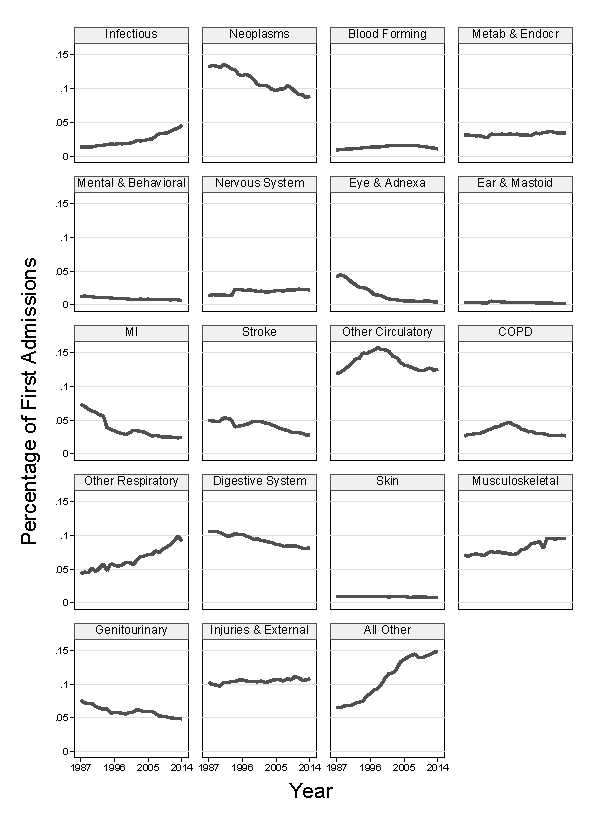
\includegraphics[scale=1.35]{Paper_3/Appendix_4.pdf}
		\caption*{\textbf{Figure Appendix 4:} 	Percentage of first hospital admission 
												at age 60+ by 19 cause specific groups 
												for yearly study population, 1987 to 
												2014. Cause specific categories constructed 
												from harmonized ICD-8 and ICD-10 codes 
												(Danish modification).}
	\label{ch4:app4}
	\end{figure}
	%--------------------%
	
	
%----------------------------------------------------------------%
%----------------------------------------------------------------%



%----------------------------------------------------------------%%----------------------------------------------------------------%

\chapter{Changes in the Demographic Profile of Hospital Patients}

%----------------------------------------------------------------%%----------------------------------------------------------------%

\vspace{0.5in}

\textbf{Paper:}
\textsc{\underline{Andreas H\"ohn}, Anna Oksuzyan, Rune Lindahl-Jacobsen, 
	    Roland Rau, and Kaare Christensen:} Preparing for the future: The 
	    changing demographic composition of hospital patients in Denmark 
	    between 2014 and 2050. \textbf{\textit{Submitted to a peer-reviewed journal}} 

%----------------------------------------------------------------%%----------------------------------------------------------------%

\newpage

\section{Abstract}
% BACKGROUND %
\textbf{Background:} Preparing the healthcare workforce for 
population aging is a public health challenge, especially as 
medical students tend to avoid the field of geriatrics. We 
describe the current demographic profile of hospital care use 
in Denmark, project changes up to 2050, and interpret this in 
the light of the attitudes of students in the healthcare 
workforce.\\ 
% METHODS %
\textbf{Methods:} The Danish population in 2014 (N=5.63 million) 
was followed up for inpatient and emergency admissions recorded 
in Danish hospitals in 2014 using population-based registers. We 
combined age and sex-specific patterns of hospital care use in 
2014 with official population estimates to forecast the profile 
of hospital days up to 2050 with respect to age and sex.\\ 
% RESULTS %
\textbf{Results:} The total number of hospital days per year is 
projected to increase by 47\% between 2014 and 2050, from 3.75 
to 5.51 million days. While small changes are projected among 
the population aged 0-69, the largest change is projected to 
occur among the population aged 70+. The 2014 levels were 0.77 and 
0.84 million days for men and women aged 70+, respectively. By 
2050, these levels are projected to have reached 1.76 and 1.63 
million days. Whereas the population aged 70+ accounted for 42.9\% 
of all days in 2014, their contribution is projected to increase 
to 61.4\% by 2050.\\
% CONCLUSION %
\textbf{Conclusion:} Specific attention should be given to the 
education of the future healthcare workforce, as negative 
stereotypes and prejudice towards older individuals are important 
factors discouraging medical students and student nurses from 
joining the field of geriatrics.\\


%----------------------------------------------------------------%%----------------------------------------------------------------%


\newpage


%%% Introduction %%%
\section{Introduction}

Decreasing mortality trends in high and middle income countries will 
rapidly increase the population share of older individuals within the 
next few decades.\citep{kontis2017future} Currently, in these countries, 
approximately one person in six is aged 65 or older. By 2050, it is projected 
that the number of people aged 65+ will have almost doubled within these 
countries, and that nearly one in three will be 65 or older.\citep{desa2017world}
As the prevalence of non-communicable diseases increases with age - including 
cancers,\citep{campisi2013aging} circulatory diseases,\citep{leening2014sex} 
and dementia\citep{rasmussen2018absolute} - population aging presents new 
challenges for healthcare systems, including hospital settings.\citep{beard2015towards,
pallin2014us} Preparing the medical workforce for the changing demographic 
profile of patients has been identified as one of these challenges.\citep{bodenheimer2009confronting} 
Efficient delivery of high-quality care requires an adequate supply of 
well-trained health workers to meet the needs of patients. Already, a number 
of countries have reported substantial shortfalls in skilled medical workers.\citep{darzi2016global}

A growing body of literature has reported that medical students and 
student nurses tend to have negative attitudes towards older individuals.\citep{samra2015medical,
kusumastuti2017contact,fisher2018pejorative} Working with older patients has 
often been described as a burden and as less satisfying than working with 
younger patients. Negative attitudes towards the elderly have been shown to 
be important predictors for the quality of care and treatment,\citep{wilson2018medical} 
and are one main reason why young medical professionals tend to avoid the 
field of geriatrics.\citep{hughes2008medical} Recent studies suggest that 
medical students are not aware of who their future patients will be.\citep{kusumastuti2017contact} 
This is problematic, as aging and retirement of the baby-boom generation will 
accelerate demographic changes, and are likely to leave holes in medical 
workforces.\citep{schofield2006demographic}

Forecasts of future levels of health expenditure are widely available. However, 
expenditure forecasts tend to be very sensitive to economic shocks and unforeseen 
changes in costs or new technologies.\citep{howdon2018health,breyer2010ageing} 
Less research effort has forecast changes in the levels and demographic profile 
of healthcare use, including hospital care. The profile of future hospital 
patients depends predominantly on changes in the demographic composition of the 
population, and is therefore easier to forecast than potential expenditures because 
a large proportion of future patients have already been born.\citep{dall2013aging} 
Previous forecasts of hospital care use have often focused on single causes of 
admission,\citep{vogl2016informing} or specific services only, such as long-term 
or palliative care.\citep{etkind2017many} Only a small body of literature has studied 
the effect of population aging on hospital care use patterns at the national level. 
While a small number of studies exist for Australia and the US,\citep{schofield2006demographic,
strunk2006effect} very little is known about changes in hospital care demand on 
country-level, and within the European healthcare context.

Here, we examine expected changes in the number of hospital days by age and sex 
in Denmark up to the year 2050 and interpret this in the light of the attitudes 
of students in the healthcare workforce.\\


%----------------------------------------------------------------%
%----------------------------------------------------------------%

\section{Methods and Materials}

\subsection{Linking Register Data}

This study utilizes routinely-collected register data, covering the entire 
Danish population. We used the unique personal identification number (CPR-Number), 
which is assigned to all individuals residing in Denmark, to link records from 
the National Patient Register (NPR) with data of the Central Population Registry 
(CPR). The CPR, established in 1968, contains demographic information, such as 
information on each resident's vital status, sex, and date of birth.\citep{pedersen2011} 
The NPR, a population-based register, covers administrative and medical information 
on all treatments provided in Danish hospitals since 1977.\citep{schmidt2015danish} 
The NPR data have high levels of completeness and reliability, making them 
a valuable data source for research.\citep{schmidt2015danish} \\

\subsection{Estimating Hospital Care Use Patterns from Linked Registers}

From the CPR, we identified 5,627,235 men and women alive and residing in Denmark 
on 1st January 2014, who were at risk of being admitted to hospital in 2014. These 
individuals were followed up for all inpatient and emergency admissions recorded 
in Danish hospitals between 1st January 2014 and 31st December 2014. We summed up 
the number of hospital days as well as the population at risk by age, and separately 
for men and women. We then divided the number of hospital days by the corresponding 
population at risk to obtain the average, annual number of hospital days per person 
by sex and age in 2014.

In contrast to inpatient admissions, information on outpatient treatments include 
the start date and the end date of the treatment period, but not the number of days 
an outpatient has received treatment in hospital. This makes it difficult to assign 
a number of hospital days per admission. In addition, obstetrics-related admissions 
have the potential to introduce a strong sex bias. We therefore excluded both, 
obstetric-related admissions and outpatient treatments, from our main analysis but 
included them in sensitivity analyses. \\

\subsection{Statistics Denmark's Population Projection}

We then identified the most recent population projection provided by Statistics 
Denmark, the Danish national statistical office,\citep{statden2018} and utilized 
its estimates of the Danish population covering the period 2018 to 2050. This is 
a so-called deterministic projection which makes forecasts on the basis of observed 
trends in fertility, mortality, and migration -- the only parameters that can affect 
the size and structure of a population -- up to the middle of the 21st century. The 
future trajectories of these parameters are assumed to be a reflection of current 
trends, and are based on levels which have been observed in Denmark within the last 
four years.\citep{statden2018} A detailed overview of the projection 
assumptions is given in \hyperref[ch5:tabS1]{Supplementary Table S1}.\\

\subsection{Forecasting the Hospital Care Use}

Lastly, we projected future numbers of hospital days by age and sex using a 
baseline forecast design.\citep{ganguly2016using} We kept the age- and sex-specific 
hospital care use patterns of 2014 constant throughout the entire study period and 
combined them with the population projection provided by Statistics Denmark. We 
multiplied the average, annual number of hospital days per person observed in 2014 
by the corresponding population in each year between 2018 and 2050, for single years 
of age and separately for men and women. As a result, we obtained the total annual 
number of hospital days by sex and single years of age, which we aggregated into four 
age groups, separately for men and women: 0-14, 15-49, 50-69 and 70+. The merging of 
registers was carried out with Stata (Version 14). Forecasts and Visualizations were 
produced with R (Version 3.5.1).\\


%----------------------------------------------------------------%
%----------------------------------------------------------------%


\section{Results}

\subsection{Hospital Care Use Patterns in 2014}

\hyperref[ch5:fig1]{Figure 1} shows the average number of hospital days per person in 2014 by age. 
The age trajectory of hospital care use is consistently J-shaped among men and 
women. Within the first year of life, the average number of hospital days per 
year is 0.7 days for men and 0.6 days for women. From age 1 onwards, the levels 
decline and reach a minimum of 0.1 days at age 9 among men and at age 8 among 
women. Thereafter, the levels plateau until age 30, at 0.1 to 0.2 days per year 
for men and women respectively. After age 30, the average number of hospital 
days per year starts to increase steadily with age, to 4.2 days and 3.3 days 
among men and women aged 90+, respectively. On average, women spend more days 
in hospital than men between ages 13 and 43. At age 44, the levels cross over 
and the annual number of days in hospital become lower among women than among 
men.\\

	%--------------------%
	\begin{figure}[H]
		\centering
		\includegraphics[scale=0.435]{Paper_4/MAIN_Figure_1.pdf}
		\caption*{\textbf{Figure 1:} Average number of days spent in hospital per person in 2014}
	\label{ch5:fig1}
	\end{figure}
	%--------------------%

\subsection{Changes in the Population Structure}

In 2014, the size of the Danish population was about 5.62 million. At that time, 
0.97 million individuals (17.3\%) were aged 0-14. The age group 15-49 consisted 
of 2.55 million individuals (45.4\%), while 1.43 million individuals (25.4\%) 
were aged 50-69. In 2014, 0.67 million Danes (11.9\%) were aged 70+, of whom 
0.29 million were men and 0.38 million were women.

Within the next decades, it is projected that the structure of the Danish population 
will change as the size of the population at older ages steadily increases. The 
projections up to 2050 are given in \hyperref[ch5:fig2]{Figure 2}. In 2050, it is forecast that the 
size of the Danish population will increase to 6.43 million. For the population 
younger than 70, only small changes in size are anticipated. By 2050, 1.05 million 
individuals (16.3\%) will be aged 0-14, 2.70 million individuals (42.0\%) will be 
aged 15-49, and 1.41 million individuals (21.9\%) will be of age 50-69. In contrast, 
major changes are expected in the older population. By 2050, it is projected that 
1.27 million Danes (19.8\%) will be aged 70 or older, of whom 0.59 million will 
be men and 0.68 million will be women. By this time, the size of the age group 70 
is forecast to have almost doubled in absolute terms.\\


	%-----------------------%
	\begin{figure}[H]
		\centering
		\includegraphics[scale=0.450]{Paper_4/MAIN_Figure_2.pdf}
		\caption*{	\textbf{Figure 2:} Projected changes in the structure of the Danish 
					population by sex between 2018 and 2050, based on publicly 
					available data provided by Statistics Denmark}
	\label{ch5:fig2}
	\end{figure}
	%-----------------------%


\subsection{Changes in Hospital Days}

In 2014, we observed 3.75 million hospital days in the Danish population. The 
population aged 0-14 accounted for 0.19 million days (5.0\%), the population aged 
15-49 0.66 million days (17.7\%), and the population aged 50-69 accounted for 1.29 
million days (34.5\%). In 2014, men and women aged 70+ contributed 0.77 and 0.85 
million hospital days respectively, together accounting for 42.9\% of all hospital 
days in that year.

We combined the age- and sex-specific hospital care use patterns of 2014 with 
Statistics Denmark's population projections to forecast the number of hospital 
days up to 2050. Results of the forecast are shown in \hyperref[ch5:fig3]{Figure 3}. 
The total number of hospital days per year is set to increase by 47\% within the observed 
period, reaching an overall level of 5.51 million days in 2050. The number of hospital 
days among the population younger than 70 is forecast to remain relatively stable 
during the projection period (Levels in 2050; 0-14: 0.21 million days (3.8\%) / 
15-49: 0.68 million days (12.7\%) / 50-69: 1.24 million days (22.5\%)). In contrast, 
the number of days accounted for by the population aged 70+ is projected to increase 
steadily and to more than double. By 2050, the population aged 70+ is forecast to 
account for 3.39 million days, or 61.4\% of all hospital days. Among the population 
aged 70+, men are expected to contribute 1.76 million days while women are expected 
to contribute 1.63 million days. This will correspond to 31.9\% and 29.5\%, respectively, 
of all hospital days in 2050.\\


	%-----------------------%
	\begin{figure}[H]
		\centering
		\includegraphics[scale=0.450]{Paper_4/MAIN_Figure_3.pdf}
		\caption*{	\textbf{Figure 3:} Projected annual number of hospital days until 2050}
	\label{ch5:fig3}
	\end{figure}
	%-----------------------%


\subsection{Sensitivity Analyses}

Our main findings do not include outpatient and obstetrics-related admissions. We 
examined the impact of these admissions on the age- and sex-specific patterns of 
health care use in 2014 and the projection of annual hospital days up to the year 
2050. We controlled separately for the impact of: (i) admissions due to childbearing 
and birth control, (ii) outpatient admissions, and (iii) a combination of both. 
Results of this robustness check (further discussed in \hyperref[ch5:textS1]{Supplementary Text S1}, and 
presented in \hyperref[ch5:figS1]{Supplementary Figure S1}, \hyperref[ch5:figS2]{Supplementary Figure S2}, 
and \hyperref[ch5:tabS2]{Supplementary Table S2} at the end of this paper) show 
similar trends and do not alter our conclusions. Irrespective of how we estimated 
the age- and sex-specific hospital care use in the baseline year 2014, the population 
aged 70+ remained the most important driver for the increasing amount of hospital 
days. In addition, men aged 70+ were always the fastest growing patient group treated 
in Danish hospitals in the period up to 2050. \\


%----------------------------------------------------------------%%----------------------------------------------------------------%


\section{Discussion}

In this study, we show the demographic profile of the demand for hospital 
care today and in the future. By keeping current age- and sex-specific patterns 
of hospital care use constant, we studied the changes attributable to population 
aging. Already today, the population aged 70+ accounts for half of all hospital 
days. We forecast that the absolute contribution of individuals aged 70+ to total 
hospital days will more than double and will account for nearly two thirds of all 
hospital days by 2050. By then, men aged 70+ are projected to be the largest 
patient group treated in Danish hospitals.\\
 
\subsection{Methodological Considerations}

We estimated the age- and sex-specific hospital care use patterns for the baseline 
year 2014 using routinely collected, individual-level register data. These data 
cover the total Danish population. Using register data eliminates recall biases, 
non-response and other problems regarding the under- or overstatement of healthcare 
use -- limitations which often affect studies based on self-reports.\citep{hunt2011women}

Forecasting is by its nature uncertain. This applies to two components of our 
projection: first, the structure of the Danish population and, second, patterns 
of hospital care use in the future. We used the most recent population projection 
of the Danish national statistical office. This projection is a deterministic 
projection and based on a continuation of current trends in fertility, mortality, 
and migration until the mid-21st century.\citep{denstat2018projection} Of all 
these parameters, future rates of migration are the most uncertain.\citep{de2010migration} 
Statistics Denmark assumes that in-migration will declines rapidly in the next 
few years, compared to the levels of 2015-2017, and will remain stable thereafter. 
We acknowledge that other projections do exist for Denmark, such as probabilistic 
projections by the United Nations.\citep{desa2017world} However, we decided to 
use the projections provided by Statistics  Denmark as they are the most recent 
and detailed for Denmark. 

Using a baseline forecast design, we froze the age- and sex-specific levels of hospital 
care use observed in 2014. Freezing rates assumes that age- and sex-specific patterns 
of hospital care use will remain constant in the future. Therefore, changes in the 
annual amounts of hospital days during the projection period are driven exclusively 
by changes in the demographic profile of the population. Keeping baseline levels 
constant during the projection period is a pragmatic approach in forecasting and 
has been applied to detailed projections of hospital care use\citep{vrhovec2016population} 
or fertility.\citep{bohk2018forecast} Especially when over-arching trends are 
difficult to predict, freezing rates has been shown to outperform statistically 
sophisticated techniques.\citep{bohk2018forecast} \\

\subsection{Health and Hospital Care Use in Aging Populations}

In line with previous findings, our study shows that hospital care use at late- 
and post-working ages is especially important for the total national hospital 
care demand. Previous research has shown that two opposite trends may have an 
impact on future hospital care use levels at these ages. On the one hand, the 
compression and postponement of morbidity may continue to reduce levels of hospital 
care use among the elderly.\citep{vaupel2010biodemography} Studies have shown 
that the incidences of leading causes of death, including stroke and MI, are 
consistently declining in low-mortality countries at all ages, including 
Denmark.\citep{schmidt201225} It has also been shown that cognitive functioning 
of the old and oldest-old has improved significantly within recent decades.\citep{christensen2013physical} 
Individuals of post-working age have been found to be increasingly happy 
and satisfied with their life considering the toll that aging generally 
takes on well-being, health and physical functioning.\citep{vestergaard2015physical}

On the other hand, it may be that the time spent with major chronic diseases 
does not shrink as life expectancy increases, and that frailty among the elderly 
even increases.\citep{clegg2013frailty} In addition, new medical technologies 
may contribute to increased treatment of this age group in hospitals, leading 
to higher levels of hospital care use in the future among the old and oldest 
old.\citep{oksuzyan2013changes} At the same time, these new technologies may 
enable a shift of treatments from inpatient to outpatient or primary healthcare 
settings. As both of these changes might have an impact at the same time, 
the general direction of population-level trends in hospital care use is difficult 
to predict. We therefore consider our findings to be neither overly optimistic -- 
nor pessimistic -- but to reflect a possible scenario.

Irrespective of long-term trends in age patterns and admission strategies, health 
behaviors impact population health and, as a consequence, future hospital care 
use. Studies show that smoking, hazardous drinking, obesity, lack of physical 
activity, and an unhealthy diet are associated with a higher risk of hospitalization 
at the individual level.\citep{hanlon2007analysis}  In Denmark, the general trend 
is towards healthier habits: smoking rates are decreasing, diet has improved, 
and physical inactivity has decreased.\citep{groth2014disparities} Future levels 
of hospital care use at the population level will be associated with the age pattern 
of diseases, trends in health behaviors within populations, as well as with the 
organizational structure and performance of healthcare systems. \\

\subsection{Implications of a Changing Patient Profile}

We forecast that the number of hospital days for individuals aged 70+ will almost 
double in the period up to 2050, as an increasing number of individuals reache 
older ages. The reason for this is rather simple: older individuals, on average, 
spend more days in hospital than younger individuals. Age is a major risk factor 
for non-communicable diseases and therefore directly linked with hospital care use 
levels.

Studies have shown that the prevalence of most leading causes of admission is 
likely to increase as the population ages, including circulatory diseases and 
cancers.\citep{christensen2009ageing} While more individuals survive to older 
ages, and better treatment of diseases reduces case fatality, the number of 
individuals at older ages with chronic conditions, complex diseases and multi-morbidity 
is increasing.\citep{christensen2009ageing} In the light of these findings, 
inadequacies in geriatric training for the medical workforce have to be addressed 
in order to meet the complex needs of older patients; this will involve changes 
in curricula, the role of senior staff, and the organizational structure of 
hospitals.\citep{samra2015medical} Addressing these deficiencies may encourage 
medical students and student nurses to join the field of geriatrics, and contribute 
to better treatment of the elderly.\citep{fisher2018pejorative} The education 
of healthcare workers is a long-term process and requires responsible and careful 
planning. Preparing healthcare services for changing needs requires an understanding 
of who the future patients will be. To meet future hospital care needs, reducing 
prejudice towards the elderly among medical students and student nurses has to be 
given special emphasis -- as soon as possible.\citep{fisher2018pejorative} Only 
sufficient numbers, and a well-balanced mix of specialists and sub-specialists, 
can ensure that the healthcare challenges of aging populations will be met in 
the coming decades.\citep{dall2013aging} \\

\subsection{Conclusion}

Already today, individuals of post-working age are the largest patient group 
in hospital settings. As populations age, the share of these age groups is 
projected to steadily increase. To ensure that hospitals meet the needs of 
future patients, a variety of responses are necessary. Reducing negative 
stereotypes and creating incentives to work with the elderly has to be one 
first step in order to ensure that future doctors and nurses are motivated 
and qualified to join the field of geriatrics. Taking into account the time 
frame to train medical staff, these issues should be addressed sooner rather 
than later. 


%----------------------------------------------------------------%%----------------------------------------------------------------%


\newpage


\section{Supplementary Material}
%%% Supplementary Text S1 %%%


\newpage


\begin{landscape}

%%% Supplementary Table S1 %%%
\begin{table}[H]
\scriptsize
\centering
\caption*{\textbf{Supplementary Table S1:} Overview on projection assumptions.}
\medskip
\begin{tabular}{llll}
\hline
\textbf{Process} & \textbf{Parameters}        & \textbf{(Sub-) Population} & \textbf{Value}                 
\\
\hline
                   &                         &                                                               &                         \\
\textbf{\textit{Mortality}}          & e(0) in 2059            & Men                                                           & 87.1 years              \\
                   & (Lee-Carter Method)     & Women                                                         & 89.5 years              \\
                   &                         &                                                               &                         \\
\textbf{\textit{Fertility}}          & Long-Term TFR           & Danish Origin - Danish Citizenship                            & 1.91                    \\
                   &                         & Danish Origin - foreign Citizenship                           & 1.91                    \\
                   &                         & Immigrants non-Western countries - Danish citizenship:        & 1.68                    \\
                   &                         & Immigrants non-Western countries - foreign citizenship:       & 1.97                    \\
                   &                         & Immigrants Western countries - Danish citizenship:            & 1.61                    \\
                   &                         & Immigrants Western countries - foreign citizenship:           & 1.77                    \\
                   &                         & Descendants from non-Western countries - Danish citizenship:  & 1.91                    \\
                   &                         & Descendants from non-Western countries - foreign citizenship: & 1.91                    \\
                   &                         & Descendants from Western countries - Danish citizenship:      & 1.75                    \\
                   &                         & Descendants from Western countries - foreign citizenship:     & 1.75                    \\
                   &                         &                                                               &                         \\
                   & Origin at birth         & Danish origin - Danish citizenship                            & 100.00                  \\
                   & (frequencies of change) & Danish origin - foreign citizenship                           & 100.00                  \\
                   &                         & Immigrants from non-Western countries - Danish citizenship    & 24.50                   \\
                   &                         & Immigrants from non-Western countries - foreign citizenship   & 21.80                   \\
                   &                         & Immigrants from Western countries - Danish citizenship        & 73.10                   \\
                   &                         & Immigrants from Western countries - foreign citizenship       & 36.40                   \\
                   &                         & Descendants from non-Western countries - Danish citizenship   & 100.00                  \\
                   &                         & Descendants from non-Western countries - foreign citizenship  & 41.40                   \\
                   &                         & Descendants from Western countries - Danish citizenship       & 100.00                  \\
                   &                         & Descendants from Western countries - foreign citizenship      & 66.30                   \\
                   &                         &                                                               &                         \\
\textbf{\textit{Out-Migration}}      & Number of out-migrants  & entire Danish population and all groups of origin             & N/A                     \\
                   &                         &                                                               & (not specified  \\
                   &                         &                                                               & as 2015--2017)   \\
                   &                         &                                                               &                         \\
\textbf{\textit{In-Migration}}       & Number of in-migrants   & Immigrants without Danish citizenship                         & 17,000                  \\
                   &                         & Western immigrants without Danish citizenship                 & 28,100                  \\
                   &                         & Reimmigration: Danish origin and all with Danish citizenship  & N/A                     \\
                   &                         &                                                               & (not  specified, \\
                   &                         &                                                               &  as 2015--2017)   \\ \hhline{====}
\end{tabular}
\label{ch5:tabS1}
\end{table}


\end{landscape}


%----------------------------------------------------------------%%----------------------------------------------------------------%


\newpage

\textbf{Supplementary Text S1:} Further Remarks on Sensitivity Analyses.\\

Our main findings do not consider outpatient admissions and obstetrics-related 
admissions \textbf{(Setting A)}. We investigated the impact of obstetrics-related 
admissions \textbf{(Setting B)}. We specified this category as O.00 -- O.99 and 
Z.30 -- Z.39 using the International Classification of Diseases (ICD), 10th Revision. In addition, 
we estimated the contribution of those outpatient treatments, which were provided 
within hospitals \textbf{(Setting C)}. Each outpatient treatment was approximated to contribute 
exactly one day. We used this approximation for outpatient admissions since the 
registers provide neither the exact number of days an outpatient has spent in the 
hospital, nor an overview of the provided services. Instead, the information in 
the registers on outpatient treatments covers the start and the end date of the 
treatment period for administrative purposes. We further studied the combined impact 
of outpatient treatments and obstetrics-related admissions \textbf{(Setting D)}.

\label{ch5:textS1}

While \hyperref[ch5:figS1]{Supplementary Figure S1} compares age- and sex-specific 
trajectories for the baseline year 2014 reflecting these four settings, 
\hyperref[ch5:figS2]{Supplementary Figure S2} compares the results of the 
corresponding projections. A summary of projection results for all four settings 
is presented in \hyperref[ch5:tabS2]{Supplementary Table S2}.\\


%----------------------------------------------------------------%%----------------------------------------------------------------%


%%% Supplementary Figure S1 %%%


\newpage


	%------------------%
	\begin{figure}[H]
		\centering
		\includegraphics[scale=0.45]{Paper_4/Supplementary_Figure_S1.pdf}
		\caption*{	\textbf{Supplementary Figure S1:} Average number of days spend 
					in hospital per person in 2014 by age and for different 
					admission types and causes.}
	\label{ch5:figS1}
	\end{figure}
	%--------------------%
	

%----------------------------------------------------------------%%----------------------------------------------------------------%


%%% Supplementary Figure S2 %%%


\newpage


	%------------------%
	\begin{figure}[H]
		\centering
		\includegraphics[scale=0.45]{Paper_4/Supplementary_Figure_S2.pdf}
		\caption*{	\textbf{Supplementary Figure S2:} Projected annual number of hospital 
					days up to the year 2050 for different admission types and causes.}
	\label{ch5:figS2}
	\end{figure}
	%--------------------%


%----------------------------------------------------------------%%----------------------------------------------------------------%


%%% Supplementary Table S2 %%%

\begin{landscape}



%%% PART I %%%
\begin{table}[htbp]
  \centering
  \caption*{	\textbf{Supplementary Table S2:} Comparing the impact of different 
  				specifications of hospital care use for 2014 (baseline year) and 
  				2050 (last year of the projection period).}
    \begin{tabular}{c|cc|cc|cc|cc}
    \toprule
    \multicolumn{9}{c}{\textbf{2014  - Men}} \\
    \midrule
    \textbf{Age} & \multicolumn{2}{c|}{\textbf{(A) Days in Hospital}} & \multicolumn{2}{c|}{\textbf{(B) Days in Hospital}} & \multicolumn{2}{c|}{\textbf{(C) Days in Hospital}} & \multicolumn{2}{c}{\textbf{(D) Days in Hospital}} \\
    \textbf{Group} & \textbf{N in Mio.} & \textbf{Share in \%} & \textbf{N in Mio.} & \textbf{Share in \%} & \textbf{N in Mio.} & \textbf{Share in \%} & \textbf{N in Mio.} & \textbf{Share in \%} \\
    \midrule
    0-14  & 0.10   & 2.66   & 0.10   & 2.51   & 0.33   &  4.14   &  0.33   &  4.03 \\
    15-49 & 0.31   & 8.31   & 0.31   & 7.84   & 0.95   &  11.88  &  0.95   & 11.48 \\
    50-69 & 0.72   & 19.30  & 0.72   & 18.19  & 1.30   &  16.33  &  1.30   & 15.73 \\
    70+   & 0.77   & 20.50  & 0.77   & 19.32  & 1.14   &  14.34  &  1.14   & 13.81 \\
    \midrule
    \textbf{All } & \textbf{1.90} & \textbf{50.77} & \textbf{1.90} & \textbf{47.86} & \textbf{3.72} & \textbf{46.69} & \textbf{3.72} & \textbf{45.05} \\
    \midrule
    \multicolumn{9}{c}{\textbf{2014  - Women}} \\
    \midrule
    \textbf{Age } & \multicolumn{2}{c|}{\textbf{(A) Days in Hospital}} & \multicolumn{2}{c|}{\textbf{(B) Days in Hospital}} & \multicolumn{2}{c|}{\textbf{(C) Days in Hospital}} & \multicolumn{2}{c}{\textbf{(D) Days in Hospital}} \\
    \textbf{Group} & \textbf{N in Mio.} & \textbf{Share in \%} & \textbf{N in Mio.} & \textbf{Share in \%} & \textbf{N in Mio.} & \textbf{Share in \%} & \textbf{N in Mio.} & \textbf{Share in \%} \\
    \midrule
    0-14  & 0.09  & 2.31  & 0.09  & 2.18  & 0.29  & 3.60  & 0.29  & 3.47 \\
    15-49 & 0.35  & 9.34  & 0.53  & 13.42 & 1.14  & 14.31 & 1.44  & 17.38 \\
    50-69 & 0.57  & 15.18 & 0.57  & 14.31 & 1.51  & 18.92 & 1.51  & 18.23 \\
    70+   & 0.84  & 22.41 & 0.88  & 22.23 & 1.31  & 16.47 & 1.31  & 15.87 \\
    \midrule
    \textbf{All } & \textbf{1.85} & \textbf{49.23} & \textbf{2.07} & \textbf{52.14} & \textbf{4.24} & \textbf{53.31} & \textbf{4.54} & \textbf{54.95} \\
    \midrule
    \textbf{Total} & \textbf{3.75} & \textbf{100} & \textbf{3.98} & \textbf{100} & \textbf{7.96} & \textbf{100} & \textbf{8.26} & \textbf{100} \\
    \bottomrule
    \bottomrule
    \end{tabular}%
\label{ch5:tabS2}
\end{table}%

  

%%% PART II %%%

\begin{table}[htbp]
  \centering
  \caption*{	\textbf{Supplementary Table S2 - Continued:} Comparing the impact of different 
  				specifications of hospital care use for 2014 (baseline year) and 
  				2050 (last year of the projection period).}
    \begin{tabular}{c|cc|cc|cc|cc}
    \toprule
    \multicolumn{9}{c}{\textbf{2050  - Men}} \\
    \midrule
    \textbf{Age} & \multicolumn{2}{c|}{\textbf{(A) Days in Hospital}} & \multicolumn{2}{c|}{\textbf{(B) Days in Hospital}} & \multicolumn{2}{c|}{\textbf{(C) Days in Hospital}} & \multicolumn{2}{c}{\textbf{(D) Days in Hospital}} \\
    \textbf{Group} & \textbf{N in Mio.} & \textbf{Share in \%} & \textbf{N in Mio.} & \textbf{Share in \%} & \textbf{N in Mio.} & \textbf{Share in \%} & \textbf{N in Mio.} & \textbf{Share in \%} \\
    \midrule
    0-14  & 0.11  & 2.03  & 0.11  & 1.96  & 0.37  & 3.45  & 0.37  & 3.35 \\
    15-49 & 0.32  & 5.83  & 0.32  & 5.62  & 0.99  & 9.38  & 0.99  & 9.11 \\
    50-69 & 0.69  & 12.54 & 0.69  & 12.08 & 1.25  & 11.83 & 1.25  & 11.46 \\
    70+   & 1.76  & 31.88 & 1.76  & 30.72 & 2.54  & 23.99 & 2.54  & 23.25 \\
    \midrule
    \textbf{All } & \textbf{2.88} & \textbf{52.28} & \textbf{2.88} & \textbf{50.38} & \textbf{5.14} & \textbf{48.65} & \textbf{5.15} & \textbf{47.17} \\
    \midrule
    \multicolumn{9}{c}{\textbf{2050  - Women}} \\
    \midrule
    \textbf{Age } & \multicolumn{2}{c|}{\textbf{(A) Days in Hospital}} & \multicolumn{2}{c|}{\textbf{(B) Days in Hospital}} & \multicolumn{2}{c|}{\textbf{(C) Days in Hospital}} & \multicolumn{2}{c}{\textbf{(D) Days in Hospital}} \\
    \textbf{Group} & \textbf{N in Mio.} & \textbf{Share in \%} & \textbf{N in Mio.} & \textbf{Share in \%} & \textbf{N in Mio.} & \textbf{Share in \%} & \textbf{N in Mio.} & \textbf{Share in \%} \\
    \midrule
    0-14  & 0.10   & 1.75  & 0.10   & 1.69  & 0.32  & 2.99  & 0.32  & 2.90 \\
    15-49 & 0.36   & 6.53  & 0.57   & 9.92  & 1.18  & 11.16 & 1.51  & 13.88 \\
    50-69 & 0.55   & 9.93  & 0.55   & 9.57  & 1.47  & 13.86 & 1.47  & 13.43 \\
    70+   & 1.63   & 29.51 & 1.63   & 28.44 & 2.47  & 23.35 & 2.47  & 22.62 \\
    \midrule
    \textbf{All } & \textbf{2.63} & \textbf{47.72} & \textbf{2.84} & \textbf{49.62} & \textbf{5.43} & \textbf{51.35} & \textbf{5.76} & \textbf{52.83} \\
    \midrule
    \textbf{Total} & \textbf{5.51} & \textbf{100} & \textbf{5.72} & \textbf{100} & \textbf{10.57} & \textbf{100} & \textbf{10.91} & \textbf{100} \\
    \bottomrule
    \bottomrule
    \end{tabular}%
\end{table}%

\end{landscape}


%-------------------------------------%


% REFERENCES %
\footnotesize
\bibliographystyle{vancouver}	
\bibliography{BIB_ALL_ABR_NONUM_2019-11-05}
	
%-------------------------------------%

\backmatter

%-------------------------------------%

\end{document}
